\newpage
\phantomsection
%\chapter{Computational adaptive optics for phase unstable OCT systems}
\chapter[Computational aberration correction in phase-unstable OCT: SHARP]{Computational aberration correction in phase unstable OCT: SHARP}\label{chap:SHARP}

There are several techniques for computational aberration correction in OCT as presented in previous chapter, all relying on a phase stability requirement to successfully operate the complex OCT signal. The core proposal of this work is described in detail in this chapter, a technique called SHARP to carry out CAO in tomograms having two dimensional phase noise, capable of correcting $x$-$y$-separable aberrations in tomograms affected by phase-jitter noise, which typically appears as 2D phase noise. The foundation of the method are presented in Section~\ref{sec:SHARP}, starting with the description of a tool for the assessment of phase stability and the validation of Nyquist sampling, following with an illustration of attempts to 2D phase stabilization, to show the impossibility to succeed with current fully numerical correction and to explain the motivation behind the operation of SHARP, and by the end of the section, the steps of the method are described and explained in detail. Then, results from a proof of concept experiment are presented in Section~\ref{sec:Test}, to evaluate the performance of SHARP in experimental datasets and determine if its purposed is well accomplished. Finally, complementary steps for SHARP are explained in Section~\ref{sec:Extensions}, oriented to solve specific issues not covered by the general proposal, in order to increase its applicability and improve results in particular situations.

\section{SHARP: A CAO technique for OCT}\label{sec:SHARP}

\subsection{Phase stability and sampling assessment}

Although phase stability of a system can be roughly estimated by imaging an ideal reflective surface and computing the phase difference between consecutive A-lines, this is not useful in practical situations to estimate phase stability in tomograms of real samples unless there is a reference reflective surface. Here, a tool for qualitative assessing phase stability and sampling in any complex tomogram is presented, based on the sample signal information itself and its acquisition process, as devised in a previous work~\cite{Cuartas-Velez2017_Formacion}.

Consider the lateral Fourier transform of the acquired signal $\hat{S}(x,y;z_d)$ for the low-NA regime in Eq.~\eqref{eq:CAO}, which can be written as
\begin{equation}
    \hat{S}(q_x, q_y; z_d) = H(q_x, q_y, z_d) \hat{\eta}(q_x, q_y, z_d),
\end{equation}
where the phase term in Eq.~\eqref{eq:CAO} is included in the frequency filter $H$, that can be described as $H(q_x,q_y, z_d)=\Omega(q_x, q_y, z_d)e^{i\varphi(q_x, q_y, z_d)}$, being $\Omega(q_x, q_y, z_d)$ its amplitude and $\varphi(q_x, q_y; z_d)$ its phase. Although the phase of $H$ varies with depth, its amplitude can be approximated to be constant over depth, and it follows a Gaussian distribution in the case that the input collimated beam in the scan lens of the system is also Gaussian-distributed (as it is in standard systems), this can be noted in the amplitude term $e^{-q^2\alpha^2/4k^2}$ of the forward model in Eq.~\eqref{eq:f^2}. Now, the power spectrum $\xi = |\hat{S}|^2$ of the signal is
\begin{align}
    \xi(q_x, q_y, z_d) &= |H(q_x, q_y, z_d) \hat{\eta}( q_x, q_y, z_d)|^2 \nonumber\\
    &= |\Omega(q_x, q_y)e^{i\varphi(q_x, q_y, z_d)} \hat{\eta}(q_x, q_y, z_d)|^2 \nonumber\\
    &= |\Omega(q_x, q_y)|^2 |\hat{\eta}(q_x, q_y, z_d)|^2.
\end{align}

The power spectrum of the sample $|\hat{\eta}(q_x, q_y, z_d)|^2$ is in general unknown but it is known to be a random distribution, given the random scattering property that characterizes tissue. Therefore, the expected value over depth of $|\hat{\eta}(q_x, q_y, z_d)|^2$ will yield a flat, nearly constant power spectrum $\gamma$, thus the mean power spectrum (MPS) $\bar{\xi}$ of the acquired discrete signal, averaged over $N_z$ depths planes, is given by
\begin{align}
    \bar{\xi}(q_m, q_n) &= \frac{1}{N_z}\sum_{l=1}^{N_z}\left|\text{FT}_{m,n}\{S(m,n,l)\}\right|^2\nonumber\\
%    &\approx \frac{1}{N_z}\sum_{l=1}^{N_z}|\Omega(q_m, q_n)|^2 |\hat{\eta}(q_m, q_n, l)|^2 \nonumber\\
    &\approx \frac{1}{N_z}|\Omega(q_m, q_n)|^2 \sum_{l=1}^{N_z} |\hat{\eta}(q_m, q_n, l)|^2 \nonumber\\
    &\approx \frac{1}{N_z}\gamma|\Omega(q_m, q_n)|^2,
\end{align}
where $(q_m,q_n)$ are discrete indexes for $(q_x,q_y)$, and because $\Omega$ follows a Gaussian distribution, then \textbf{the MPS $\bar{\xi}$ is also expected to follow a Gaussian distribution}. However, the latter is true assuming that the are not phase or amplitude disturbances on the signal $S(x,y,z)$, implying that the MPS is indeed a potential tool to evaluate phase stability.

Phase noise affecting local phase stability manifests as high frequency disturbances in the OCT signal, thus the Fourier transform of the signal will be distorted, presenting more high-frequency content than expected and therefore the MPS will no longer follow a Gaussian distribution. In other words, \textbf{the MPS of a tomogram with local phase stability follows a Gaussian distribution} whereas the MPS of a tomogram with local phase instabilities follows a non-Gaussian distribution, approaching a flat distribution. This ``rule of thumb'' on the analysis of the MPS is useful to determine whether a certain tomogram has enough phase stability for a successful operation of any CAC technique.

In the presence of global or long-range phase noise, the MPS will be only slightly affected given that such phase noise manifests as low-frequency content that is less significant than the low-frequency content of the Gaussian function. Such observation is important given that numerical phase stabilization method described in Section~\ref{sec:phaseStabilization} yields only local phase stability and not global, yet the analysis on the MPS is valid for such case.

To visualize the previous explanations, Figure~\ref{fig:MPSExample} shows the MPS of the simulated tomogram used for Fig.~\ref{fig:CAO} that is intrinsically phase stable as shown in Fig.~\ref{fig:MPSExample}(a), and also the MPS after inducing phase noise consisting in phase offsets randomly distributed across A-lines to illustrate the MPS of a phase-unstable tomogram, which has a nearly flat distribution as observed in Fig.~\ref{fig:MPSExample}(b). Although the phase-stable MPS in Fig.~\ref{fig:MPSExample}(a) approximates to a Gaussian function, residual non-constant contributions of the sample frequency content appears when not sufficient depth planes $N_z$ are available (in this case $N_z = 256$). This, however, do not prevent the analysis on the MPS in practical terms because the Gaussian distribution dominates.

\begin{figure}[htb!]
	\centering
	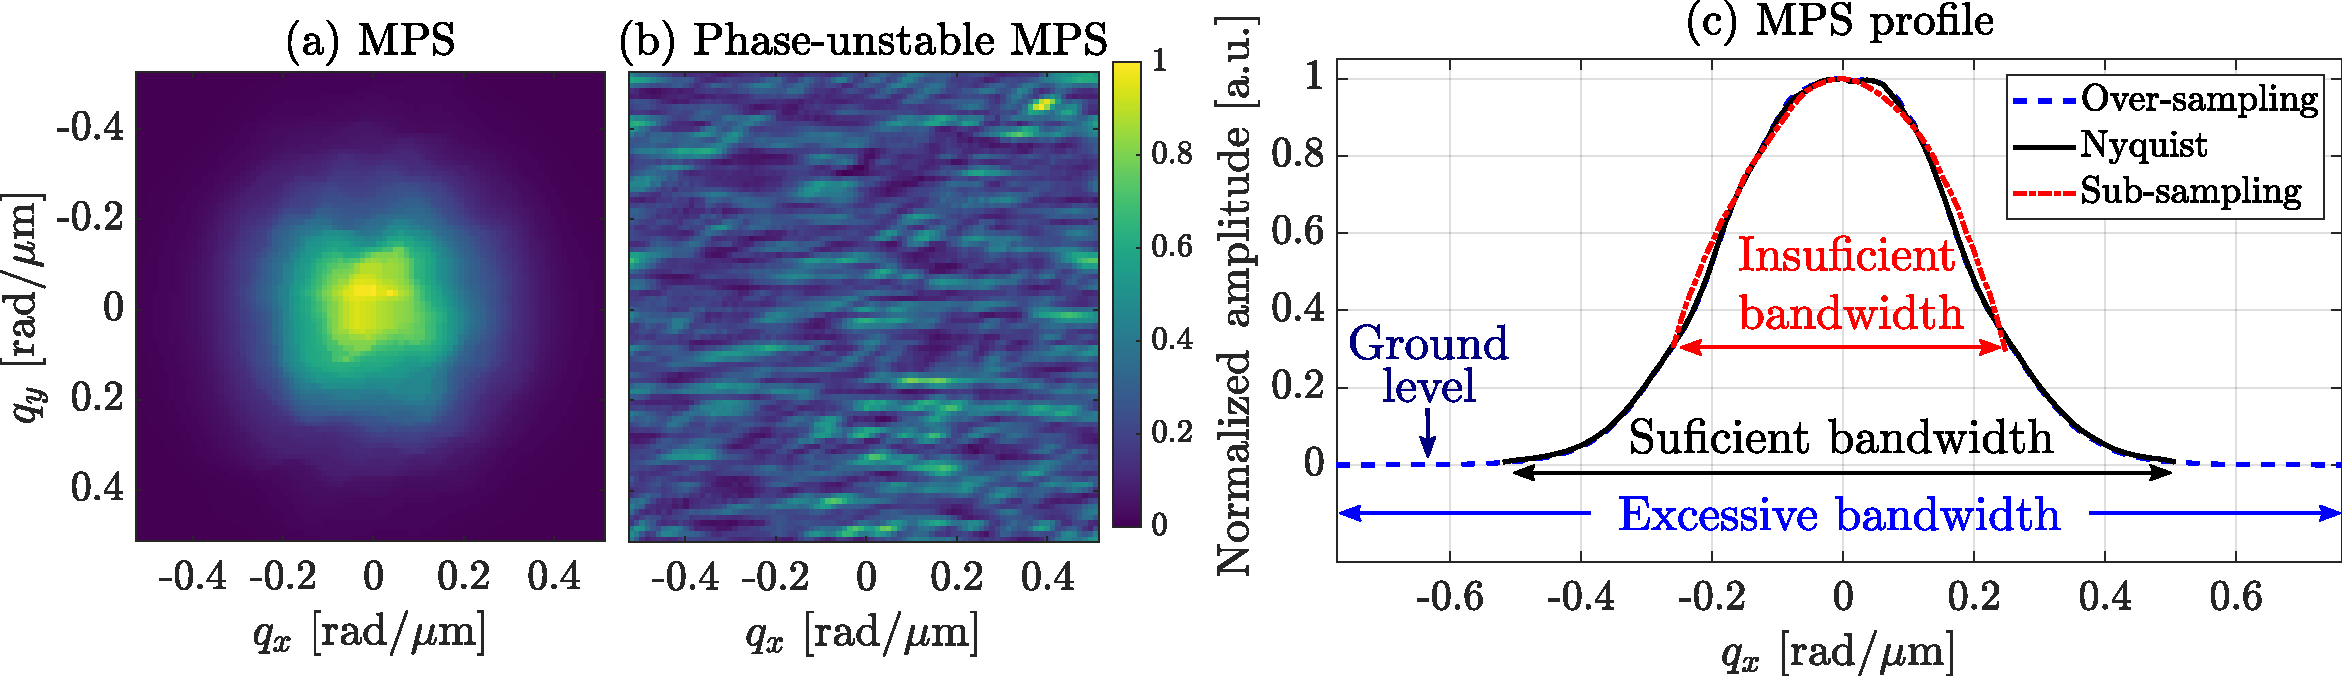
\includegraphics[width=\textwidth]{Figures/SHARP/PhaseStabilization/MPSExample.pdf}
	\caption[Illustration of the mean power spectrum with a simulated OCT tomogram.]{Illustration of the mean power spectrum with a simulated OCT tomogram. (a) MPS of raw tomogram, (b) MPS of tomogram with induced phase noise, and (c) 1D profile of the MPS averaging along $q_y$, for the tomogram using different samplings.}
	\label{fig:MPSExample}
\end{figure}

On the other hand, given the importance of a correct sampling for the operation of CAC techniques, it is worth to discuss the impact of sampling on the MPS, depicted in Fig.~\ref{fig:MPSExample}(c). Gaussian shape of the MPS is related to the fact that the optical system acts as a low-pass filter with cutoff frequency $f_c$ defined by the spatial resolution, thus the bandwidth of the Gaussian function is determined by the spatial resolution. The MPS will be truncated depending on the sampling, therefore changing sampling will not change the width of the Gaussian MPS, it will just truncate the Gaussian distribution depending on the sampling frequency. A \textit{correct/incorrect} sampling of the tomogram will result in a \textit{sufficient/insufficient} frequency bandwidth of the Gaussian-shaped MPS. as it is explained below.

It is known that Nyquist frequency $f_N = 2f_{\text{max}}$ provides the sufficient frequency bandwidth to correctly sample a signal with a known maximum frequency $f_{\text{max}}$, which in this case is determined by the lateral resolution $f_{\text{max}} = 1 / \delta x$, thus $f_N=2/\delta x$. In the case of having a correctly sampled tomogram (i.e. sampling less than $\delta x$/2), the frequency content will extend at least or beyond $f_c$, which means that the frequency bandwidth is \textit{sufficient} to capture the Gaussian shape of the MPS, as occurs in blue and black curves in Fig.~\ref{fig:MPSExample}(c) corresponding to the MPS of over-sampled and Nyquist-sampled tomograms, respectively. In the opposite case of having an incorrectly sampled tomogram (sampling greater than $\delta x$/2) the frequency content will be truncated before $f_c$, thus the frequency bandwidth is \textit{insufficient} to capture the Gaussian shape of the MPS, as occurs with red curve in Fig.~\ref{fig:MPSExample}(c) that corresponds to the MPS of a sub-sampled tomogram, which do not reaches the ground level, contrary to the other two curves. Therefore, \textbf{a tomogram with correct sampling will exhibit a MPS that captures the entire effective bandwidth of its Gaussian shape}, this means that the high frequency content reaches the ground level, which is essentially zero but in practical terms will be the noise floor level.

The two previous analysis on the MPS are therefore useful tools to determine that certain tomogram satisfies the two main requirements for successful operation of CAC techniques: phase stability and fulfillment of Nyquist theorem~\cite{Ruiz-Lopera2020_Computational}. The MPS can be used to analyze the phase stability provided by the fully numerical phase stabilization method described in Section~\ref{sec:phaseStabilization} that is of particular interest here. To do so, the simulated phase-unstable dataset used to exemplify the MPS in Fig.~\ref{fig:MPSExample} was corrected using the phase differences of A-lines along $x$ to compute the phase-jumps correction. Figure~\ref{fig:PhaseStable1D-enface} shows \textit{en face} phase images of the original tomogram, that is intrinsically phase stable [Fig.~\ref{fig:PhaseStable1D-enface}(a)], of the tomogram with induced random phase-jumps, that is 2D phase-unstable [Fig.~\ref{fig:PhaseStable1D-enface}(b)] and after correcting phase-jumps along $x$ axis, resulting in phase stability only along this axis [Fig.~\ref{fig:PhaseStable1D-enface}(c)]. The original tomogram is 2D phase-stable as indicated by the 2D Gaussian shape of its MPS shown in Fig.~\ref{fig:PhaseStable1D-enface}(d), whereas phase-corrupted tomogram exhibits a nearly flat MPS in the two axes as shown in Fig.~\ref{fig:PhaseStable1D-enface}(e). Instead, the phase-corrected tomogram exhibits 1D phase stability, and this yields a MPS with Gaussian shape only along one axis, in this case $x$ axis, whereas the orthogonal dimension remains phase unstable and thus with a flat MPS as depicted in Fig.~\ref{fig:PhaseStable1D-enface}(f). To verify that indeed 1D phase stability is achieved after correction, the 1D profile of the MPS in $x$ axis can be computed by averaging along $q_y$ axis, and this is shown in Fig.~\ref{fig:PhaseStable1D-enface}(e), where the 1D MPS of the original and phase-corrected tomograms approximate to a similar Gaussian shape, but corrupted tomogram has a constant MPS. Equivalent results are obtained if phase correction is computed using phase differences of A-lines along $y$ axis instead of $x$ axis, except that now the only phase-stable axis will be $y$.

\begin{figure}[htb!]
	\centering
	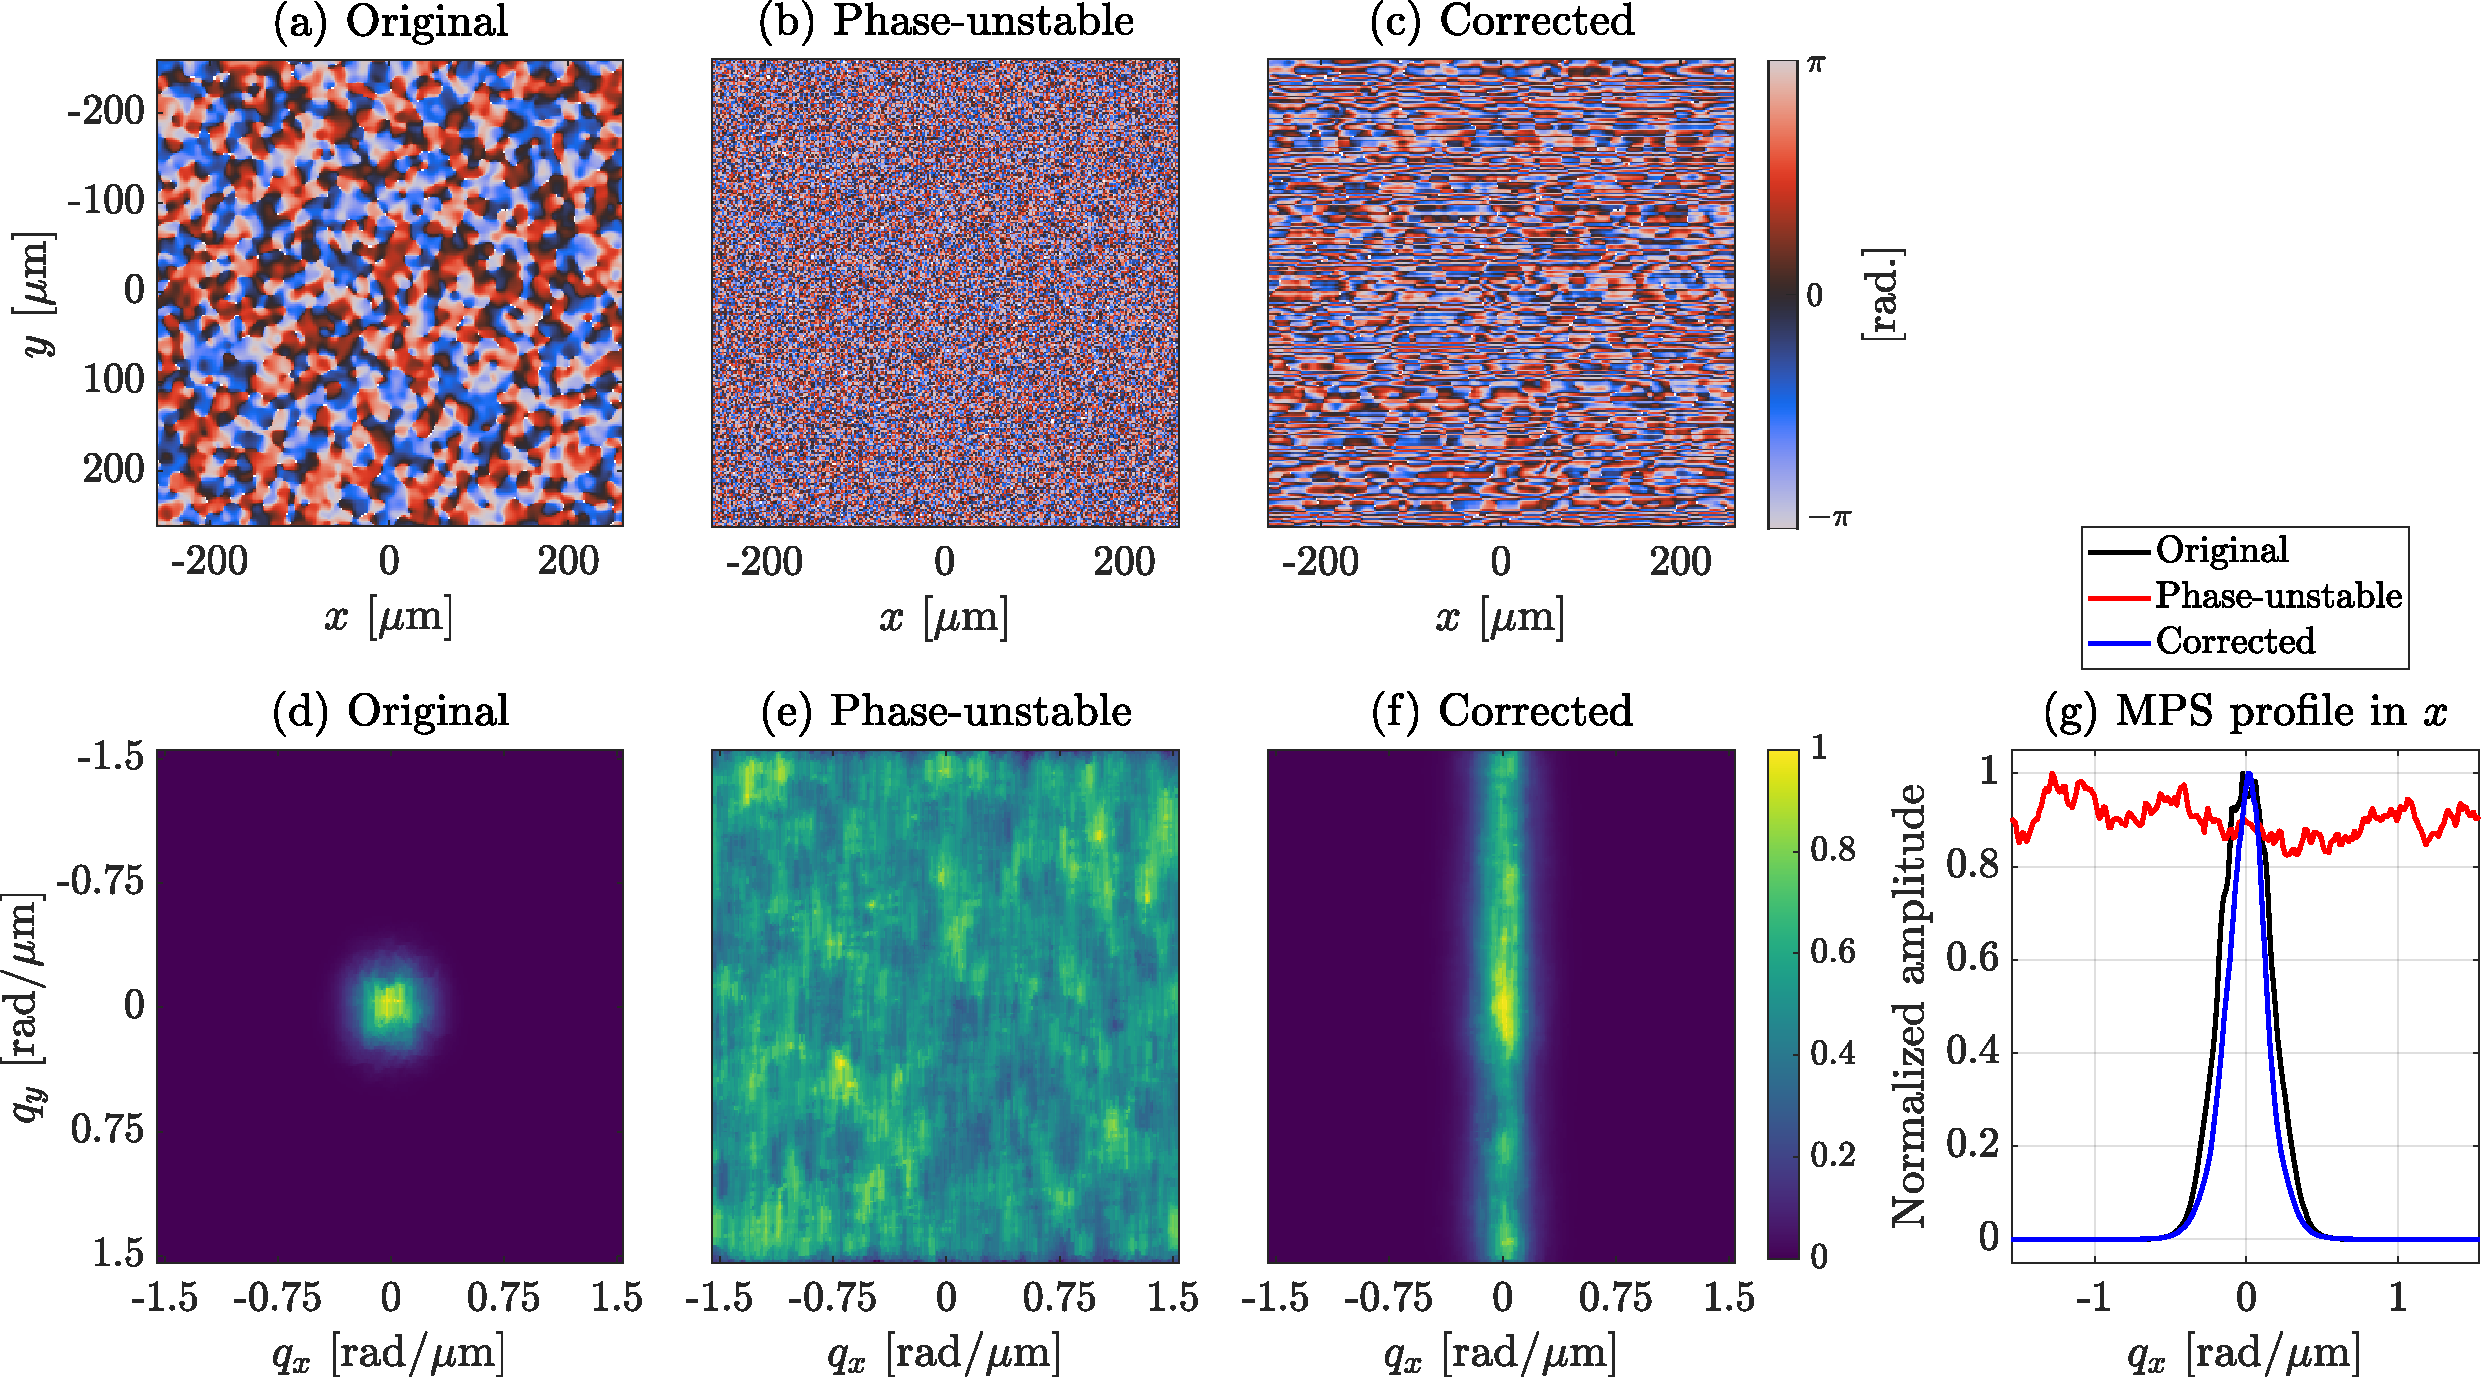
\includegraphics[width=\textwidth]{Figures/SHARP/PhaseStabilization/PhaseStabiliaztion1D-enface.pdf}
	\caption[Illustration of the mean power spectrum after phase correction with a simulated OCT tomogram.]{Illustration of the mean power spectrum after phase correction with a simulated OCT tomogram. \textit{En face} phase images: (a) original, (b) phase-unstable with random phase-jumps and (c) phase corrected along $x$. (d)-(f) MPS images of (a)-(c), respectively. (g) 1D profile of the MPS by averaing (d)-(f) along $q_y$.}
	\label{fig:PhaseStable1D-enface} 
23

\end{figure}
\FloatBarrier

\subsection{Attempts to 2D phase stabilization}

The presence of 2D phase noise requires a 2D correction but the fully numerical phase stabilization described previously is insufficient since its operation is intrinsically 1D. Two particular expansions of the phase stabilization method could be devised in order to achieve 2D phase stability, however, it is shown here that such attempts do not succeed as well as any stabilization based on traditional 1D phase correction.

First intuitive attempt to 2D phase stabilization is to perform two successive 1D phase corrections along the two scan axes. However, it has been found that the second correction would destroy the first correction hence, at the end, phase stability is achieved only along the axis that was corrected last. Results from this proposal were obtained using the phase-unstable simulated dataset used for Fig.~\ref{fig:PhaseStable1D-enface} and are illustrated in Figure~\ref{fig:PhaseStable2D} showing cross-sectional images of the plane $z$-$x$ (B-scan) and the orthogonal plane $z$-$y$. The phase-unstable tomogram was corrected along $x$ axis and resulting cross-sectional views are shown in Figs.~\ref{fig:PhaseStable2D}(a) and (b), exhibiting phase stability in the plane $z$-$x$ but not in the plane $z$-$y$. After the first correction, phase was corrected along $y$ axis expecting to obtain 2D phase stability but instead phase is corrupted again in the plane $z$-$x$ and only the plane $z$-$y$ is stable, as shown in Figs.~\ref{fig:PhaseStable2D}(c) and (d) which demonstrate that two consecutive 1D phase stabilization is not suitable to correct 2D phase noise. Because B-scan phase images are representative of a single plane, it is useful to analyze the MPS in order to know the general behavior of the entire tomogram. The $x$ and $y$ profiles of the MPS of the tomogram corrected only in $x$ and the one corrected in both axes are shown in Figs.~\ref{fig:PhaseStable2D} (g) and (h). Note that the MPS of the tomogram corrected only along $x$ is phase stable in this axis [black curve in Fig.~\ref{fig:PhaseStable2D}(g)] but it is phase unstable in $y$ axis [black curve in Fig.~\ref{fig:PhaseStable2D}(h)], contrary to the MPS of the tomogram corrected consecutively along the two axes [red curves in Figs.~\ref{fig:PhaseStable2D}(g) and (h)].

% \begin{figure}[htb!]
% 	\centering
% 	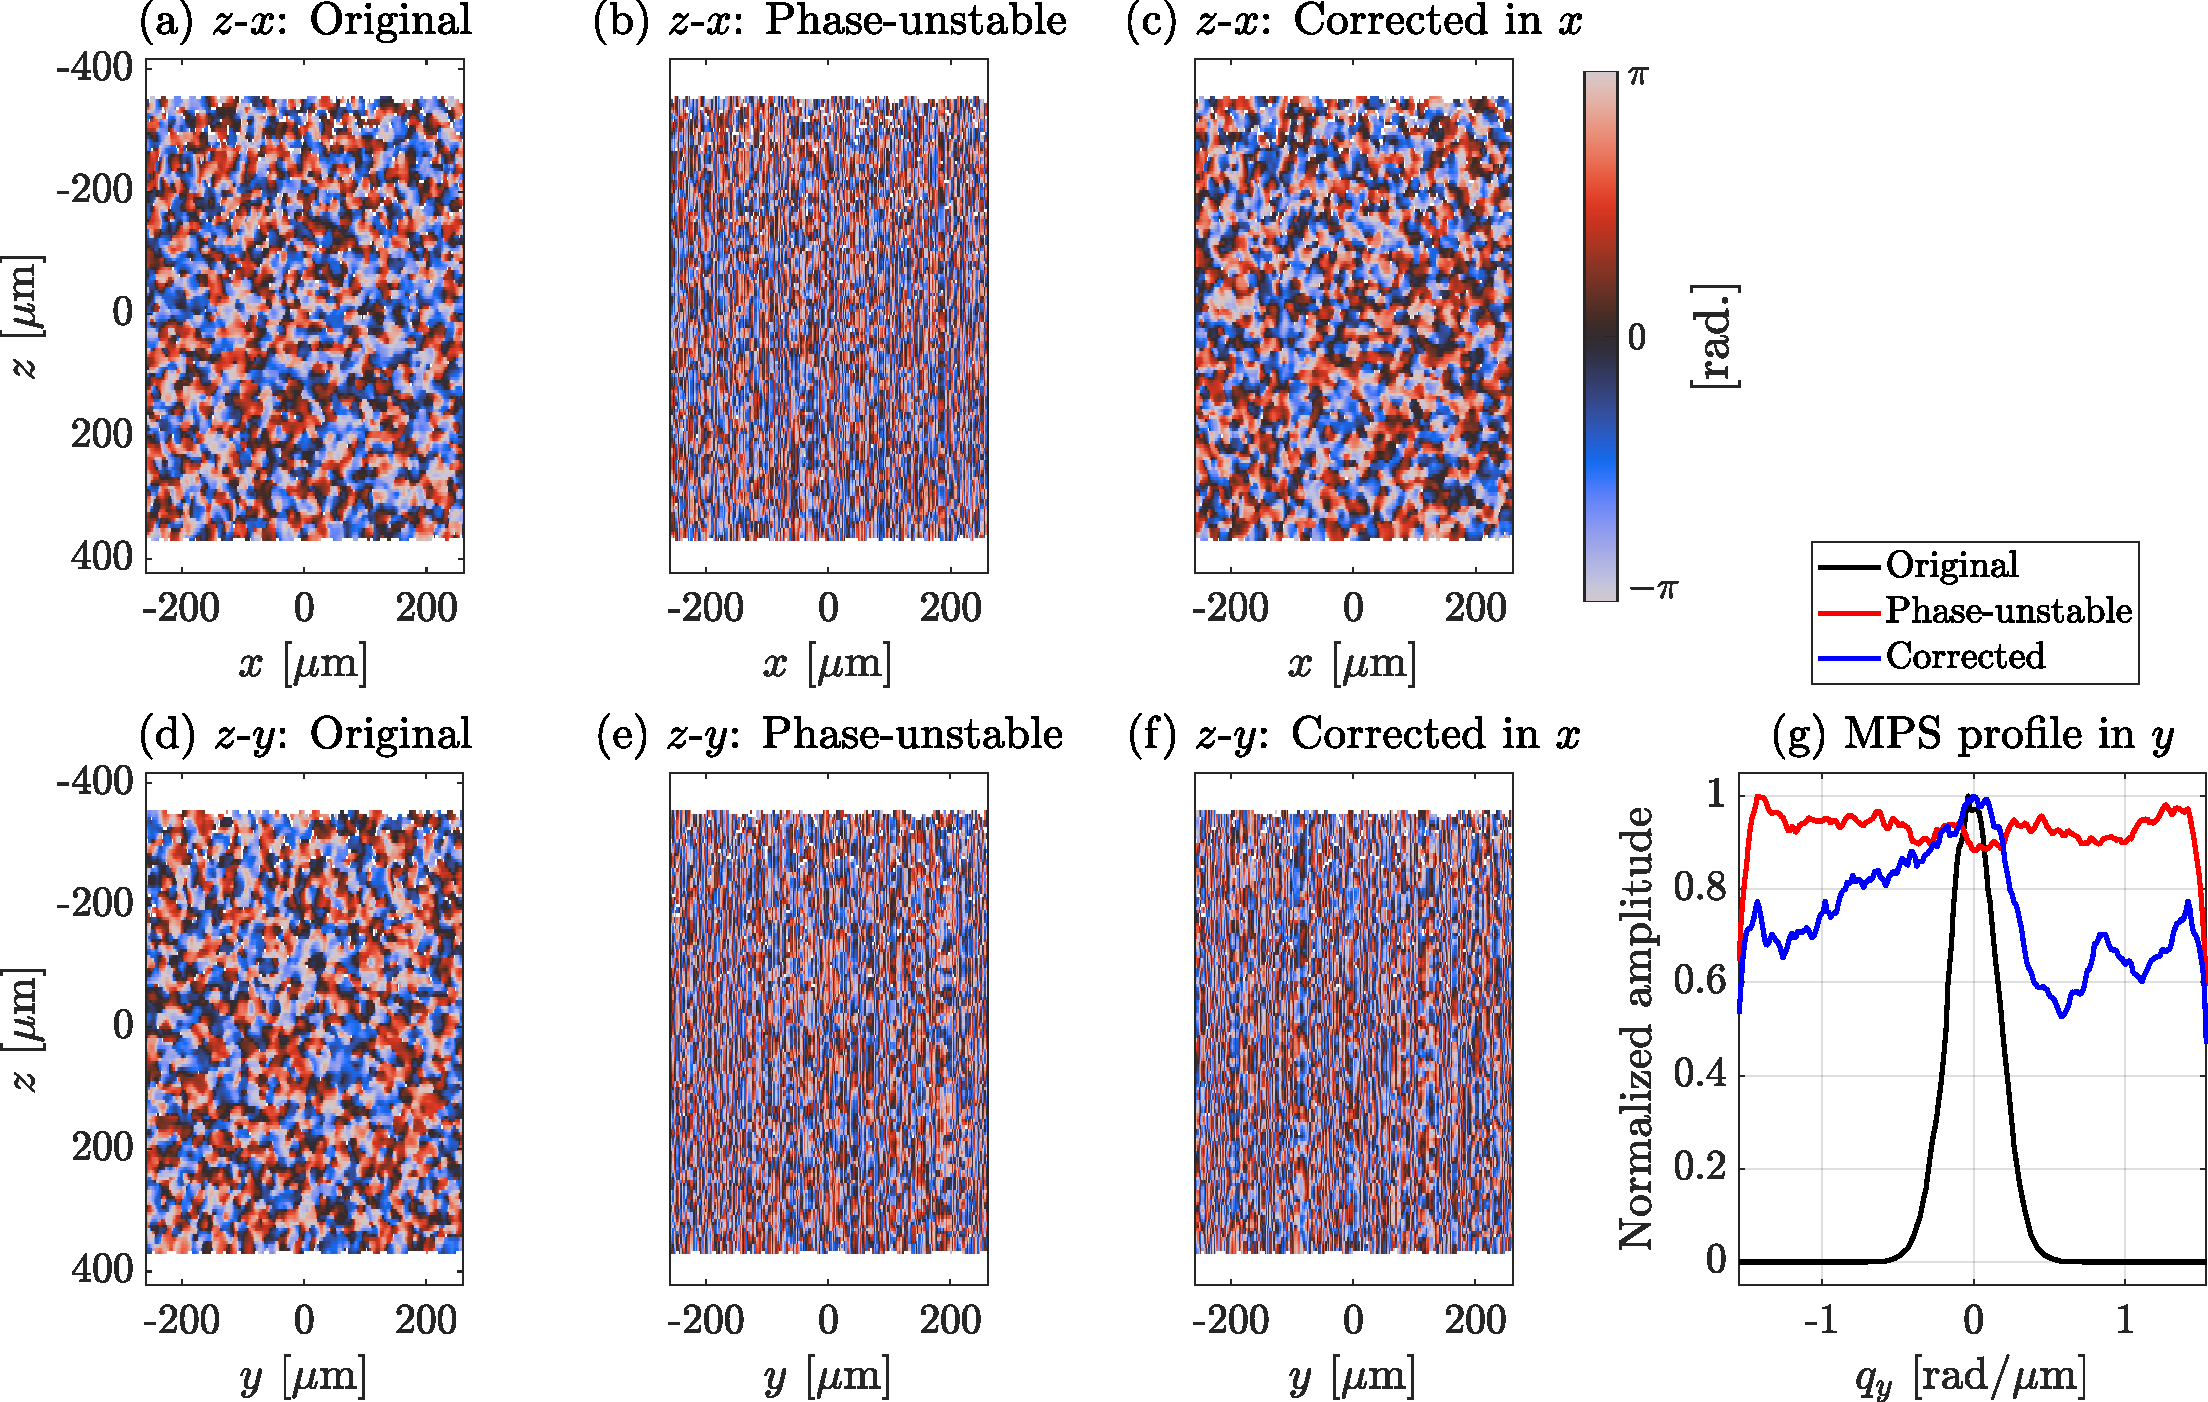
\includegraphics[width=\textwidth]{Figures/SHARP/PhaseStabilization/PhaseStabiliaztion1D.pdf}
% 	\caption[]{}
% 	\label{fig:PhaseStable1D}
% \end{figure}

\begin{figure}[htb!]
	\centering
	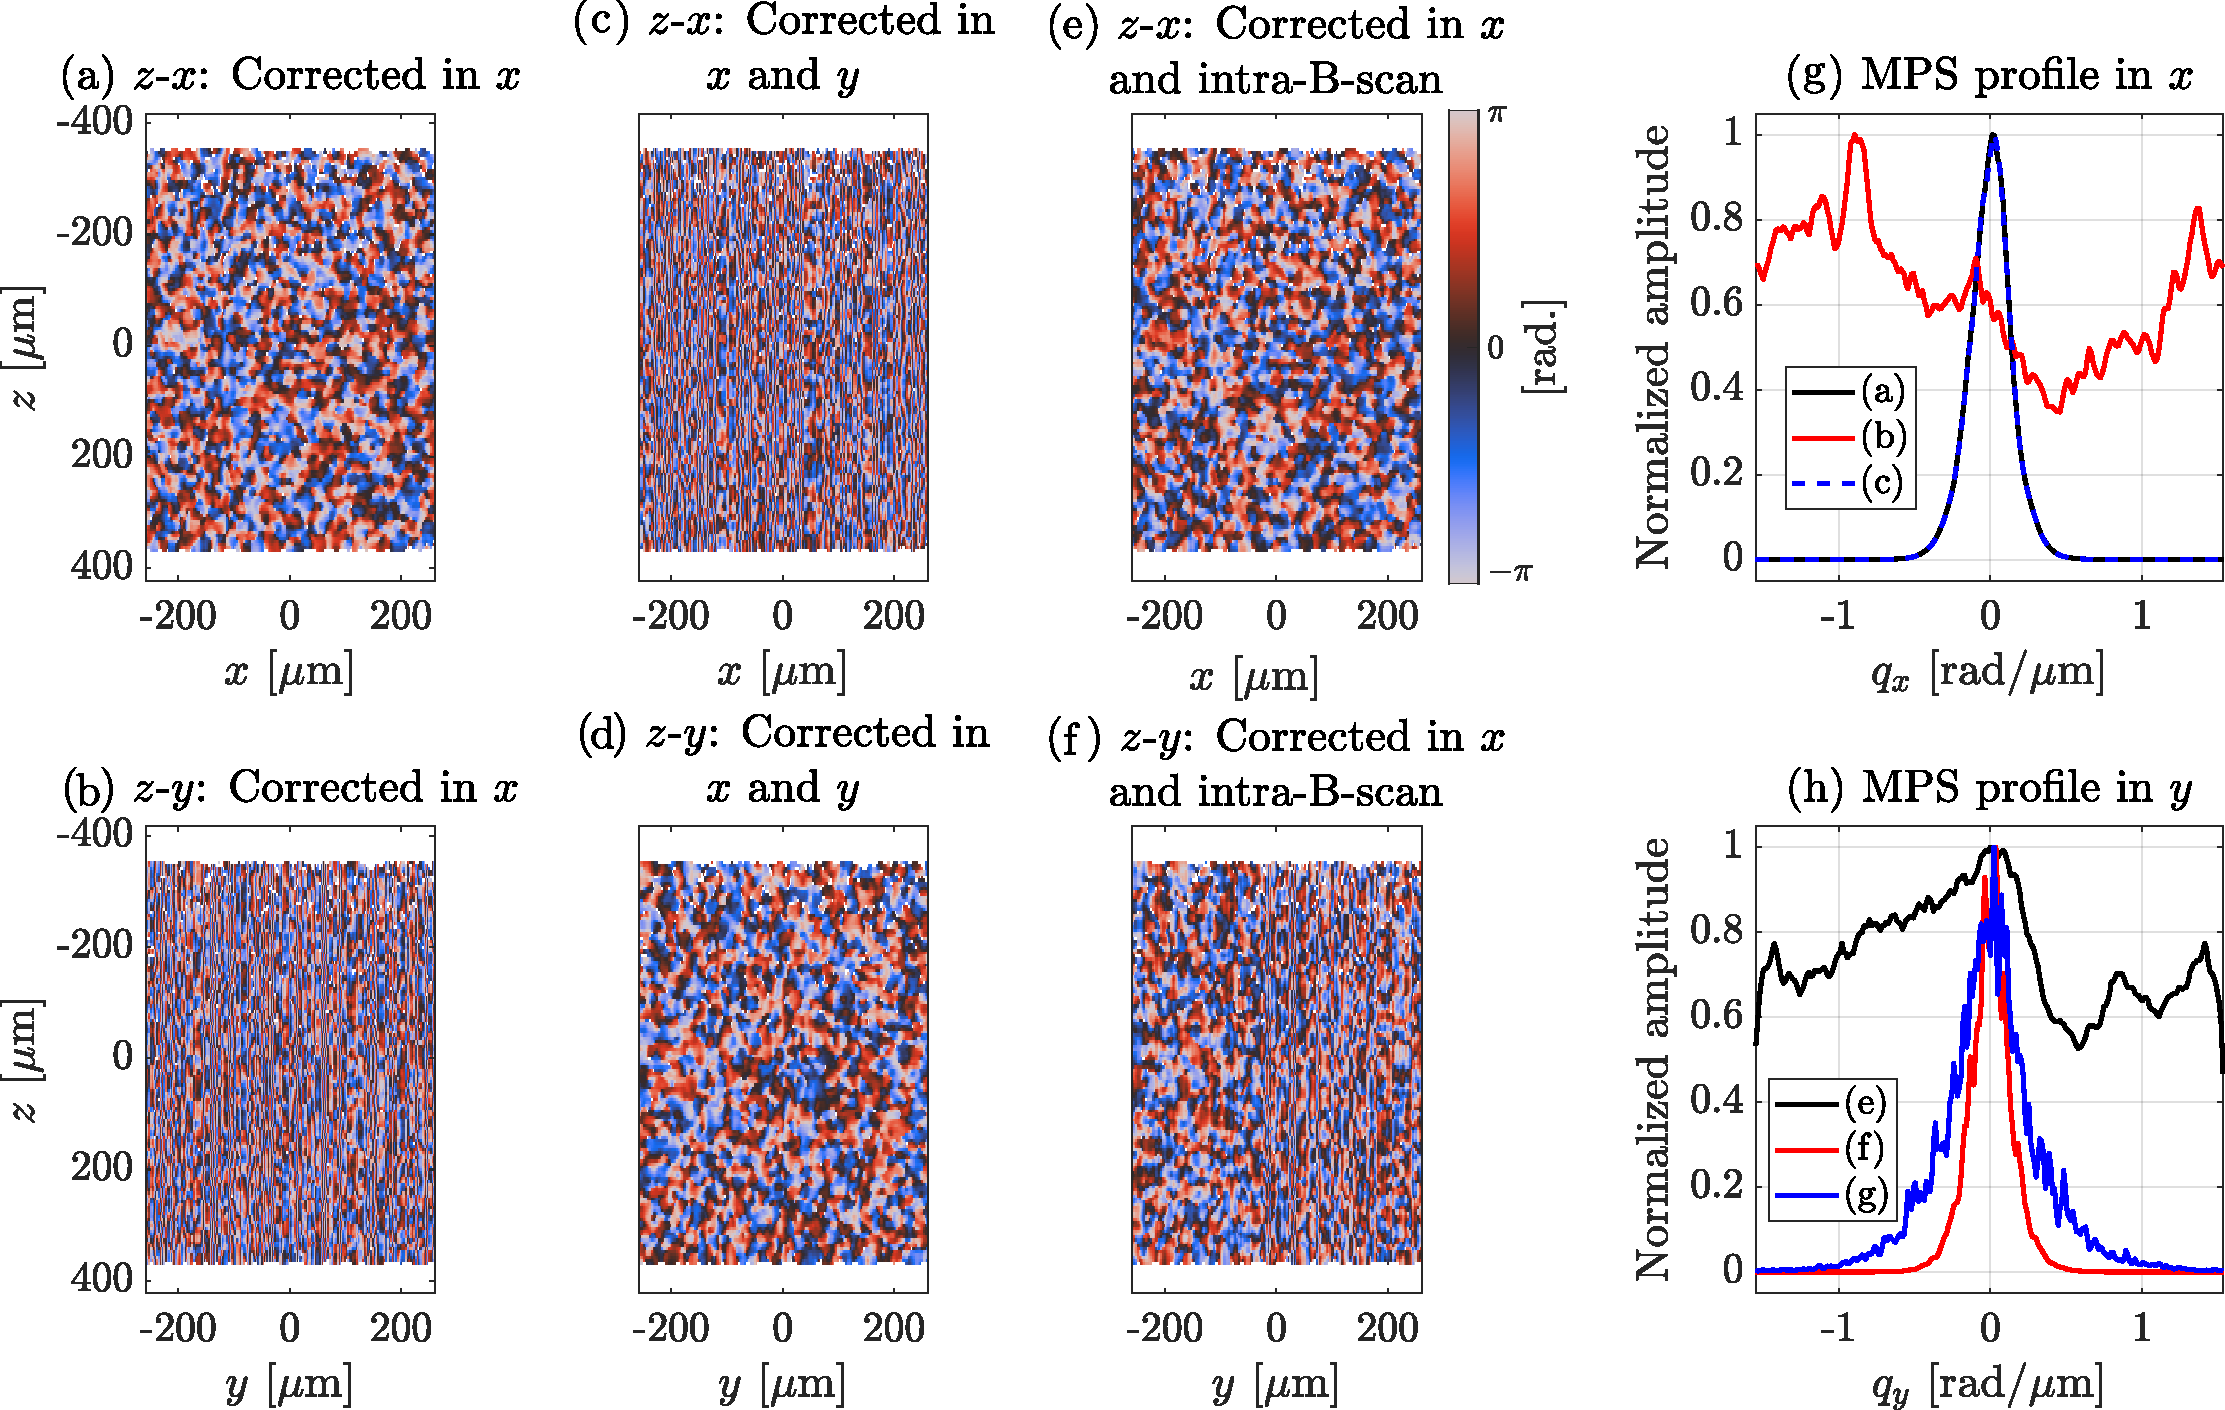
\includegraphics[width=\textwidth]{Figures/SHARP/PhaseStabilization/PhaseStabiliaztion2D.pdf}
	\caption[Illustration of attempts to 2D phase stabilization with a phase-unstable simulated dataset.]{Illustration of attempts to 2D phase stabilization with a phase-unstable simulated dataset. Cross-sectional views of: (a)-(b) tomogram corrected along $x$ axis, (c)-(d) tomogram corrected along $x$ axis and then along $y$ axis, (e)-(f), tomogram corrected along $x$ axis and then inter-B-scan. (a),(c),(e) are views of $z$-$x$ planes and (b),(d),(f) of $z$-$y$ planes. 1D Profile of the MPS: (g) in $x$ axis and (h) in $y$ axis.}
	\label{fig:PhaseStable2D}
\end{figure}

A second attempt to 2D phase stabilization is to correct the phase along one axis, and then to correct only for residual global phase noise between consecutive planes in the orthogonal axis, and this way the first correction will not be destroyed as in previous proposal. For instance, if phase is corrected along $x$, resulting in the corrected tomogram $\tilde{S}(m,n,l)$, then the second correction would be computed using the phase difference between A-lines along $y$ axis, that are then averaged along $x$ axis to obtain a global correction for each B-scan, instead of obtaining an individual correction for each A-line. The global corrections $\Delta_n$ between B-scans (or simply inter-B-scan) are calculated as
\begin{align}
    \delta(n) &= \arg\left\{\sum_{l=1}^{N_z} \sum_{m=1}^{N_x} S(m,n,l) S^*(m,n-1,l)\right\} \nonumber\\
    \Delta(n) &= \sum_{\hat{n} = 1}^n\delta(\hat{n}),
\end{align}
and applied as
\begin{equation}
    \tilde{\tilde{S}}(m,n,l) = \tilde{S}(m,n,l) e^{-i\Delta(n)},
\end{equation}
where $N_x$ is the number of A-lines in $x$ axis and $N_z$ is the number of depth samples, also note that $\Delta(n)$ is a function of B-scan index $n$ only. The purpose of the inter-B-scan correction is to correct for errors along the second axis without destroying phase stability along the first axis since it is a global correction for each B-scan. The latter is well-accomplished as noted in the B-scan phase image in Fig.~\ref{fig:PhaseStable2D}(e) that was corrected in $x$ and then inter-B-scan, but the inter-B-scan correction seems insufficient to correct for phase noise along $y$ axis as noted in Fig.~\ref{fig:PhaseStable2D}(f), which appears to be phase stable only in the left portion of the image, but not towards the right region, suggesting that a global correction is not sufficient. This is also observed in the MPS profiles; MPS in $x$ axis [blue curve in Fig.~\ref{fig:PhaseStable2D}(g)] is almost identical to that corrected only along $x$, but MPS in $y$ axis [blue curve in Fig.~\ref{fig:PhaseStable2D}(h)] exhibits residual high frequency content that suggests significant residual phase noise.

The impossibility to correct for 2D phase noise using traditional 1D phase stabilization may arise because small local errors, insignificant for local phase stability, are induced in the process and they propagate along the orthogonal direction as a consequence of the cumulative sum used to compute the global corrections, resulting in long-range errors that randomly disrupt the phase along this axis and frustrate any attempt to obtain 2D phase stability using 1D corrections.

\subsection{Description of the method}

In order to enable the operation of CAC techniques in tomograms with 2D phase noise like those acquired with SS-OCT systems presenting phase-jitter, it is possible to develop a scheme that leverage from 1D phase stability instead of aiming to succeed in 2D phase stabilization which is so far not possible with traditional phase correction. Here a novel technique is proposed for computational correction of aberrations in OCT tomograms with 2D phase noise, that leverages from the fact that 1D short-range phase stability is sufficient to perform the deconvolution operation in which CAC techniques are grounded, from this arises the name of the technique \textbf{SH}ort \textbf{A}line-\textbf{R}ange \textbf{P}hase-stability adaptive-optics (SHARP)~\cite{Ruiz-Lopera2020_Computational}.

SHARP integrates sequential 1D numerical phase noise and aberration correction steps and can operate in tomograms with phase noise arising from phase-jitter, galvanometer scanners and sub-resolution sample axial bulk motion, as long as Nyquist sampling is fulfilled. SHARP is suitable for OCT systems with no special hardware phase reference signals nor specialized configurations that ensure phase stability along any scan axis like those used often in the context of CAO, in particular, it is compatible with standard SS-OCT systems, affected by 2D phase noise.

The procedure consists in two sequential steps linked by an intermediate step as follows. First, phase noise is corrected along one axis $u$ (being $u$ either $x$ or $y$) followed by a 1D aberration compensation in that axis. Secondly, phase noise correction in $u$ is rolled-back by applying the inverse correction to the 1D \emph{corrected} tomogram. Then, phase noise is corrected along the other axis $v$, orthogonal to $u$, followed by a 1D aberration compensation in $v$, yielding a 2D computationally aberration-corrected volume. The intermediate rollback (RB) step is a key step to remove the long-range phase errors introduced in the first correction that would frustrate the second phase correction, and thus it enables the second CAC step.

A flowchart summarizing the procedure is shown in Figure~\ref{fig:SHARPFlowDiag}. $S_{m,n,l}$ is the input aberrated, phase-unstable tomogram, $\mathbb{C}_u\left\{\cdot\right\}$ represents the phase stabilization procedure applied along a generic axis $u$  and $\mathbb{C}_u^{-1}\left\{\cdot\right\}$ is its inverse meaning that the inverse phase correction is applied to cancel out the initial correction, $\mathbb{A}_u\left\{\cdot\right\}$ represents the aberration correction procedure applied along a generic axis $u$, and $\tilde{S}^{\text{1D}}_{m,n,l}$ and $\tilde{S}_{m,n,l}$ are the output, aberration-corrected tomograms, being $\tilde{S}_{m,n,l}$ the two-dimensional corrected tomogram that is the general interest, and $\tilde{S}^{\text{1D}}_{m,n,l}$ the one-dimensional aberration-corrected tomogram that is the aim in certain applications where 2D aberration correction is not possible for specific reasons subject to the application, for instance in catheter-based imaging. An optional, additional step is to rollback the second phase noise correction, thus recovering the original phase unstable tomogram but with aberrations already corrected, and this could be useful to combine SHARP with other phase-dependent techniques that would be carried out after application of SHARP.

\begin{figure}[htb!]
	\centering
	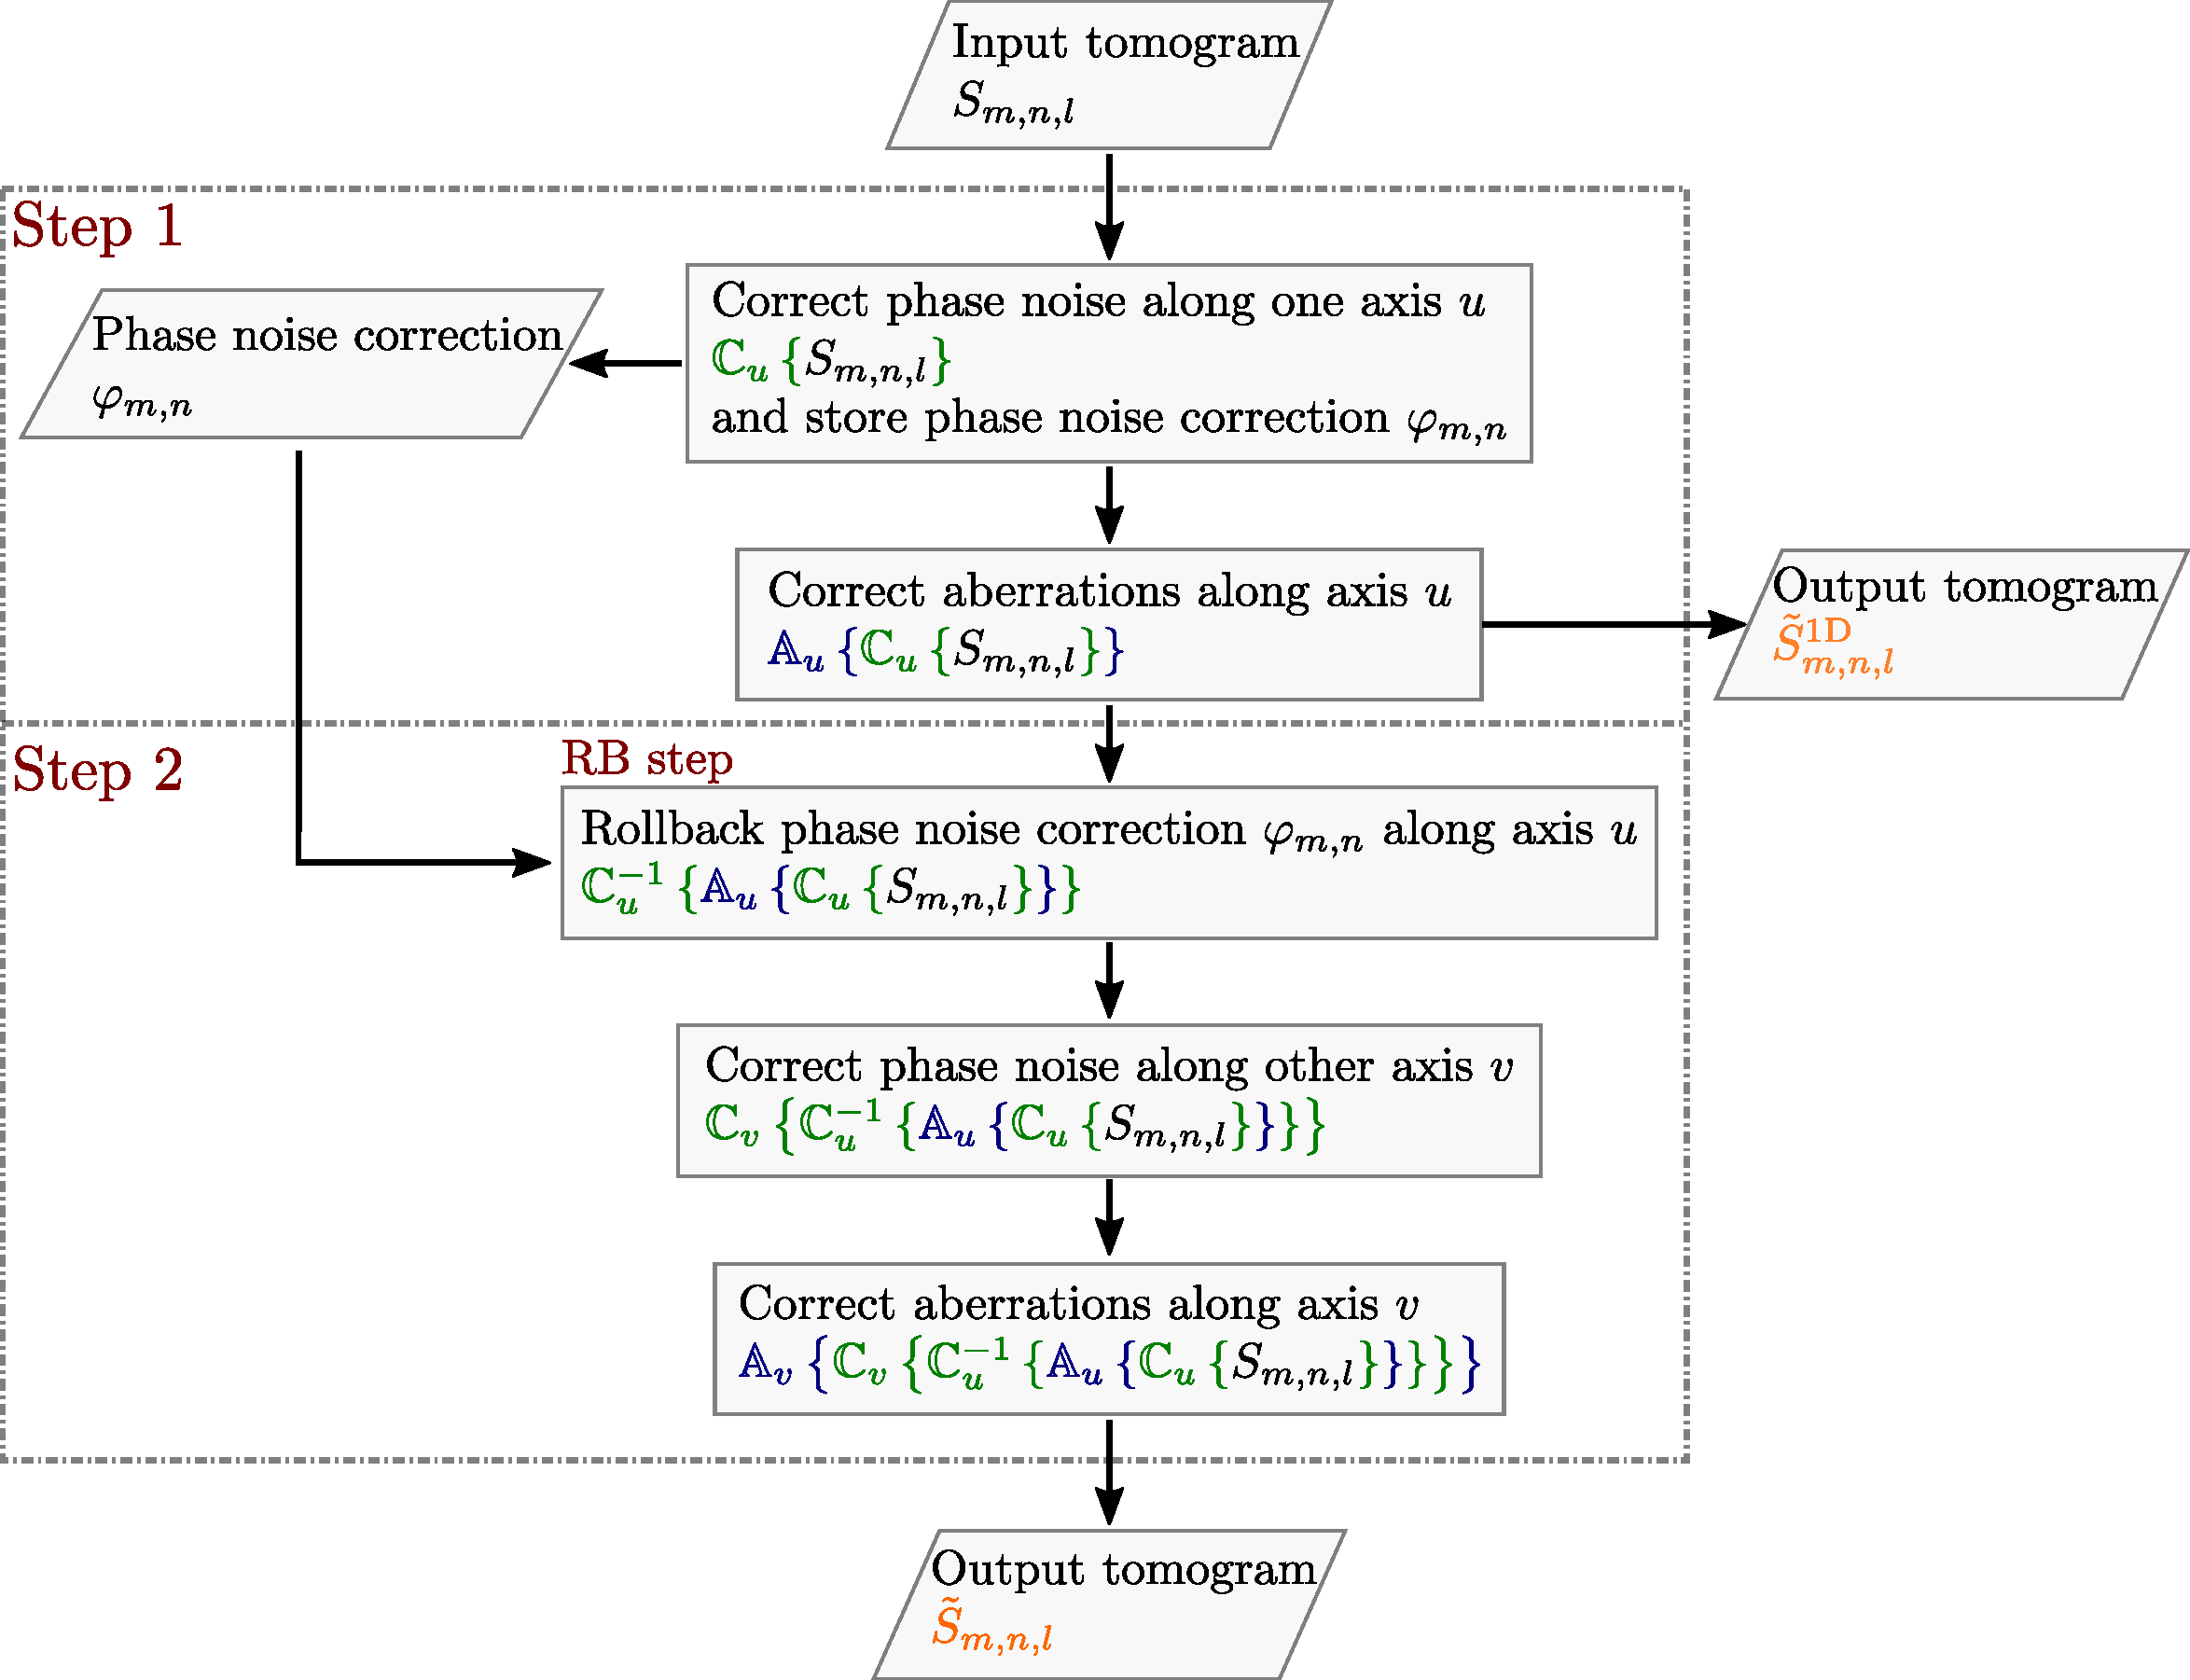
\includegraphics[width=\textwidth]{Figures/SHARP/BlockDiagram.pdf}
	\caption[Flowchart of the SHARP procedure.]{Flowchart of the SHARP procedure.}
	\label{fig:SHARPFlowDiag}
\end{figure}
\FloatBarrier

\subsubsection{Phase noise correction}

For the phase noise correction steps, a modification of the fully numerical method described in Section~\ref{sec:phaseStabilization} is used in order to address phase-jitter noise in addition to phase-offsets already covered by the method. The phase differences between consecutive A-lines along the axis of interest, for instance $x$ axis, are computed similarly to Eq.~\eqref{eq:PhaseDiff} as
\begin{equation}
    \delta(m,n,l) = \arg\left\{S(m,n,l)S^*(m-1,n,l)\right\}
\end{equation}
except that instead of summing along depth as in Eq.~\eqref{eq:PhaseDiff}, a linear fit of the form $\hat{\delta}(m,n,l) = b_0(m,n) + b_1(m,n)l$ is performed on $\delta(m,n,l)$ in order to estimate the phase offsets $b_0(m,n)$, arising from all potential sources such as galvanometer scanners or axial motion, as well as slopes $b_1(m,n)$ arising from phase-jitter noise. In other words, phase noise of each A-line is characterized by a phase-ramp noise with offset $b_0(m,n)$ and slope $b_1(m,n)$, with both parameters changing randomly across A-lines. Finally, phase correction operator $\mathbb{C}_x\left\{\cdot\right\}$ is applied to correct for phase-ramp noise as
\begin{align}\label{eq:phaseDiffJitterCor}
   \mathbb{C}_x\left\{S(m,n,l)\right\} &= e^{i\hat{\Delta}(m,n,l)} S(m,n,l) \nonumber\\ \text{where} \ \ \ \hat{\Delta}(m,n,l) &= \exp\left\{\sum_{\hat{m} = 1}^m \hat{\delta}(\hat{m},n,l)\right\}.
\end{align}

The exact same produce is applied to correct along $y$ axis, making $y$ as the variable of interest ($n$ in discrete notation). Logarithmic intensities of the conjugate products $10\log_{10}\left\{|S_{m,n,l}S^*_{m-1,n,l}|^2\right\}$ are used as weights to perform a weighted-linear fit. Furthermore, a mask is applied to ignore those pixels with logarithmic intensity below a threshold value, typically set to the noise floor level which in general can be approximated to be constant over the tomogram.

Given that the phase of a complex quantity is defined in the range [$-\pi,\ \pi$], phase wrapping may appear in Eq.~\ref{eq:phaseDiffJitterCor} if the phase-ramp exceeds these boundaries. It was already explained that phase wrapping is not an issue for phase-offsets correction (Section~\ref{sec:phaseStabilization}), but for the case of phase-slopes, wrapping can influence the linear fit, resulting in an erroneous correction. Therefore, phase unwrapping prior to the linear fit would be desirable to provide a more confident correction, however, it is challenging to perform an adequate phase unwrapping of the OCT signal given the presence of noise and speckle, and in practical terms it has been found that phase wrapping is not as critical as anticipated in this particular case. To clarify this, first consider that SS-OCT systems are equipped with a sampling clock to produce a trigger signal, typically using a fiber Bragg grating, so that the magnitude of phase-jitter is generally below one sampling cycle, equivalent to slopes below $2\pi$, being this the limit for phase wrapping, and timing jitter greater than two or three sampling cycles is seldom observed, in a standard system in normal conditions.

Furthermore, although imaging range of SS-OCT systems is typically of $\sim$6~mm, the effective axial range covered by tissue is in general equal or less than half the imaging range due to light absorption in the tissue. This means that the range where the phase-ramp is fitted is actually less than half the imaging range, reducing the susceptibility to phase-wrapping because only a portion of the ramp is used and not its entire extension. For instance, a timing jitter of two sample clocks results in a phase-ramp with effective range $4\pi$ in the full axial range but only with effective range $2\pi$ if the half axial range is used. Finally, before performing the linear fit, global phase offsets computed by averaging $\delta(m,n,l)$ along depth are subtracted to $\delta(m,n,l)$ in order to avoid the phase-ramp starting at a value where it could wrap.

Further experimental validation of SHARP will demonstrate that in practical terms these considerations and strategies are sufficient for the linear fit in the phase correction procedure despite the lack of phase unwrapping.

\subsubsection{Aberration correction: Phase filter}

For the aberration correction step, the idea behind SHARP is to perform two 1D independent corrections instead of a single 2D correction, given that only 1D phase stability is achieved in each phase noise correction step. This is possible assuming that the deconvolution process performed in CAC techniques can be separated into two 1D deconvolutions performed independently and sequentially, which is valid only for certain aberrations, more specifically for those aberrations represented by a deconvolution kernel that can be separated into two 1D kernels, called here as $x$-$y$-\textit{separable aberrations}. In SHARP, computational adaptive optics (CAO) approach (see Section~\ref{sec:CAO}) is adapted to a 1D operation. To do so, consider the expression for CAO in Eq.~\eqref{eq:CAO} written as
\begin{equation}
    \tilde{\eta}(x,y,z) = \text{FT}^{-1}_{q_x,q_y}\left\{\text{FT}_{x,y}\left\{S(x,y,z)\right\}H^{-1}(q_x,q_y,z)\right\},
\end{equation}
and assume that the complex filter $H(q_x,q_y,l)=H_{q_x}(q_x,z)H_{q_y}(q_y,z)$ is separable into two 1D complex filters, namely $H_{q_x}(q_x,z)$ and $H_{q_y}(q_y,z)$, that are applied independently using the 1D aberration correction operator $\mathbb{A}_x\left\{\cdot\right\}$ as
\begin{equation}
    \mathbb{A}_x\left\{S(x,y,z)\right\} = \text{FT}^{-1}_{q_x}\left\{\text{FT}_{x}\left\{S(x,y,z)\right\}H_{q_x}(q_x,z)\right\},
\end{equation}
where $x$ is the axis of interest, and similarly for $y$ axis by making $y$ as the variable of interest. The filter $H = \Omega e^{i\varphi}$ comprises amplitude $\Omega$ and phase $\varphi$. In CAO, the phase $\tilde{\varphi}$ that is an approximate estimation of the ideal and unknown phase $\varphi$ is defined in terms of a polynomial basis similarly to Eq.~\eqref{eq:PhaseDecomp}, but in SHARP a 1D polynomial basis $P_j$ is used instead of a 2D basis,
\begin{equation}
    \tilde{\varphi}(q_x,z) = \sum_{j=1}^K\vec{\alpha}_j(z)P_j(q_x)
\end{equation}
where $K$ is the number of polynomials used and $\vec{\alpha}_j(z)$ are the set of $K$ weights defined for each depth $z$. In SHARP, we use Legendre Polynomials $P_j$ (see \href{https://mathworld.wolfram.com/LegendrePolynomial.html}{Wolfram} or Ref.~\cite{Arfken2013_Legendre} for a quick revision if desired), being the first few orders
\begin{align*}
    P_0(x) &= 1 \\
    P_1(x) &= x \\
    P_2(x) &= \frac{1}{2}(3x^2 - 1) \\
    P_3(x) &= \frac{1}{2}(5x^3 - 3x) \\
    P_4(x) &= \frac{1}{8}(35x^4 - 30x^2 + 3) \\
    P_5(x) &= \frac{1}{8}(63x^5 - 70x^3 + 15x).
\end{align*}

There is not a 1D polynomial basis to describe aberrations, hence the choice of the polynomial basis is rather arbitrary because many basis will serve equally. For instance, defocus aberration can ideally be corrected with any quadratic polynomial ($P_2$ in Legendre's basis), but the weight value itself could vary from one basis to another. Zernike polynomials, the standard for description of aberrations, is a 2D basis thus it is not suitable for SHARP. In order to determine the optimal set of weights $\vec{\alpha}_j(z)$ that minimizes aberrations in the tomogram, SHARP employs an image sharpness quality metric based on the Shannon's entropy given by Eq.~\eqref{eq:SE}. This metric, widely used in CAO literature~\cite{Liu2011_Automatic, Liu2012_Digital, Hillmann2016_Aberrationfree} has been found to be robust to point objects  as well as extended objects which is appropriate for a reliable estimation of the optimal weights. The optimization procedure is carried out using the MATLAB's built-in function \textit{\href{https://www.mathworks.com/help/optim/ug/fminsearch.html}{fminsearch}} that employs the simplex algorithm~\cite{Lagarias1998_Convergence}.

\subsubsection{Amplitude filter}

The amplitude term $\Omega$ of the filter $H$ could be defined analytically based on the known properties of the probe beam, but this results in the amplification of undesired high-frequency noise because the inverse filter $\Omega^{-1}$ is applied in CAO. Given that amplitude term does not have a role in the correction of aberrations, but only in the signal strength, or equivalently in the signal-to-noise ratio (SNR), it is possible to simply use a unity-valued amplitude $\Omega = 1$~\cite{Yasuno2006_Noniterative,Hillmann2016_Aberrationfree,Adie2012_Computational}. There are, however, better approximations that aim to improve the results of the deconvolution process in terms of robustness to noise. An alternative, initially proposed for the restoration of astronomical images~\cite{Brault1971_Analysis}, is the so-called optimum filter (OF) that is constructed under the reasonable condition that the deviation of the noisy image $\tilde{I}(u) = I(u) + N(u)$ affected by noise $N(u)$ from the ideal noiseless image $I(u)$ should be minimum in the root-mean-square error sense~\cite{Bonet1999_High}, yielding the form of the OF as
\begin{equation}
    \tilde{\Omega}(q) = \frac{|\hat{I}(q)|^2}{|\hat{I}(q)|^2 + |\hat{N}(q)|^2},
\end{equation}
where $u$ is the variable in the measuring domain, $q$ is its conjugate in the Fourier domain, $\hat{I}(q)=\text{FT}_u\left\{I(u)\right\}$ and $\hat{N}(q)=\text{FT}_u\left\{N(u)\right\}$. Developed models for noise in OCT predict that noise is additive following a zero-mean Gaussian distribution, namely \textit{white} noise, thus its spectrum is flat, i.e. frequency-independent, which means that $|\hat{N}(q)|^2$ is nearly constant. Under the previous model, and because the noiseless signal is in general unknown, the OF can be rewritten as
\begin{equation}
    \tilde{\Omega}(q) = \frac{|\tildehat{I}(q)|^2 - |\hat{N}(q)|^2}{|\tildehat{I}(q)|^2},
\end{equation}
where $\tildehat{I}(q)=\text{FT}_u\{\hat{I}(u)\}$ is the Fourier transform of the measured noisy signal.

For the particular context of OCT, SHARP makes use of the MPS to define $|\hat{I}(q)|^2$, resulting in an smooth and overall filter for the entire tomogram. Given the 1D operation, the 1D MPS is used, obtained by averaging $\bar{\xi}(q_m,q_n)$ over the lateral axis that is not the interest, for instance averaging over $q_y$ as $\bar{\xi}_{q_m}(q_m) = \frac{1}{N_y}\sum_{q_n}^{N_y}\bar{\xi}(q_m,q_n)$ when filtering along $x$ axis, therefore the OF is
\begin{equation}
    \tilde{\Omega}(q_m) = \frac{\bar{\xi}_{q_m}(q_m) - \bar{\xi}_{q_m}(q_{N_m})}{\bar{\xi}_{q_m}(q_m)},
\end{equation}
where $|\hat{N}(q)|^2 = \bar{\xi}_{q_m}(q_{N_m})$ is an approximate estimation to the noise floor level assuming that the content of the MPS at the maximum frequency $q_{N_m}$ is dominated by noise, which is indeed valid given the Gaussian-shape of the MPS. In practice, rather than using directly the value at the maximum frequency, it is useful to average the value for a few more frequencies around it. The OF is an effective tool, not only to avoid amplification of high-frequency noise, but also to slightly reduce the noise floor level in the complex tomogram, and its application is straightforward since it is defined based on the data information alone; it is an adaptive filter. Handling noise is advantageous particularly for CAO because it is known that out-of-focus tomograms present lower SNR than in focus tomograms. 

An example of the optimum filter calculated for an ideal Gaussian MPS is depicted in Fig.~\ref{fig:OptimumFilter}. The amplitude of the filter is nearly constant and equal to one for the low frequency content where signal dominates, and decreases to zero towards the maximum frequency in order to filter out high-frequency components beyond the cutoff frequency that are dominated by noise.

\begin{figure}[htb!]
	\centering
	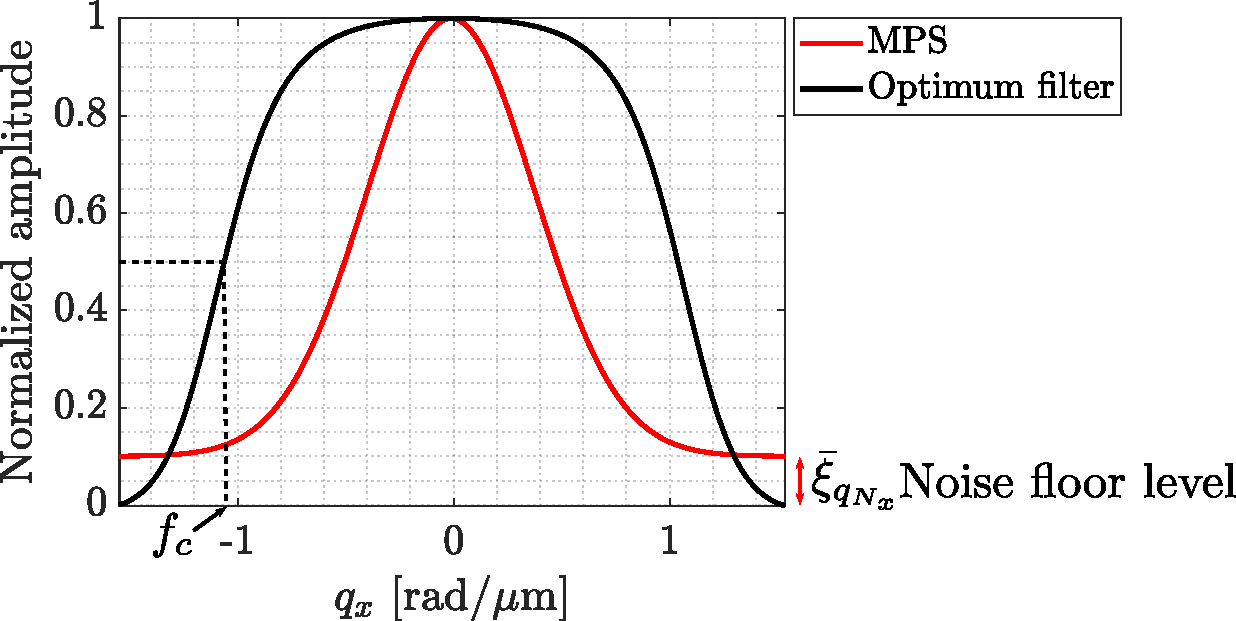
\includegraphics[width=.7\textwidth]{Figures/SHARP/OptimumFilterExample.pdf}
	\caption[Example of the optimum filter for a Gaussian MPS.]{Example of the optimum filter for a Gaussian MPS. $fc$: cutoff frequency of the filter.}
	\label{fig:OptimumFilter}
\end{figure}

Now that the phase stabilization and aberration correction procedures have been defined, the two 1D steps of SHARP can be condensed as
\begin{align}\label{eq:SHARP}
    \tilde{S}^{\text{1D}}(x,y,z) &= \mathbb{A}_x\left\{ \mathbb{C}_x\left\{ S(x,y,z) \right\} \right\}, \\
    \tilde{S}(x,y,z) &= \mathbb{A}_y\left\{ \mathbb{C}_y\left\{ \mathbb{C}^{-1}_x\left\{  \tilde{S}^{\text{1D}}(x,y,z) \right\} \right\} \right\},
\end{align}
where $\tilde{S}^{\text{1D}}(x,y,z)$ is the partially corrected tomogram and $\tilde{S}(x,y,z)$ is the $x$-$y$-separable aberrations corrected tomogram.

There are some particularities to discuss in regard to the described procedure. Because SHARP employs CAO, its operation is restricted to low-to-medium NA systems that is the regime of OCT. An extension to operate with high-NA systems could be possible by integrating ISAM in SHARP, however, this is the regime of OCM, which is not the aim in this work, and it is yet unclear whether ISAM procedure is compatible with 1D operation of SHARP.

The $x$-$y$ separability requirement has a direct limitation of the aberrations that can be corrected because not all aberrations can be separated into two 1D operations, only those whose deconvolution kernel can be separated into two 1D kernels. Among the $x$-$y$-separable aberrations, the most important for practical terms are defocus, $xy$-astigmatism and comma, being defocus the most relevant in many OCT applications given that it is intrinsic to the nature of the focused Gaussian beam used to illuminate the sample. In fact, defocus can be considered the only significant aberrations in many applications of OCT apart from retinal imaging where complex wavefronts may be induced by the eye of the subject. This means that SHARP is sufficient for many scenarios despite its $x$-$y$-separability requirement, in particular to numerically extend the depth of field, relaxing the trade-off between depth of field and lateral resolution.

Another important aspect is in regard to the role of the rollback step. The process of phase noise correction along the first axis adds random phase errors along the orthogonal axis that can become strong enough to frustrate the subsequent phase correction along the second axis, resulting in a lower local phase stability than the case of correcting the second axis directly, i.e. without correcting the first axis previously. The purpose of the RB step is to cancel out the first phase noise correction in order to avoid any strong error induced in the first correction. It can be noted that the RB step uses the phase noise correction computed before correcting aberrations along first axis but the RB itself is performed after correcting aberrations, which may change the phase pattern. Interestingly, the aberration correction applied along the first axis does not perturb the relative phase relation in the second axis although the phase pattern itself may have changed, hence the exact same phase noise correction is still valid for the RB (but conjugated) even though it is applied after aberration correction.

\section{Proof of concept experimental validation}\label{sec:Test}

To validate SHARP, an experiment was carried out in which a sample was imaged with a phase-unstable SSOCT system, inducing defocus on purpose by placing the focal plane of the scan lens outside the tissue thickness. A raster-scan non-$k$-clocked SSOCT system with a polygon-based wavelength-swept source was employed, similar to that in schematic Figure~\ref{fig:SSOCT_Scheme}. This custom-built system is affected by strong jitter in synchronization, as well as additional phase noise sources, such as the frequency shifter used to double the axial imaging range, that adds spurious phase offsets~\cite{Yun2004_Removing} and the galvo mirrors since the back-focal plane of the lens is not aligned with the pivot points of the galvos. The A-line repetition rate was $54$~kHz, in a $120$~nm $10$-dB-sweep spectral range centered at wavelength $1310$~nm. Light was focused onto the sample using a scan lens with transverse $e^{-2}$ beam diameter of $2w_0=22~\mu$m in a Rayleigh range of $z_R=290~\mu$m in air (Thorlabs LSM03, USA).

A \textit{cucumis sativus} sample was selected for the experiment as it displays prominent cellular walls with strong scattering, and large vacuoles with low scattering. The sample was imaged in a 3$\times$3~mm$^2$ lateral FoV within a ranging depth of 6~mm in air, acquiring 1024 samples per A-line, 512 A-lines per B-scan and 512 B-scans, for a total tomogram size of 1024$\times$512$\times$512 ($N_z\times N_x\times N_y$). A reference dataset was acquire placing the focal plane roughly 0.6~mm below the sample surface, referred to as \textit{in-focus} or reference tomogram, and the out-of-focus (OoF) dataset was acquired after shifting up the focal plane roughly 0.9~mm, thus located above the sample surface.

\begin{figure}[htb!]
	\centering
	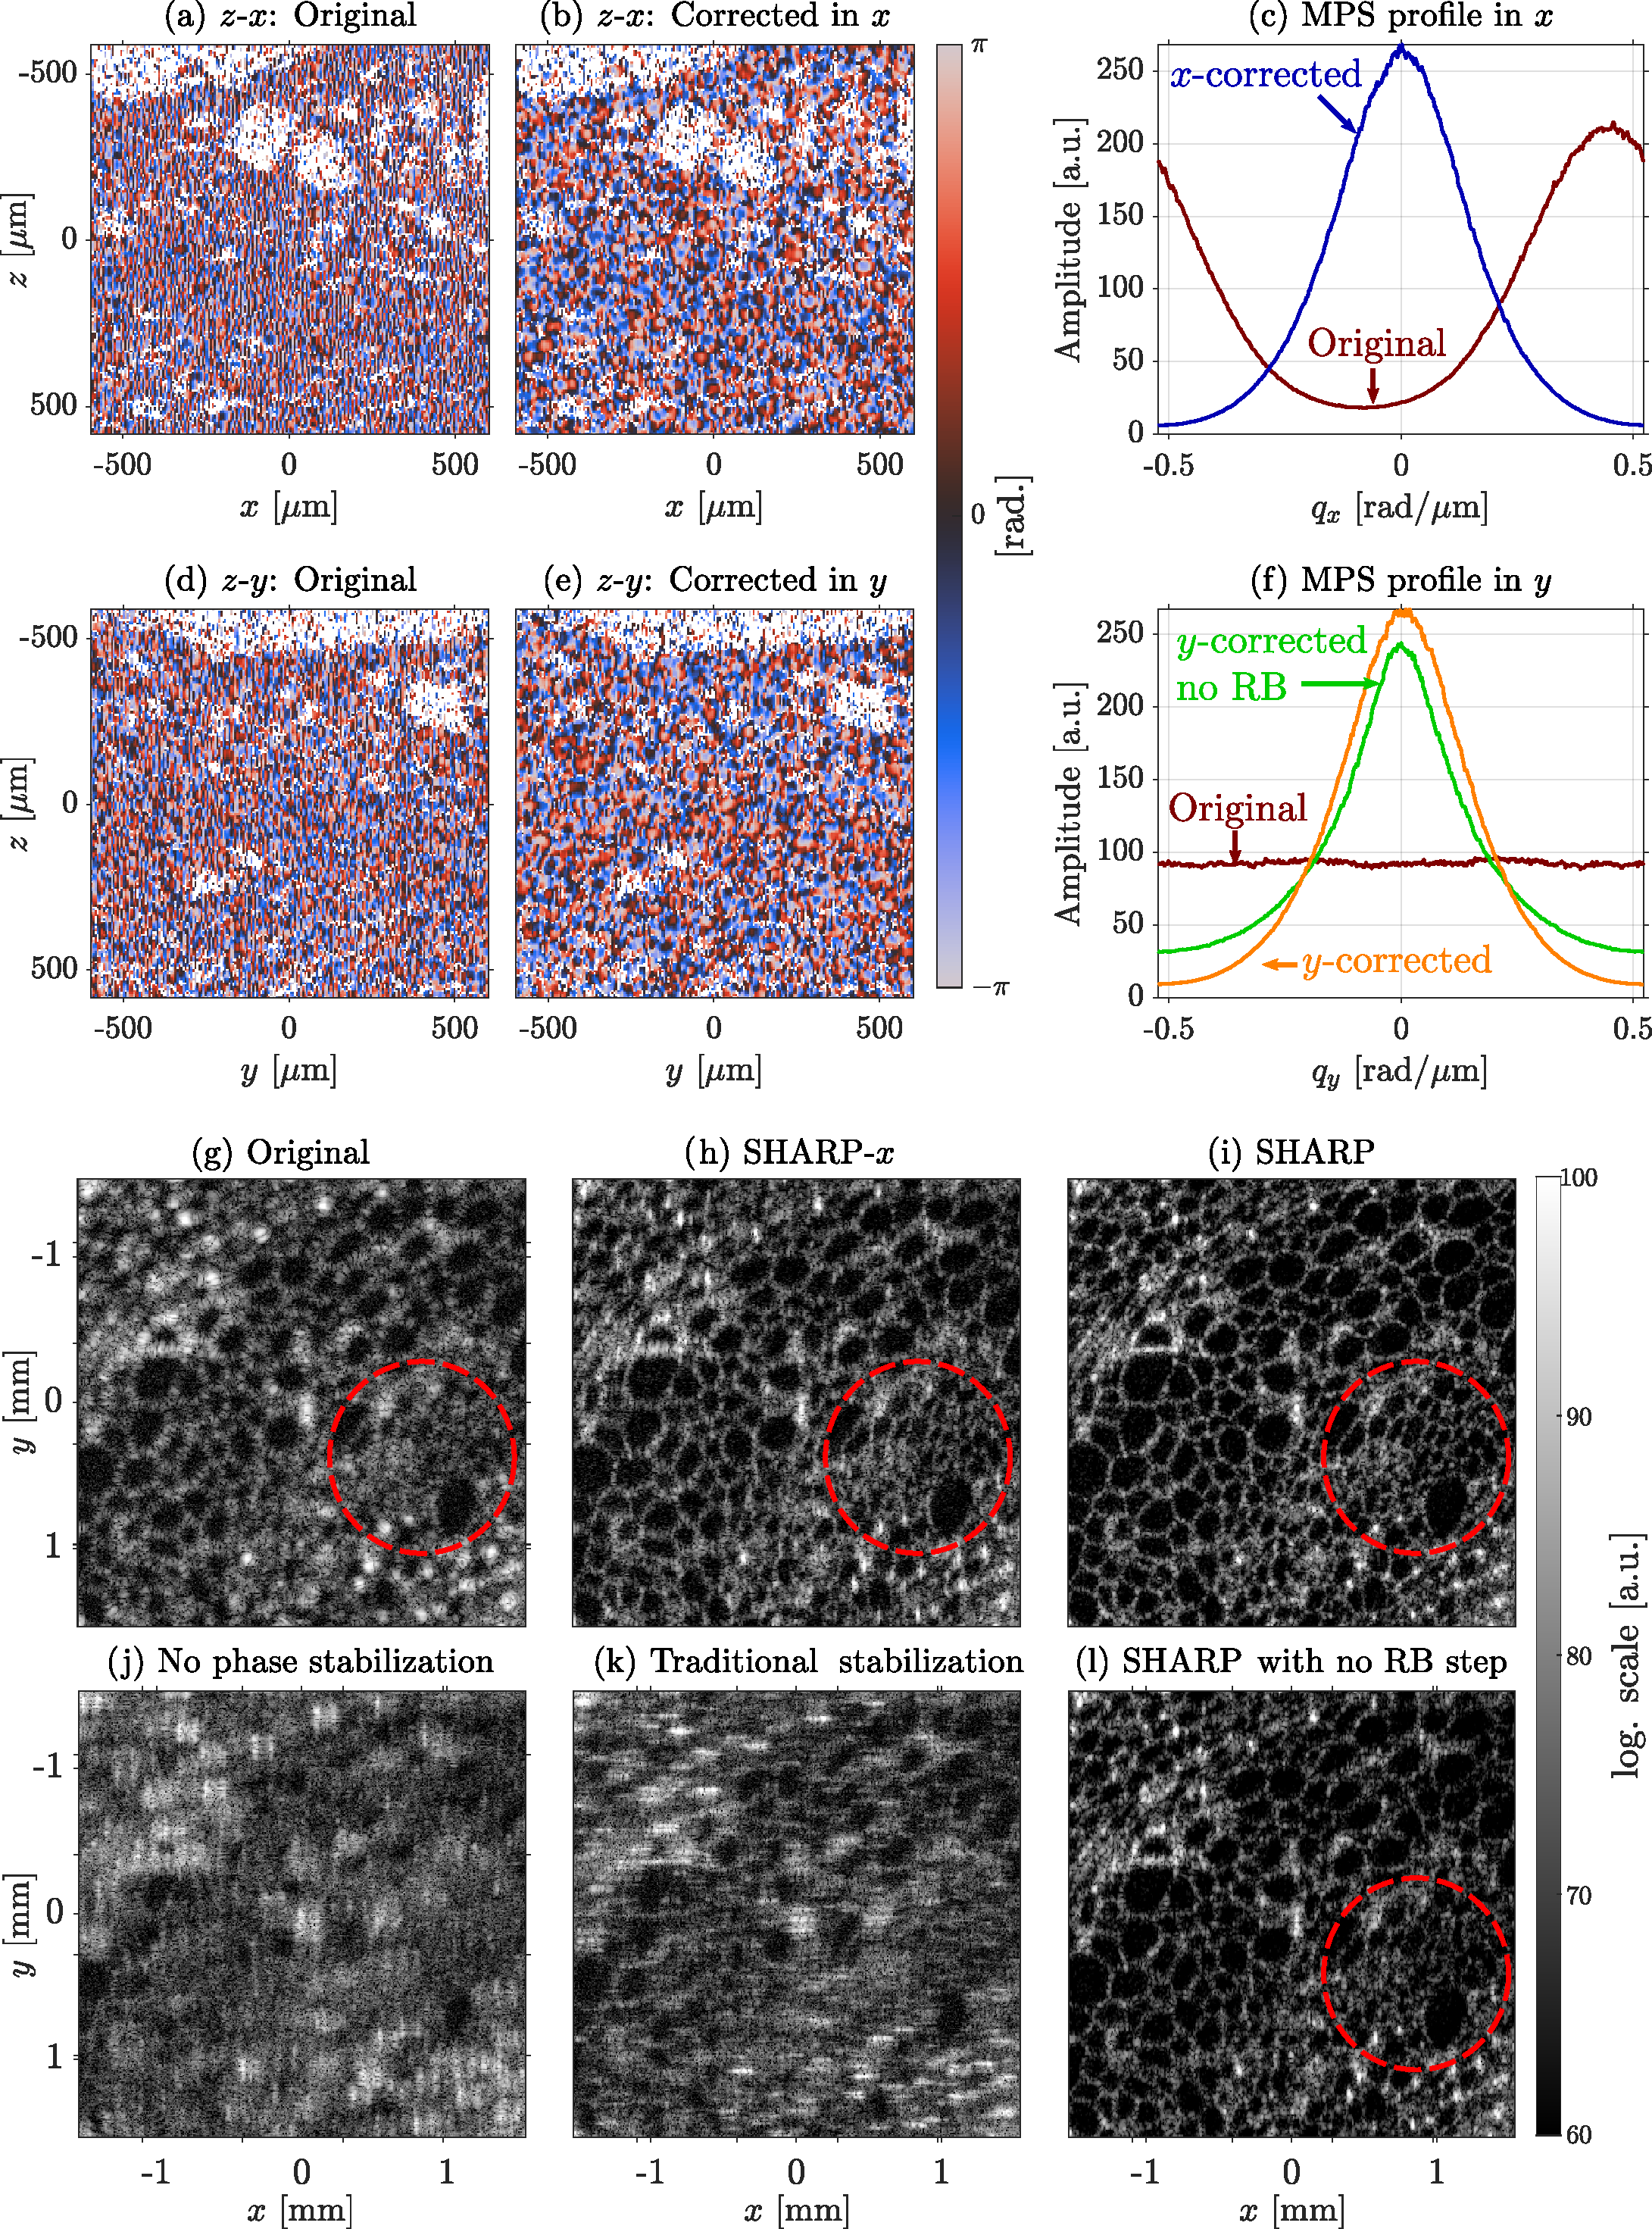
\includegraphics[width=.98\textwidth]{Figures/SHARP/SHARP_Cucumber.pdf}
	\caption[Proof of concept experimental validation of SHARP in a \textit{cucumis sativus} sample tomogram acquired with a SSOCT system.]{B-scan phase maps of \textit{cucumis sativus} sample in a small ROI; (a) before, (b) after $\mathbb{C}_x$ and (c) corresponding MPS profiles. $z$-$y$ phase maps; (d) before, (e) after $\mathbb{C}_y$ and (f) corresponding MPS profiles with and without RB step. Intensity \textit{en face} views; (g) original, (h) SHARP-$x$, (i)~SHARP, (l) SHARP without RB step, (j)~2D CAO with no phase stabilization and (k) with out-of-plane stabilization~\cite{Shemonski2014_Threedimensional}.}
	\label{fig:SHARP_Cucumber}
\end{figure}

SHARP was applied to the OoF tomogram using Legendre polynomial $P_2$ to describe the phase filter given that defocus is the only significant aberration in the experiment. Figure~\ref{fig:SHARP_Cucumber} illustrates results of each individual step of SHARP. A $z$-$x$ cross-sectional phase image in a small region of interest (ROI) of the raw unstable phase tomogram is shown in Fig.~\ref{fig:SHARP_Cucumber}(a), and after phase noise correction in $x$, or simply $\mathbb{C}_x$, in Fig.~\ref{fig:SHARP_Cucumber}(b), a point in which the MPS profile in $x$ exhibits a Gaussian shape and not a distorted one as original tomogram [Fig.~\ref{fig:SHARP_Cucumber}(c)]. After 1D CAO along $x$ axis (denoted as SHARP-$x$), the $zy$ plane remains phase unstable [Fig.~\ref{fig:SHARP_Cucumber}(d)], but after the RB step and $\mathbb{C}_y$, the $zy$ plane is now phase stable [Fig.~\ref{fig:SHARP_Cucumber}(d)] obtaining a MPS profile with Gaussian shape along $y$ [Fig.~\ref{fig:SHARP_Cucumber}(f)]. Without RB the MPS is distorted, approaching to a Gaussian function but with remnant high-frequency noise that suggests the presence of local phase instabilities that could frustrate CAO, as noted in the offset of green curve with respect to orange curve in Fig.~\ref{fig:SHARP_Cucumber}(f). Finally, a 2D refocused tomogram is obtained after applying 1D CAO in $y$.

Figures~\ref{fig:SHARP_Cucumber}(g)--(l) show intensity \textit{en face} views of the original tomogram, after SHARP-$x$ showing 1D refocusing only, after SHARP showing 2D refocusing and after SHARP without RB resulting in degraded quality of fine details, for instance in the region enclosed by the red circle, demonstrating the importance of the RB step. Additionally, results from failed attempts are illustrated; refocusing without any phase stabilization in Fig.~\ref{fig:SHARP_Cucumber}(j), showing destruction of signal information, and refocusing after phase stabilization only along out-of-plane axis in Fig.~\ref{fig:SHARP_Cucumber}(k), as is traditionally performed in SDOCT systems having in-plane phase stability~\cite{Shemonski2014_Threedimensional}, which also fails here because it is not sufficient for systems having 2D phase noise.

\begin{figure}[htb!]
	\centering
	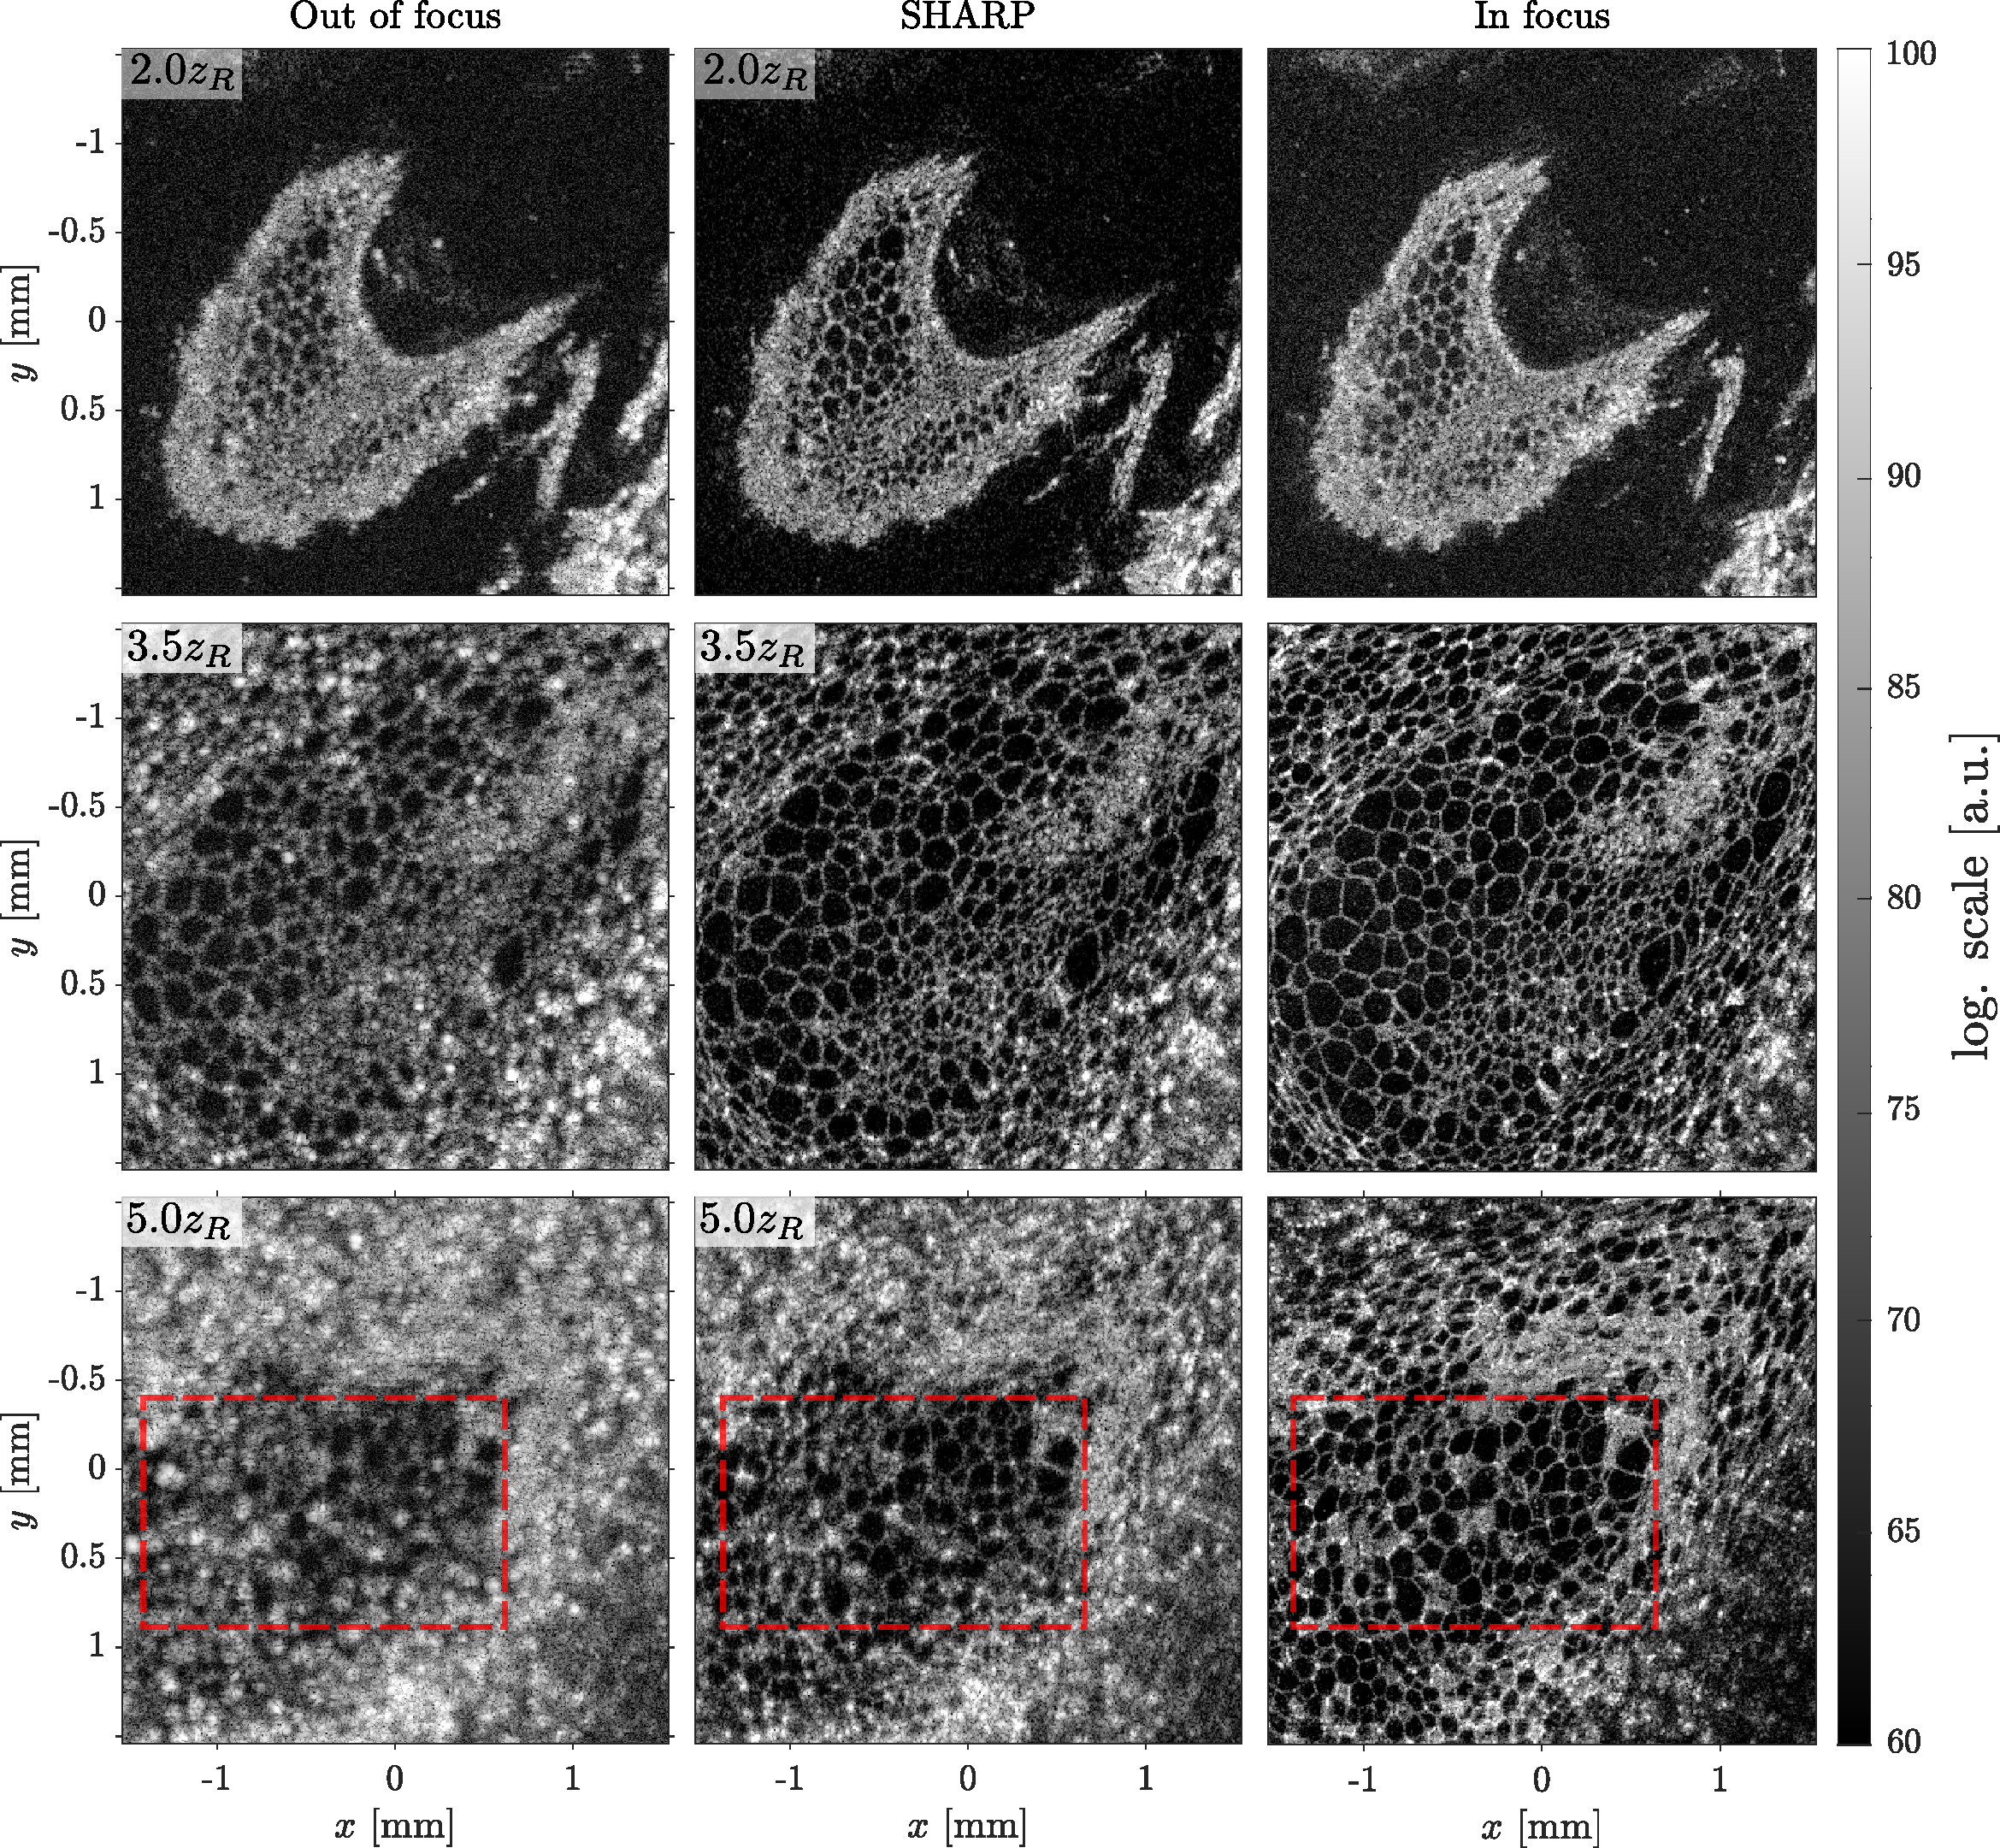
\includegraphics[width=\textwidth]{Figures/SHARP/SHARP_Cucumber_Enfaces.pdf}
	\caption[Comparison of several \textit{en face} views of out-of-focus, SHARP and in-focus tomograms.]{Comparison of several \textit{en face} views of out-of-focus, SHARP and in-focus tomograms, at depths $2.0z_R$, $3.5z_R$, and $5.0z_R$ as indicated in each image.}
	\label{fig:SHARP_CucumberEnfaces}
\end{figure}

Figure~\ref{fig:SHARP_CucumberEnfaces} presents \textit{en face} views located at depths $\sim 2.0z_R$, $3.5z_R$ and $5.0z_R$ from the focal plane of the OoF tomogram before and after SHARP, and of the corresponding in-focus reference tomogram. SHARP successfully restored the OoF tomogram despite the strong phase noise, providing images with better resolution and contrast than original images as a result of blurring correction and also due to the filtering effect of the optimum amplitude filter that reduced the average noise floor level from 63~dB to 59~dB, a difference corresponding to 1/10 of the images dynamic range 60--100~dB. In particular, cell walls of the sample are significantly sharper after SHARP compared to the original, approaching the in-focus counterparts, demonstrating the effectiveness of SHARP to correct for defocus.

For shallow depths, $2.0z_R$ and $3.5z_R$, SHARP produced successful results when compared to the reference images, but for the deepest plane shown, at $5.0z_R$, refocusing seems to be effective only for a small region having low signal density (see red boxes in Fig.~\ref{fig:SHARP_CucumberEnfaces}) whereas surrounding signal-dense region seems to be uncorrected. This may be a consequence of multiple scattering, which is likely to be stronger in these dense regions, and it is known that the deconvolution model only accounts for single-scattered or \textit{ballistic} photons, thus it is expected that a large contribution of multiple scattering hinders CAO, in this case for planes at $z>5.0z_R$ but this limit is sample-dependent.

SHARP was implemented in MATLAB and it took around 560~seconds to process the OoF tomogram in an ROI of size 450$\times$512$\times$512, using MATLAB 2019a in a workstation computer running on an Intel core i7-8700 processor @~3.2GHz. Aberration correction steps are the most computational expensive because of the optimization procedure performed in CAO, taking around 528 seconds for all planes including the two 1D corrections. In practical scenarios, it is possible to run the optimization only for certain planes and then to fit the optimal weights to find the correction for the intermediate planes, given that evolution of aberrations over depth is indeed smooth, and this will effectively reduce computation time.

\FloatBarrier

\section{Extending SHARP}\label{sec:Extensions}

\subsection{Complex amplitude motion artifacts correction}\label{sec:MotionCor}

Relevant effects of motion in the OCT signal for the context of CAC were already explain in Section~\ref{sec:phaseStab}, namely complex amplitude shift and phase-jump. The latter often has a greater relevance for CAC, thus phase stabilization methods correct phase offsets, including the phase stabilization performed in SHARP. However, in many \textit{in vivo} applications, complex amplitude shift may also have a significant influence and could be more noticeable since they affect both the phase and the amplitude of the tomogram, appearing as signal distortions in the structural image~\cite{Kraus2015_OCT}. In general, OCT systems are equipped with sample holders or interfaces to reduce impact of large acute motion, for instance chin rests and forehead holders in ophthalmic systems or handheld scanners for skin imaging, but there is yet low-frequency, slow motion arising from the heartbeat and respiration of the subject~\cite{Kraus2015_OCT}.

Motion artifacts can be prevented or corrected using a reference motion-free image from other imaging modality~\cite{Ricco2009_Correcting}, using tracking systems that follow and correct for sample motion \textit{in situ}, employed specially in retinal imaging~\cite{Maguluri2007_Three}, or using fast systems with volume acquisition rate such that sample appears static during the scanning, for instance recent reports have achieved volume acquisition rates in the order of tents of milliseconds with A-lines rates of the order of MHz~\cite{Auksorius2020_vivo}, but employing very specialized components. With A-line acquisition rates of the order of 100~kHz in current widespread systems, it is possible to assume that, in normal conditions, the sample is static during the acquisition of a single B-scan and motion manifests as rigid-body displacements across different B-scans, in other words, as inter-B-scan bulk displacements. In such case, complex amplitude shifts can be corrected straightforwardly using image registration~\cite{Zawadzki2007_Correction}.

The idea of bulk image registration is to find the relative global shift between two given images $I_1(m,l)$ and $I_2(m,l)$~\cite{Guizar-Sicairos2008_Efficient}. Most used method is intensity-based registration where the cross-correlation $r_{\text{cc}} = I_1(m,l)\star I_2(m,l)$ of the two images is computed and the location of the peak is found to determined the relative shift $(m_{\text{cc}}, l_{\text{cc}})$ between the two images, assuming that they are almost identical except for the relative shift between them. Then, the shift is applied to one of the two images in order to match one to the other. Commonly, cross-correlation is computed in Fourier domain as 
\begin{equation}\label{eq:ImageReg}
    r_{\text{cc}} = \text{FT}^{-1}_{q_m,q_l}\left\{\text{FT}_{m,l}\left\{I_1(m,l)\right\}\text{FT}_{m,l}\left\{I_2(m,l)\right\}^\ast\right\},
\end{equation}
where $^\ast$ denotes complex conjugate, then the shift is corrected as
\begin{equation}
    I_2 = \text{FT}^{-1}_{q_m,q_l}\left\{\text{FT}_{m,l}\left\{I_2(m,l)\right\} \exp\left[-i2\pi\left(m_{\text{cc}} \frac{q_m}{M} + l_{\text{cc}} \frac{q_l}{L}\right)\right]\right\},
\end{equation}
where $m_{\text{cc}}$ and $l_{\text{cc}}$ are given in pixels and $M\times L$ is the image size.

When a sub-pixel estimation is required, the product of the two Fourier-transformed images in Eq.~\eqref{eq:ImageReg} is zero-padded prior to computation of the inverse FT in order to have an upsampled cross-correlation $r_{\text{cc}}$. However, this zero-padding will increase the size of the input of the inverse FT increasing computational cost significantly as the sub-pixel resolution increases, for instance a $1/20$ resolution requires a zero-padding of $20M\times 20L$. Fortunately, there are efficient sub-pixel image registration methods that significantly improve speed without sacrificing accuracy~\cite{Guizar-Sicairos2008_Efficient}.

Using efficient sub-pixel image registration, it is possible to include a step for inter-B-scan bulk motion correction in SHARP procedure, assuming that transitions between B-scans is smooth, which is valid for typical biological samples scanned with a proper sampling, ideally equal or better than Nyquist sampling. This step, if necessary, is performed after the first phase stabilization step since correcting the complex signal requires phase stable data. Complex-shifts correction could enable operation of subsequent steps of SHARP for \textit{in vivo} imaging. Motion is corrected in SHARP by registering intensity of adjacent B-scans $n$ and $n-1$ and finding the relative lateral and axial shifts $(m_\text{cc}(n), l_\text{cc}(n))$ as
\begin{equation}
    (m_\text{cc}(n), l_\text{cc}(n)) = \arg\left\{\max\left\{ |S(m,n,l)|^2\star |S(m,n-1,l)|^2 \right\}\right\},
\end{equation}
where the cross-correlation is performed inside the B-scan plane, i.e. along coordinates $x$ and $z$. Shifts across B-scans are accumulated to computed global shifts with respect to the first B-scan as
\begin{equation}
    \mu_{\text{cc}}(n) = \sum_{\hat{n}}^n m_{\text{cc}}(\hat{n}) \ \ \ \ \ \text{and} \ \ \ \ \  \Gamma_{\text{cc}}(n) = \sum_{\hat{n}}^n l_{\text{cc}}(\hat{n}),
\end{equation}
that are applied to obtain a bulk motion-corrected complex tomogram $S_\text{mc}(m,n,l)$,
\begin{equation}
    S_\text{mc}(m,n,l) = \text{FT}^{-1}_{q_m,q_l}\left\{\text{FT}_{m,l}\left\{S(m,n,l)\right\} \exp\left[-i2\pi\left( \mu_{\text{cc}}(n)\frac{q_m}{M} + \Gamma_{\text{cc}}(n)\frac{q_l}{L}\right)\right]\right\}.
\end{equation}

Additionally, global shifts can be high-pass filtered to cancel out the spurious low-frequency shifts that appear when the sample has a non-flat geometry, for instance the curvature of the cornea, in order to preserv the surface geometry of the sample.

With this motion correction step, it could be possible to correct $x$-$y$-separable aberrations with SHARP in tomograms acquired \textit{in vivo} affected by bulk motion subject to the B-scan plane (inter-B-scan), but insignificant out-of-plane motion (intra-B-scan) since it is not addressed in the approach described above, actually out-of-plane corrections demands more sophisticated solutions out of the scope here~\cite{Kraus2012_Motion}. To register B-scans, the efficient sub-pixel image registration by cross-correlation algorithm~\cite{Guizar-Sicairos2008_Efficient} is used here, available in \href{https://www.mathworks.com/matlabcentral/fileexchange/18401-efficient-subpixel-image-registration-by-cross-correlation}{MATLAB Central File Exchange}~\cite{Guizar2020_Efficient}.

Figure~\ref{fig:MotionCor} illustrates motion correction with the simulated OCT tomogram used in previous demonstrations. Global lateral and axial shifts were defined randomly for each B-scan and applied to the original motion-free tomogram, then the motion correction procedure was carried out to compensate for the induced shifts using a sub-pixel resolution of $1/20$. Figs.~\ref{fig:MotionCor}(a)-(c) compare \textit{en face} views of each tomogram, and the effect of inter-B-scan bulk motion can be visualized in Fig.~\ref{fig:MotionCor}(b) as distortions and discontinuities along the $y$ axis. This is also evident comparing the cross-sectional $z$-$y$ planes in Figs.~\ref{fig:MotionCor}(d)-(f). In both views, it is clear that the motion correction yields a tomogram with no perceptual artifacts, approaching the appearance of the original one. In Fig.~\ref{fig:MotionCor}(g), a zoomed region of the cross-correlation image between two B-scan with relative shift of 3 pixels is shown, to illustrate how the location of the peak is shifted from the center of the image, indicating the relative displacement. 

\begin{figure}[htb!]
	\centering
	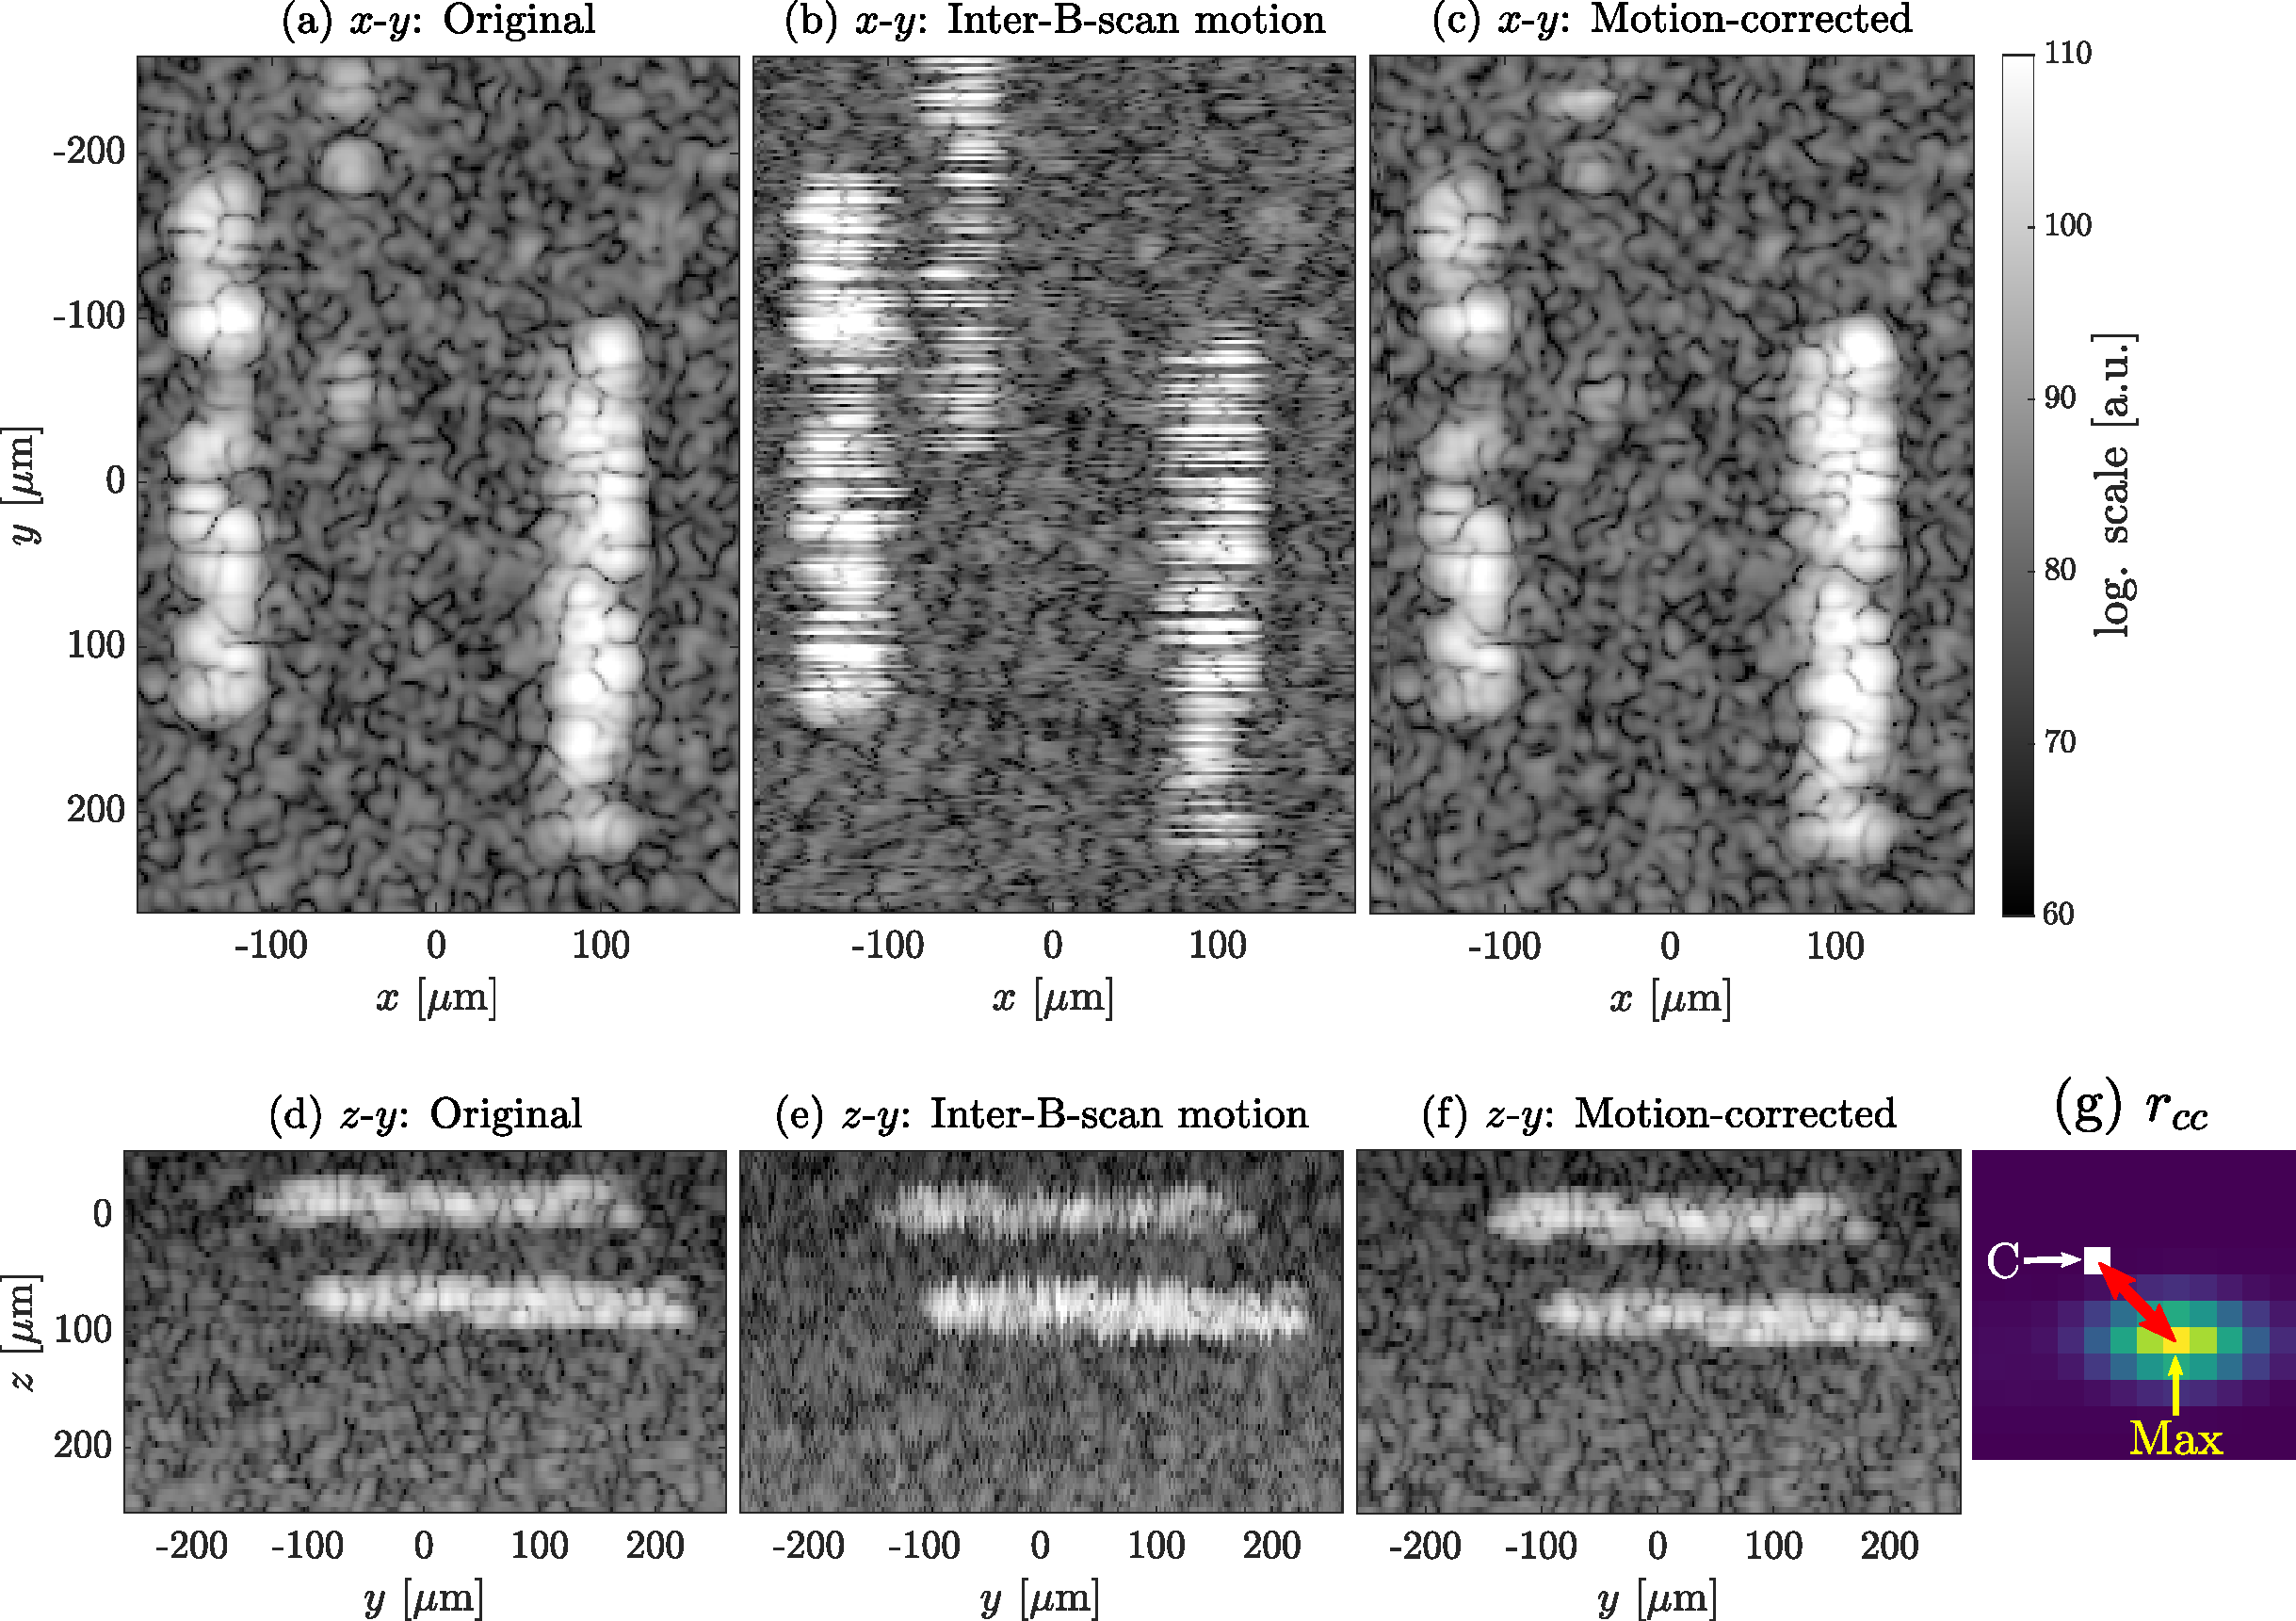
\includegraphics[width=\textwidth]{Figures/SHARP/MotionCorrection.pdf}
	\caption[Illustration of intra-B-scan motion correction with a simulated OCT tomogram.]{Illustration of intra-B-scan motion correction with a simulated OCT tomogram. (a), (d) original; (b), (e) original with induced axial and lateral in-plane bulk motion; (c), (f) motion corrected using image registration. (a)-(c) are \text{en-face} views and (d)-(f) are cross-sections of $z$-$y$ plane. (g) Example of the cross-correlation between two B-scan with relative motion (not shown). C: center pixel, Max: location of the maximum value of the cross-correlation. Red arrow indicates the estimated shift between the two B-scans.}
	\label{fig:MotionCor}
\end{figure}
\FloatBarrier

\subsection{Spatially-varying aberrations correction}

Although the numerical deconvolution in CAO is performed in Fourier domain for practical simplicity, by applying a complex filter to each \textit{en face} plane, the physical convolution in the image formation process actually occurs in spatial domain. The possibility to perform the numerical deconvolution in Fourier domain relies on the fact that the deconvolution kernel in spatial domain is constant over the lateral field of view (FoV) ---not to be confused with axial depth of field.--- The region within this assumption is valid is known as the \textit{isoplanatic-patch}, a term originated from astronomy~\cite{Beckers1993_Adaptive}, defined as the region within which aberrations and therefore the point spread function (PSF) do not vary~\cite{Kumar2015_Anisotropic}. There are scenarios where the lateral FoV is greater than the isoplanatic-patch, consequently the PSF is anisotropic resulting in aberrations that vary across the FoV thus they cannot be corrected entirely using a global filter in Fourier domain.  For instance, it is known that large numerical aperture systems often have a small diffraction-limited lateral FoV and outside this the resolution degrades progressively. Additional causes of an anisotropic PSF may be imperfect optical components, misalignment, or inhomogeneous samples, for instance in corneal imaging, where the axial focal position is not longer constant forming a plane, instead it is curved as a consequence of cornea curvature.

In rigorous terms, spatial-varying aberrations must be corrected locally, using a deconvolution kernel defined individually at each spatial coordinate. This would be computationally expensive and a fully localized correction might not be necessary for certain practical scenarios because variation of aberrations across the FoV is indeed smooth. To deal with spatial-varying aberration, region of interest-based CAO have been proposed for sub-aperture-based and optimization-based CAO~\cite{Kumar2015_Anisotropic, South2019_Local} under the general idea of splitting the FoV into several regions of interests (ROIs) or windows to perform CAO individually in each ROI and then stitching the aberration-corrected ROIs into the original full FoV. Ideally, aberrations within each ROI should be nearly constant, this is achievable using small ROIs, but in practice there is a limit on the minimum size given that the determination of aberrations in the CAO procedure could fail if few pixels are used.

Based on former idea, it is possible to perform spatially-varying aberration correction in SHARP procedure, as is illustrated in Figure~\ref{fig:spatialAber}, instead of using the standard global aberration correction. To do so, each \textit{en face} plane is splitted into windows of size $W_x\times W_y$ with an overlap of half window size along the axis being corrected, for instance, an overlap of $W_x/2\times 0$ when correcting in $x$ axis, or $0\times W_y/2$ for $y$ axis. Given the 1D operation of SHARP, overlap is not necessary in the axis that is not the interest in each aberration-correction step. The purpose of overlapping the windows is to avoid boundaries artifacts that appear in the composite images when there is not overlap. After performing CAO in each window, full \textit{en face} planes are assembled extracting an centered ROI of size $W_x/2\times W_y$  from each window when correcting along $x$, or $W_x\times W_y/2$ when correcting along $y$ axis. For windows occupying the frontier of the full image in the axis of interest (red box in Fig.~\ref{fig:spatialAber}), an extended ROI is selected in order to keep the same full image size. The appropriate number of windows may change for every tomogram depending on the sample and the anisotropy of aberrations.

\begin{figure}[htb!]
	\centering
	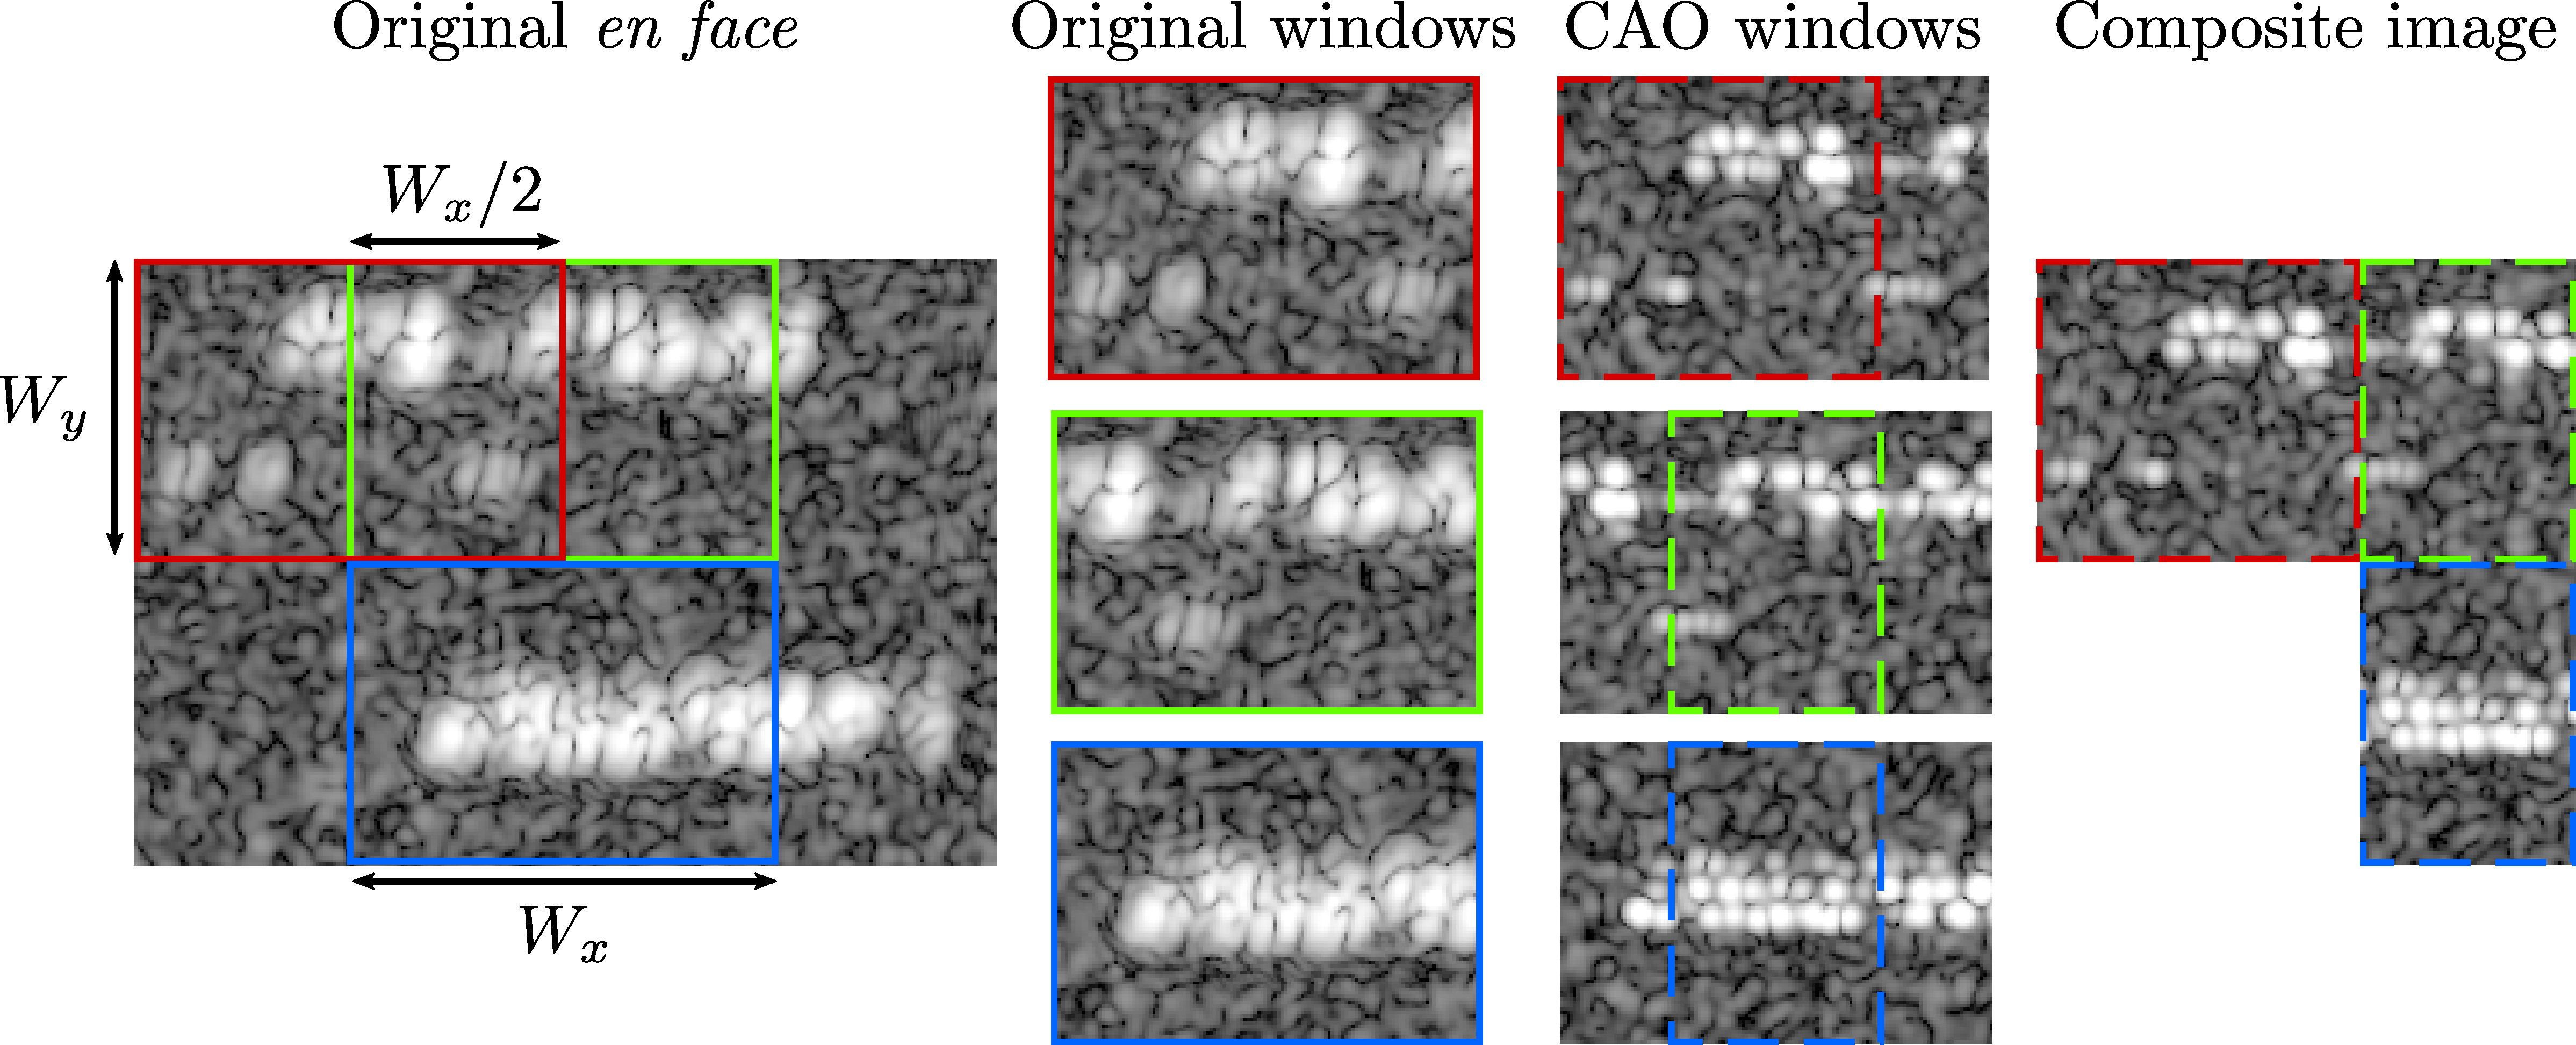
\includegraphics[width=\textwidth]{Figures/SHARP/SpatialVarAber.pdf}
	\caption[Illustration of spatially-varying aberration correction with a simulated OCT \textit{en face}.]{Illustration of spatially-varying aberration correction with a simulated OCT \textit{en face}, showing the process for three windows only to facilitate interpretation.}
	\label{fig:spatialAber}
\end{figure}


\FloatBarrier

\subsection[Beyond correction of separable in \textit{x-y} aberrations]{Beyond correction of separable in $x$-$y$ aberrations}

Although SHARP is capable of correcting for defocus and $xy$-astigmatism, the two major aberrations in OCT for many applications, a clear drawback is the constrain to only correct for $x$-$y$-separable aberrations, and this could limit applicability of SHARP, in particular, in retinal imaging applications given that arbitrary aberrations are present depending on the subject's eye~\cite{Kumar2017_Invivo, Ginner2018_Holographic, Hillmann2016_Aberrationfree}, It is therefore desirable to extend the procedure to cover more general aberrations and expand its applicability throughout more practical scenarios.

In the standard or SHARP-$xy$ procedure, aberrations are corrected along the two main axes $x$ and $y$. Keeping in mind the 1D operation, it is possible to correct aberrations along two secondary axes $x'$ and $y'$ obtained as the original axes $x$ and $y$ rotated by 45 degrees with the relationships $x'=x\cos45^\circ - y\sin45^\circ$ and $y' = x\sin45^\circ + y\cos45^\circ$. In principle, correcting for aberrations in the axes $x$-$y$ and then in the axes $x'$-$y'$ provides a global correction of aberrations oriented at an arbitrary angle. For instance, SHARP-$xy$ and SHARP-$x'y'$ can correct for $xy$- and oblique-astigmatism respectively, then complementing both procedures, it is possible to correct for astigmatism oriented at an arbitrary angle obtained from a combination of the two independent astigmatisms. 

The procedure for SHARP-$x'y'$ follows the idea behind the simple steps of the original method with slight differences as explain next and illustrated in Figure~\ref{fig:SHARP45d_Diag} for a grid of $6\times 6$ pixels. Local phase differences $\delta(m,n)$ for phase noise correction are computed between consecutive A-lines oriented in oblique paths [red lines in Fig.~\ref{fig:SHARP45d_Diag}(b)], denoted by indexes $(m,n)$ and $(m-1, n+1)$ in the case of correcting along $x'$ axis or $(m,n)$ and $(m+1, n-1)$ when correcting along $y'$ axis, then the proper accumulative sum is performed and this way phase stability is achievable along any oblique axis, $x'$ or $y'$. After phase stabilization, it is now possible to perform aberration correction along the phase-stable oblique axis.

\begin{figure}[htb!]
	\centering
	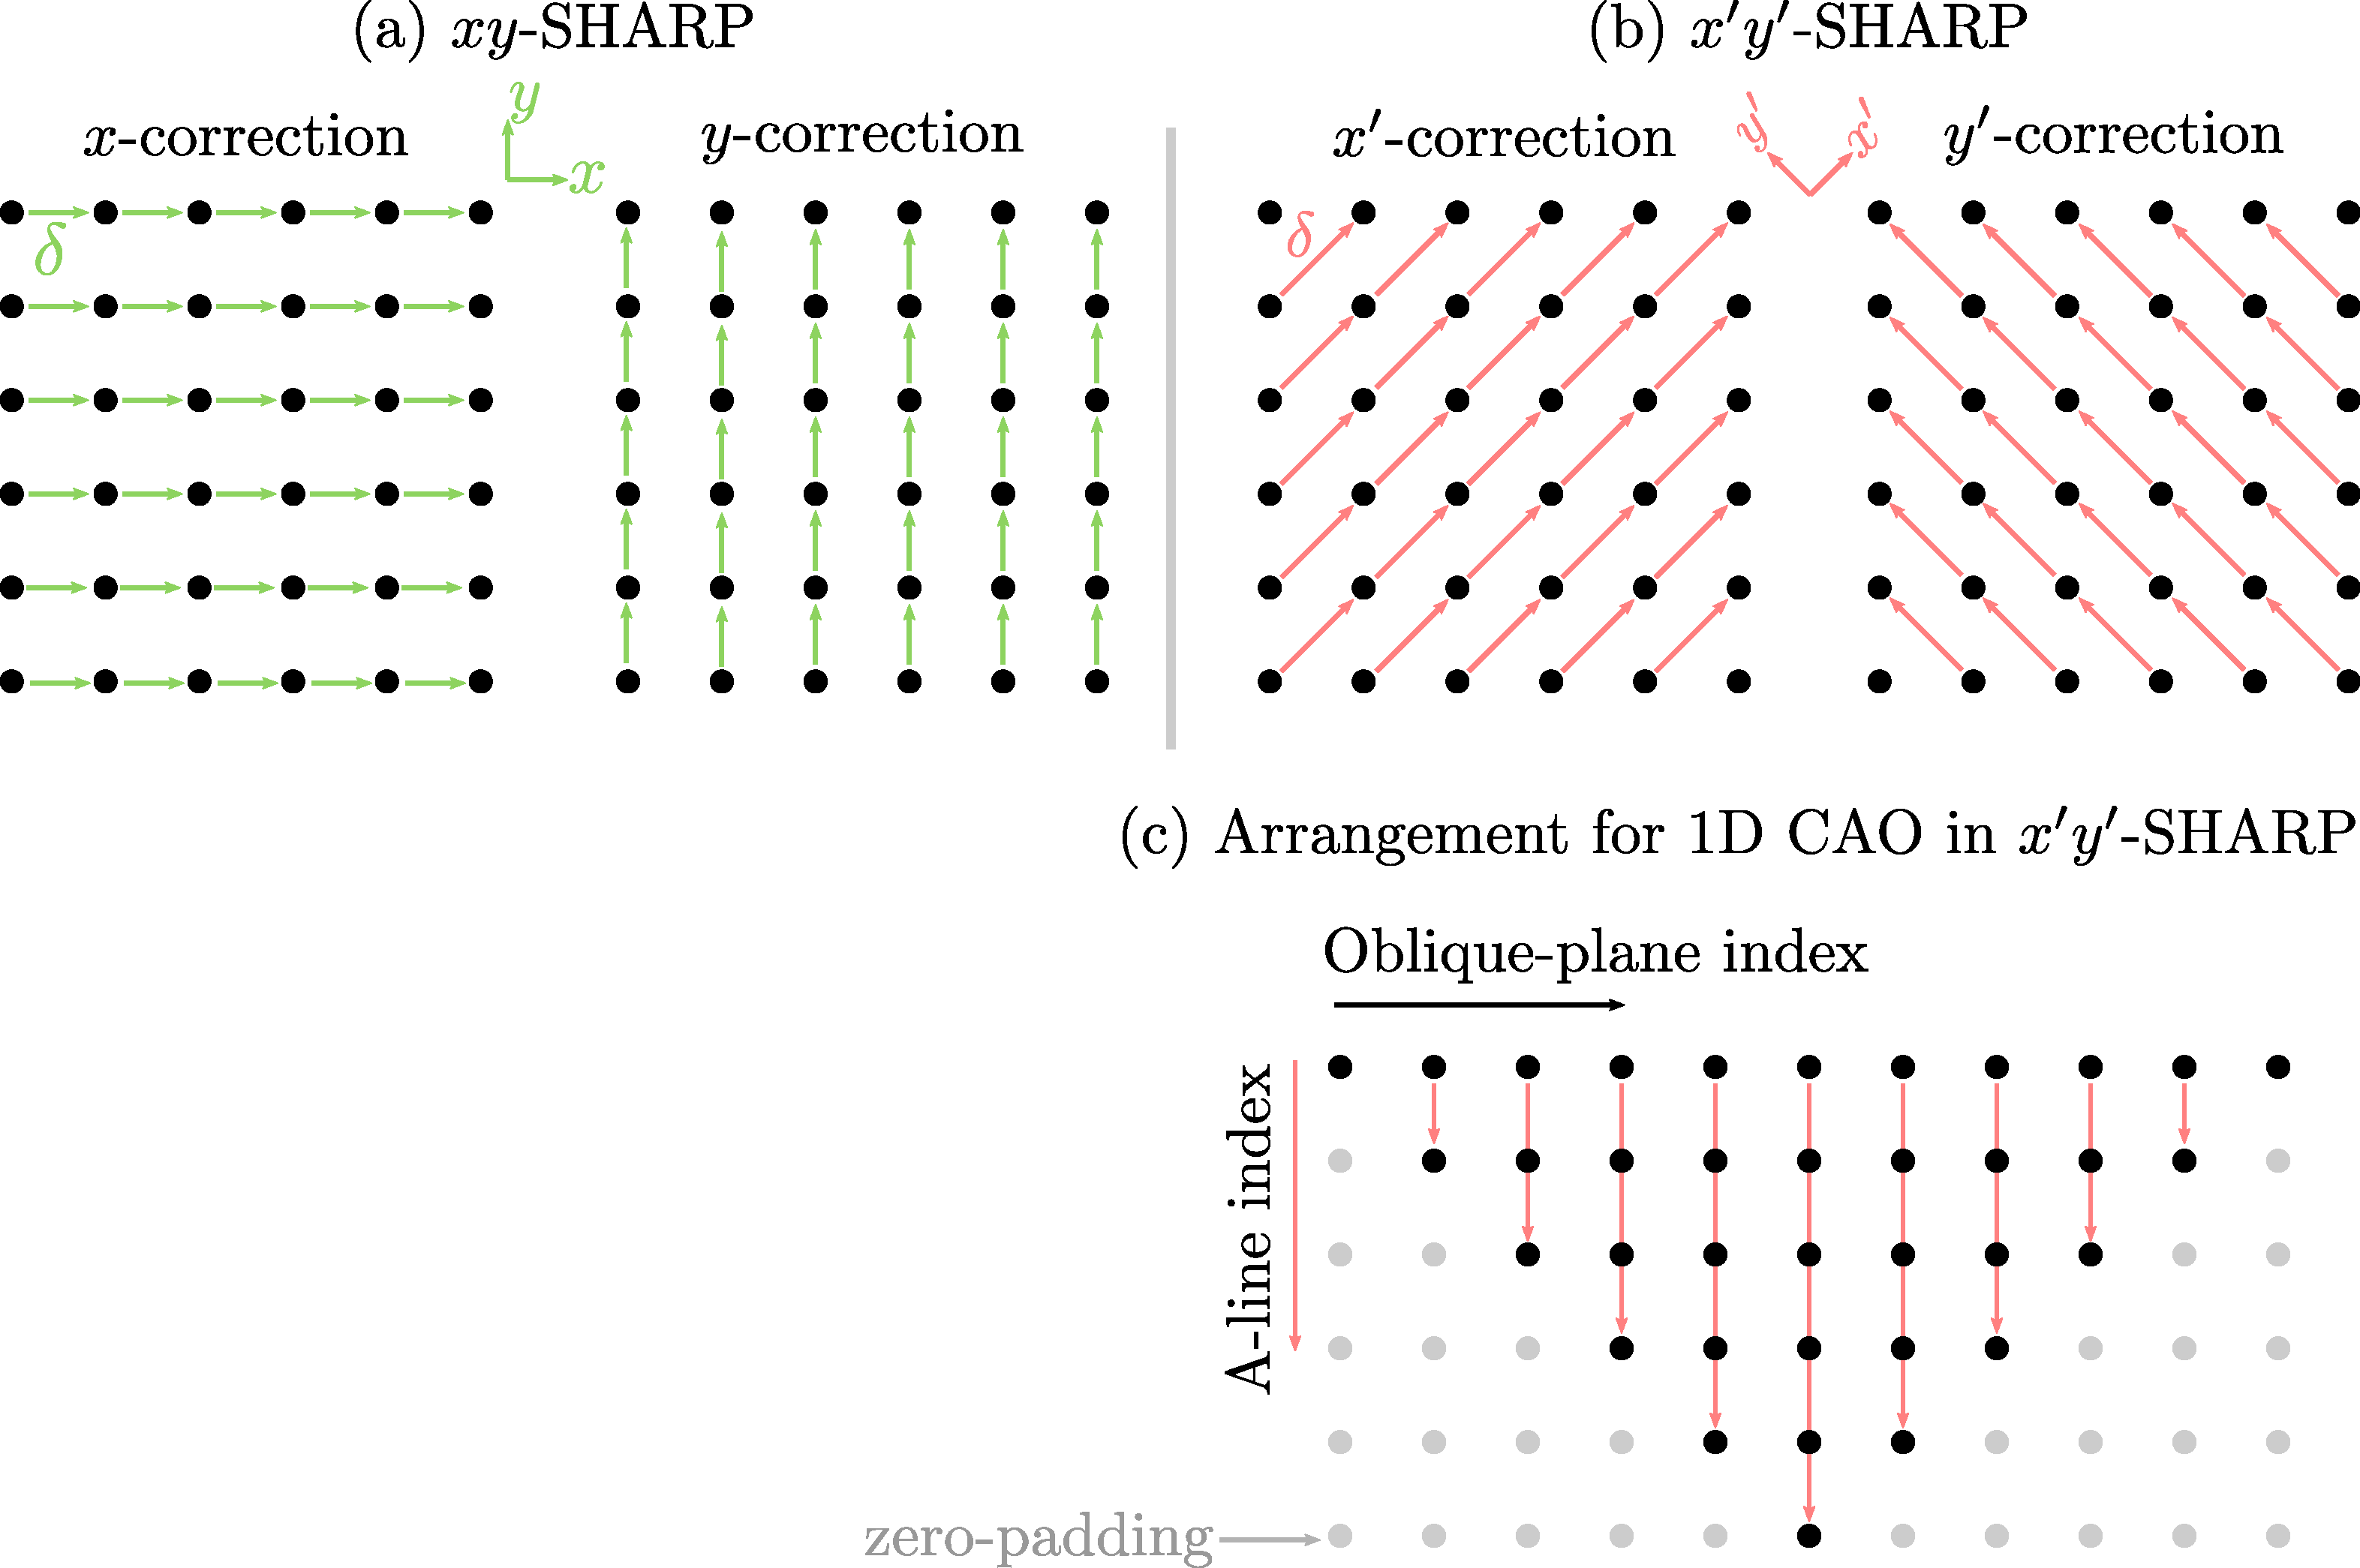
\includegraphics[width=\textwidth]{Figures/SHARP/SHARP45d_Diagram.pdf}
	\caption[Comparison of operation of SHARP-$xy$ and SHARP-$x'y'$.]{Comparison of operation of SHARP-$xy$ and SHARP-$x'y'$ for a grid of $6\times 6$ pixels. (a) Phase differences in SHARP-$xy$ are computed along vertical and horizontal paths, whereas (b) for SHARP-$x'y'$ are computed along oblique paths. (c) The tomogram grid is rearranged in order to perform CAO along an oblique axes.}
	\label{fig:SHARP45d_Diag}
\end{figure}

The essence of 1D CAO for the oblique axes is the same as that for the main axes but there are changes in the numerical implementation in order to carry out the corresponding calculations.  In a standard tomogram, \textit{en face} plane is arranged with one dimension being A-line index ($x$ axis) and the other being B-scan plane index ($y$ axis). To carry out 1D CAO in SHARP-$x'y'$, the tomogram is rearranged in the \textit{en face} plane in such way that one dimension corresponds to the A-line index ($x'$ axis) and the other to the oblique-plane index ($y'$ axis) [see Fig,~\ref{fig:SHARP45d_Diag}(c)]. In addition, the rearranged tomogram is zero-padded to keep a constant oblique-plane size because original planes have different numbers of A-lines. Then, the standard 1D CAO procedure can be applied directly to the rearranged tomogram using the A-line index dimension as the aimed dimension for the calculations.

The zero-padding in the rearrangement step provides a tomogram with uniform size, but it is clear that the number of A-lines with effective (non-zero) information in each oblique-plane is different, and it approaches to one A-line towards the tomogram frontiers. Because of that, planes having less A-lines than the deconvolution kernel size will possibly end up with a wrong correction, however, this effect is unimportant given that it occurs only towards the corners  of the FoV.

Because phase differences for noise correction in SHARP-$x'y'$ are computed between A-lines separated by $\sqrt{2}$ times the lateral sampling (and not by exactly the lateral sampling as in SHARP-$xy$), then in order to fulfill sampling requirement for CAO, the effective sampling of the tomogram should be $1/\sqrt{2}$ times the Nyquist sampling, i.e. $\delta_x/(2\sqrt{2})$, or smaller, this means that a finer lateral sampling is required. This is a key aspect to keep in mind but it does not have important experimental consequences given that in most systems sampling can be adjusted.

In the case of performing SHARP-$x'y'$ after applying SHARP-$xy$, it is important to rollback the last phase noise correction after the second aberration correction of  SHARP-$xy$, otherwise, subsequent phase noise corrections are likely to fail. In general, the entire SHARP procedure would consist in four steps, each one performing a phase noise and aberration correction along a single axis at a time, connected by their corresponding rollback step. An intuitive order for the axis of interest is each step is first $x$, then $y$, then $x'$ and finally $y'$, although order can be changed indistinctly.

A preliminary test using the simulated OCT tomogram mentioned previously was carried out to verify the correct operation of SHARP-$x'y'$ and results are summarized in Fig.~\ref{fig:SHARP45d_Int}. To establish a reference for comparison, intrinsic defocus of the tomogram was corrected using 2D CAO. Aberrations were induced in the original tomogram by applying a phase filter created with Zernike polynomials $Z_4$ and $Z_5$ for $xy$- and oblique-astigmatism with weights $0.8\lambda$ and $2.4\lambda$ respectively. Figs.~\ref{fig:SHARP45d_Int}(a) and (b) show one \textit{en face} plane of the aberration-free and aberrated tomograms. Fig.~\ref{fig:SHARP45d_Int}(e) shows the aberration wavefront exhibiting astigmatism oriented at an arbitrary angle, but close to 45 degrees given that the magnitude of the weight of $Z_5$ is greater, and it also shows the aberrated wavefront for the \textit{en face} plane Figs.~\ref{fig:SHARP45d_Int}(b) including its intrinsic defocus. 

\begin{figure}[htb!]
	\centering
	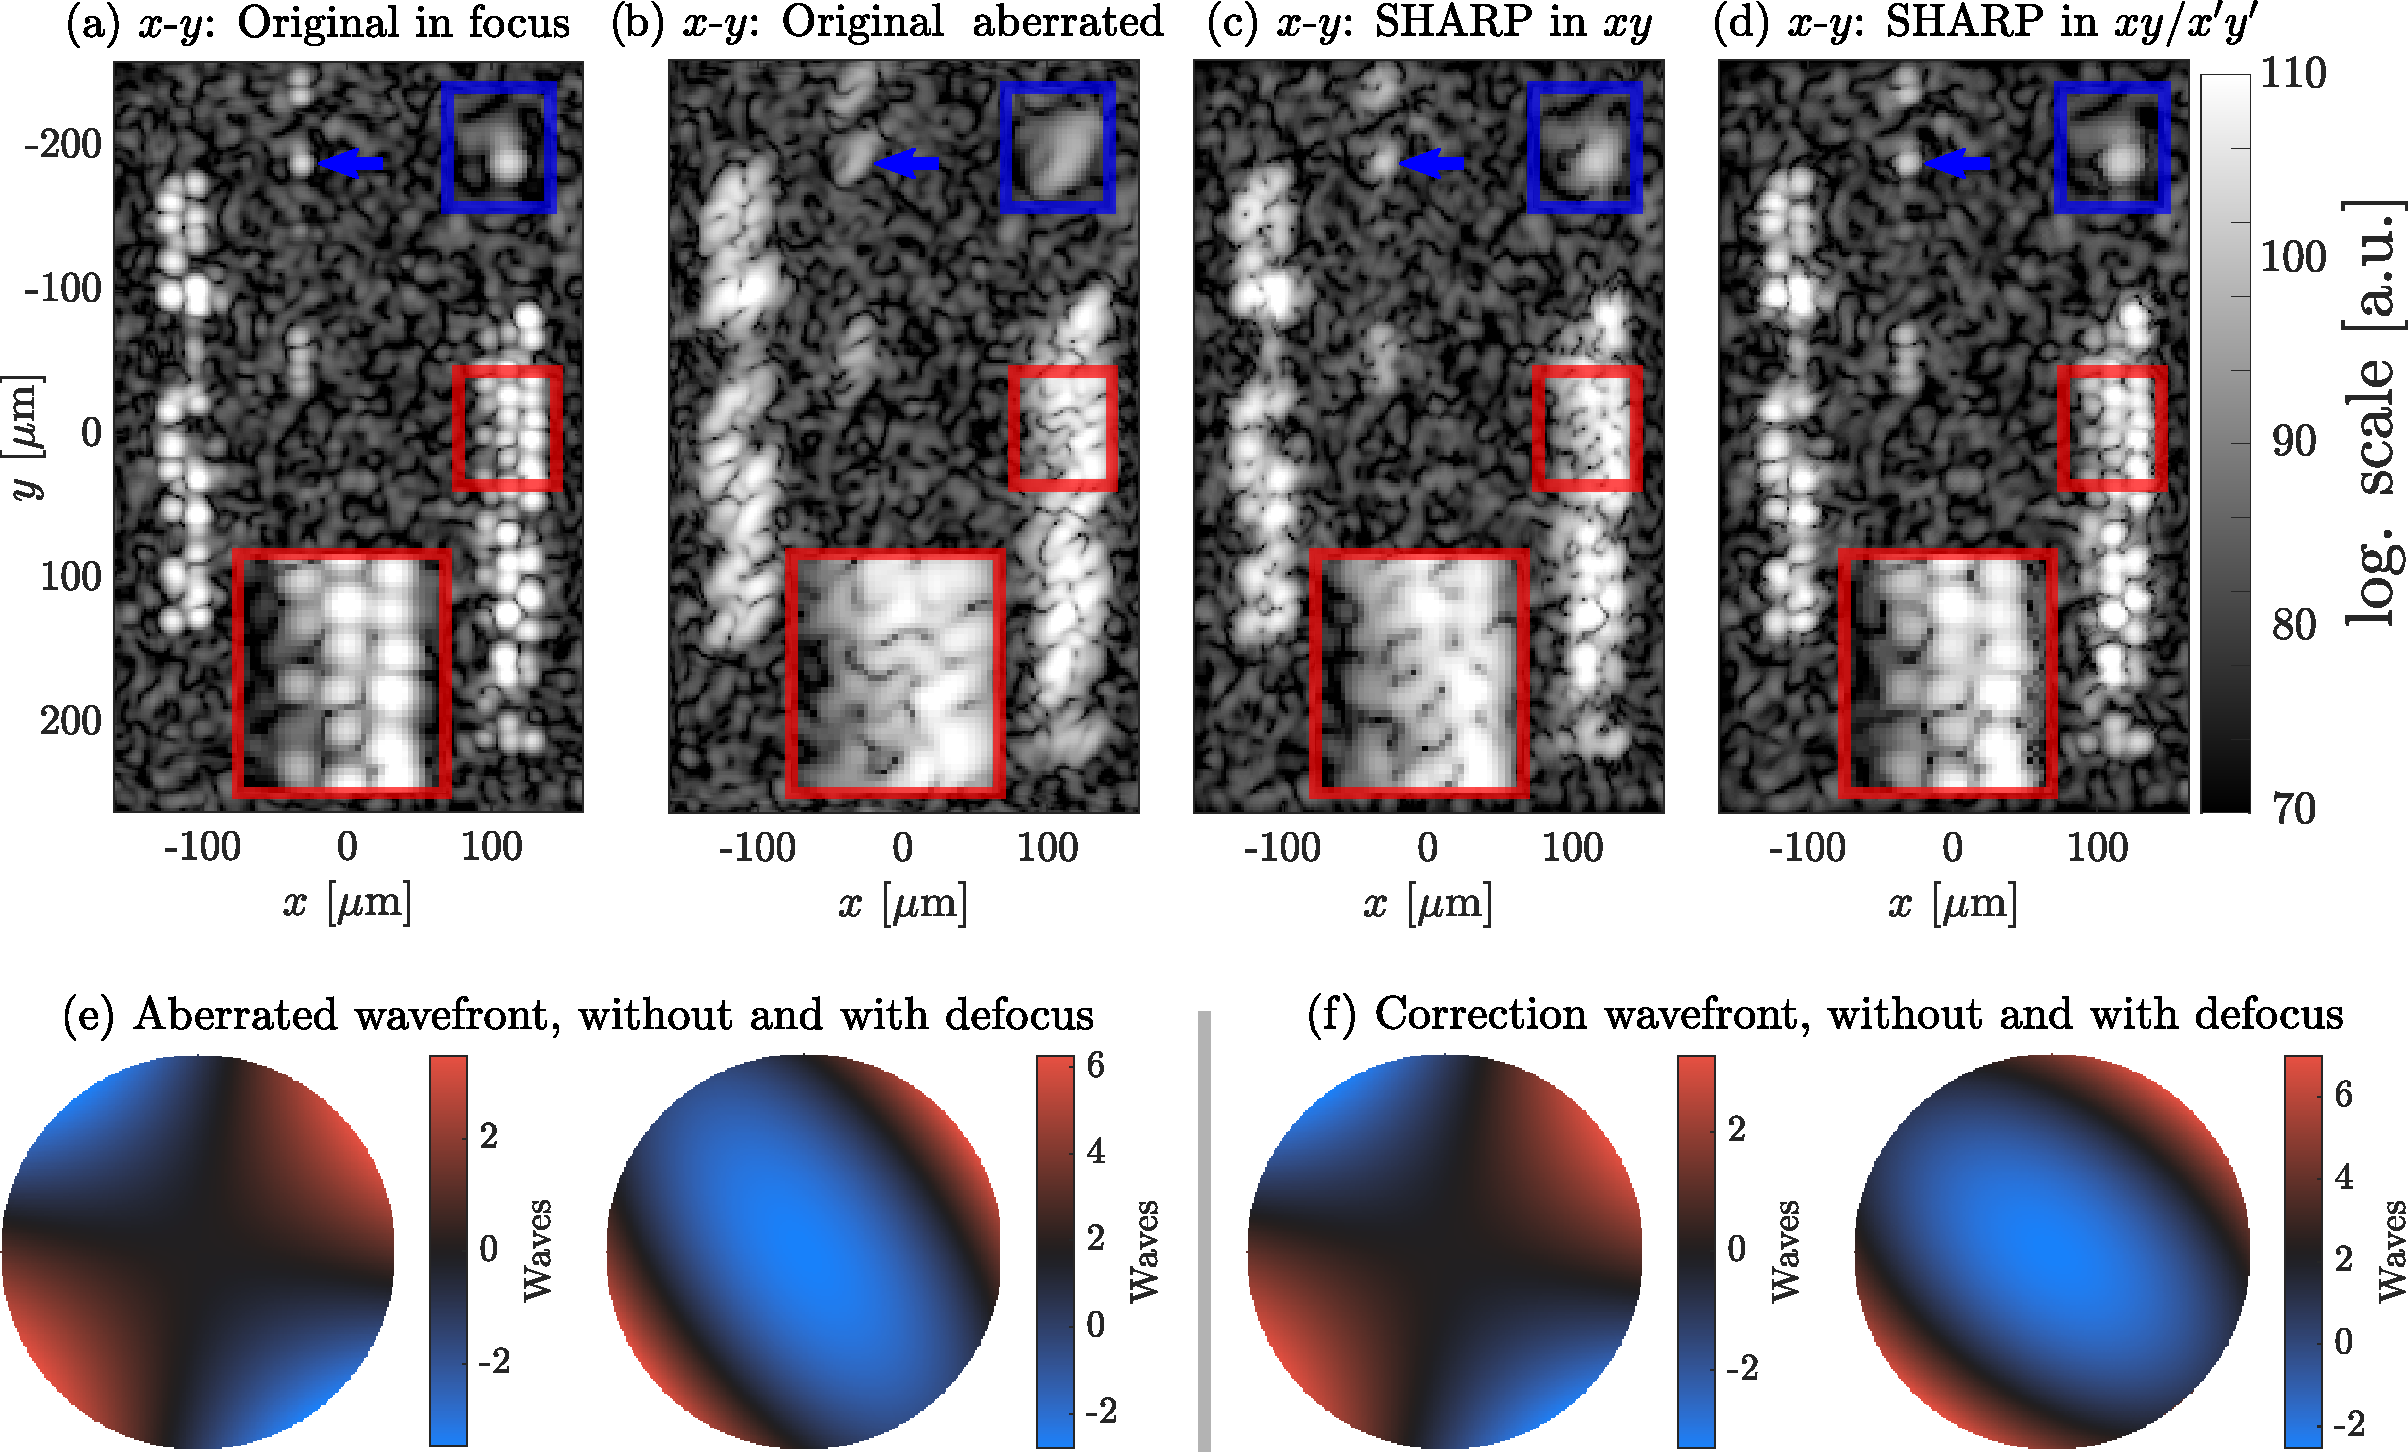
\includegraphics[width=\textwidth]{Figures/SHARP/SHARP45d_Int.pdf}
	\caption[Testing aberration correction with SHARP-$x'y'$ using a simulated OCT tomogram.]{Testing aberration correction with SHARP-$x'y'$ using a simulated OCT tomogram. \textit{En face} views of tomograms; (a) original in focus, (b) aberrated, (c) after SHARP-$xy$ and (d) subsequent SHARP-$x'y'$. Wavefront maps for the same \textit{en face} as before; (e) aberrated wavefront and (f) correction wavefront, without (left) and including defocus (right).}
	\label{fig:SHARP45d_Int}
\end{figure}

Phase noise comprising random offsets and slopes in the range $[0,\ 2\pi]$ was added to the aberrated tomogram. For describing the phase filter in 1D CAO, only Legendre polynomial $P_2$ was used. First, SHARP-$xy$ procedure was applied, obtaining partial aberration correction as visualized in the \textit{en face} plane of Fig.~\ref{fig:SHARP45d_Int}(c), followed by application of SHARP-$x'y'$ that resulted in a more noticeable image quality improvement due to aberration correction as noted in Fig.~\ref{fig:SHARP45d_Int}(d), and approaching the image quality of the original aberration-free tomogram, noted particularly when comparing the red and blue insets. Finally, the correction wavefront was computed as a superposition of the individual 1D corrections in the four axes [right panel in Fig.~\ref{fig:SHARP45d_Int}(f)] and its distribution shows that indeed correction of aberrations not oriented along the main axes $x$ and $y$ is feasible. Projection of the correction wavefront into Zernike basis yielded the weights $0.9\lambda$ for $Z_4$ and $2.2\lambda$ for $Z_5$, and using these weights to generate the correction wavefront without including defocus yields the wavefront in the left panel of Fig.~\ref{fig:SHARP45d_Int}(f).

To illustrate better the phase stabilization procedures performed along oblique axes, Figure~\ref{fig:SHARP45d_Phase} shows phase views of \textit{en face} and cross-sectional oblique planes of the original tomogram [Figs.~\ref{fig:SHARP45d_Phase}(a) and (d)], after correcting phase noise along $x'$ [Figs.~\ref{fig:SHARP45d_Phase}(b) and (e)] and along $y'$ [Figs.~\ref{fig:SHARP45d_Phase}(c) and (f)]. In the original phase images, 2D phase instability is clear. Instead, the \textit{en face} views after correcting phase noise exhibit 1D phase stability along the oblique axis. The oblique-planes images in Figs.~\ref{fig:SHARP45d_Phase}(d)-(f) showing the path marked by the white lines on the \textit{en faces}, also exhibit phase stability as expected. Interestingly, the analysis on the MPS [see Figs.~\ref{fig:SHARP45d_Phase}(g)-(i)] is yet valid for this case, only that the axis along which the MPS displays a Gaussian profile is now rotated, depending on the corrected axis.

\begin{figure}[htb!]
	\centering
	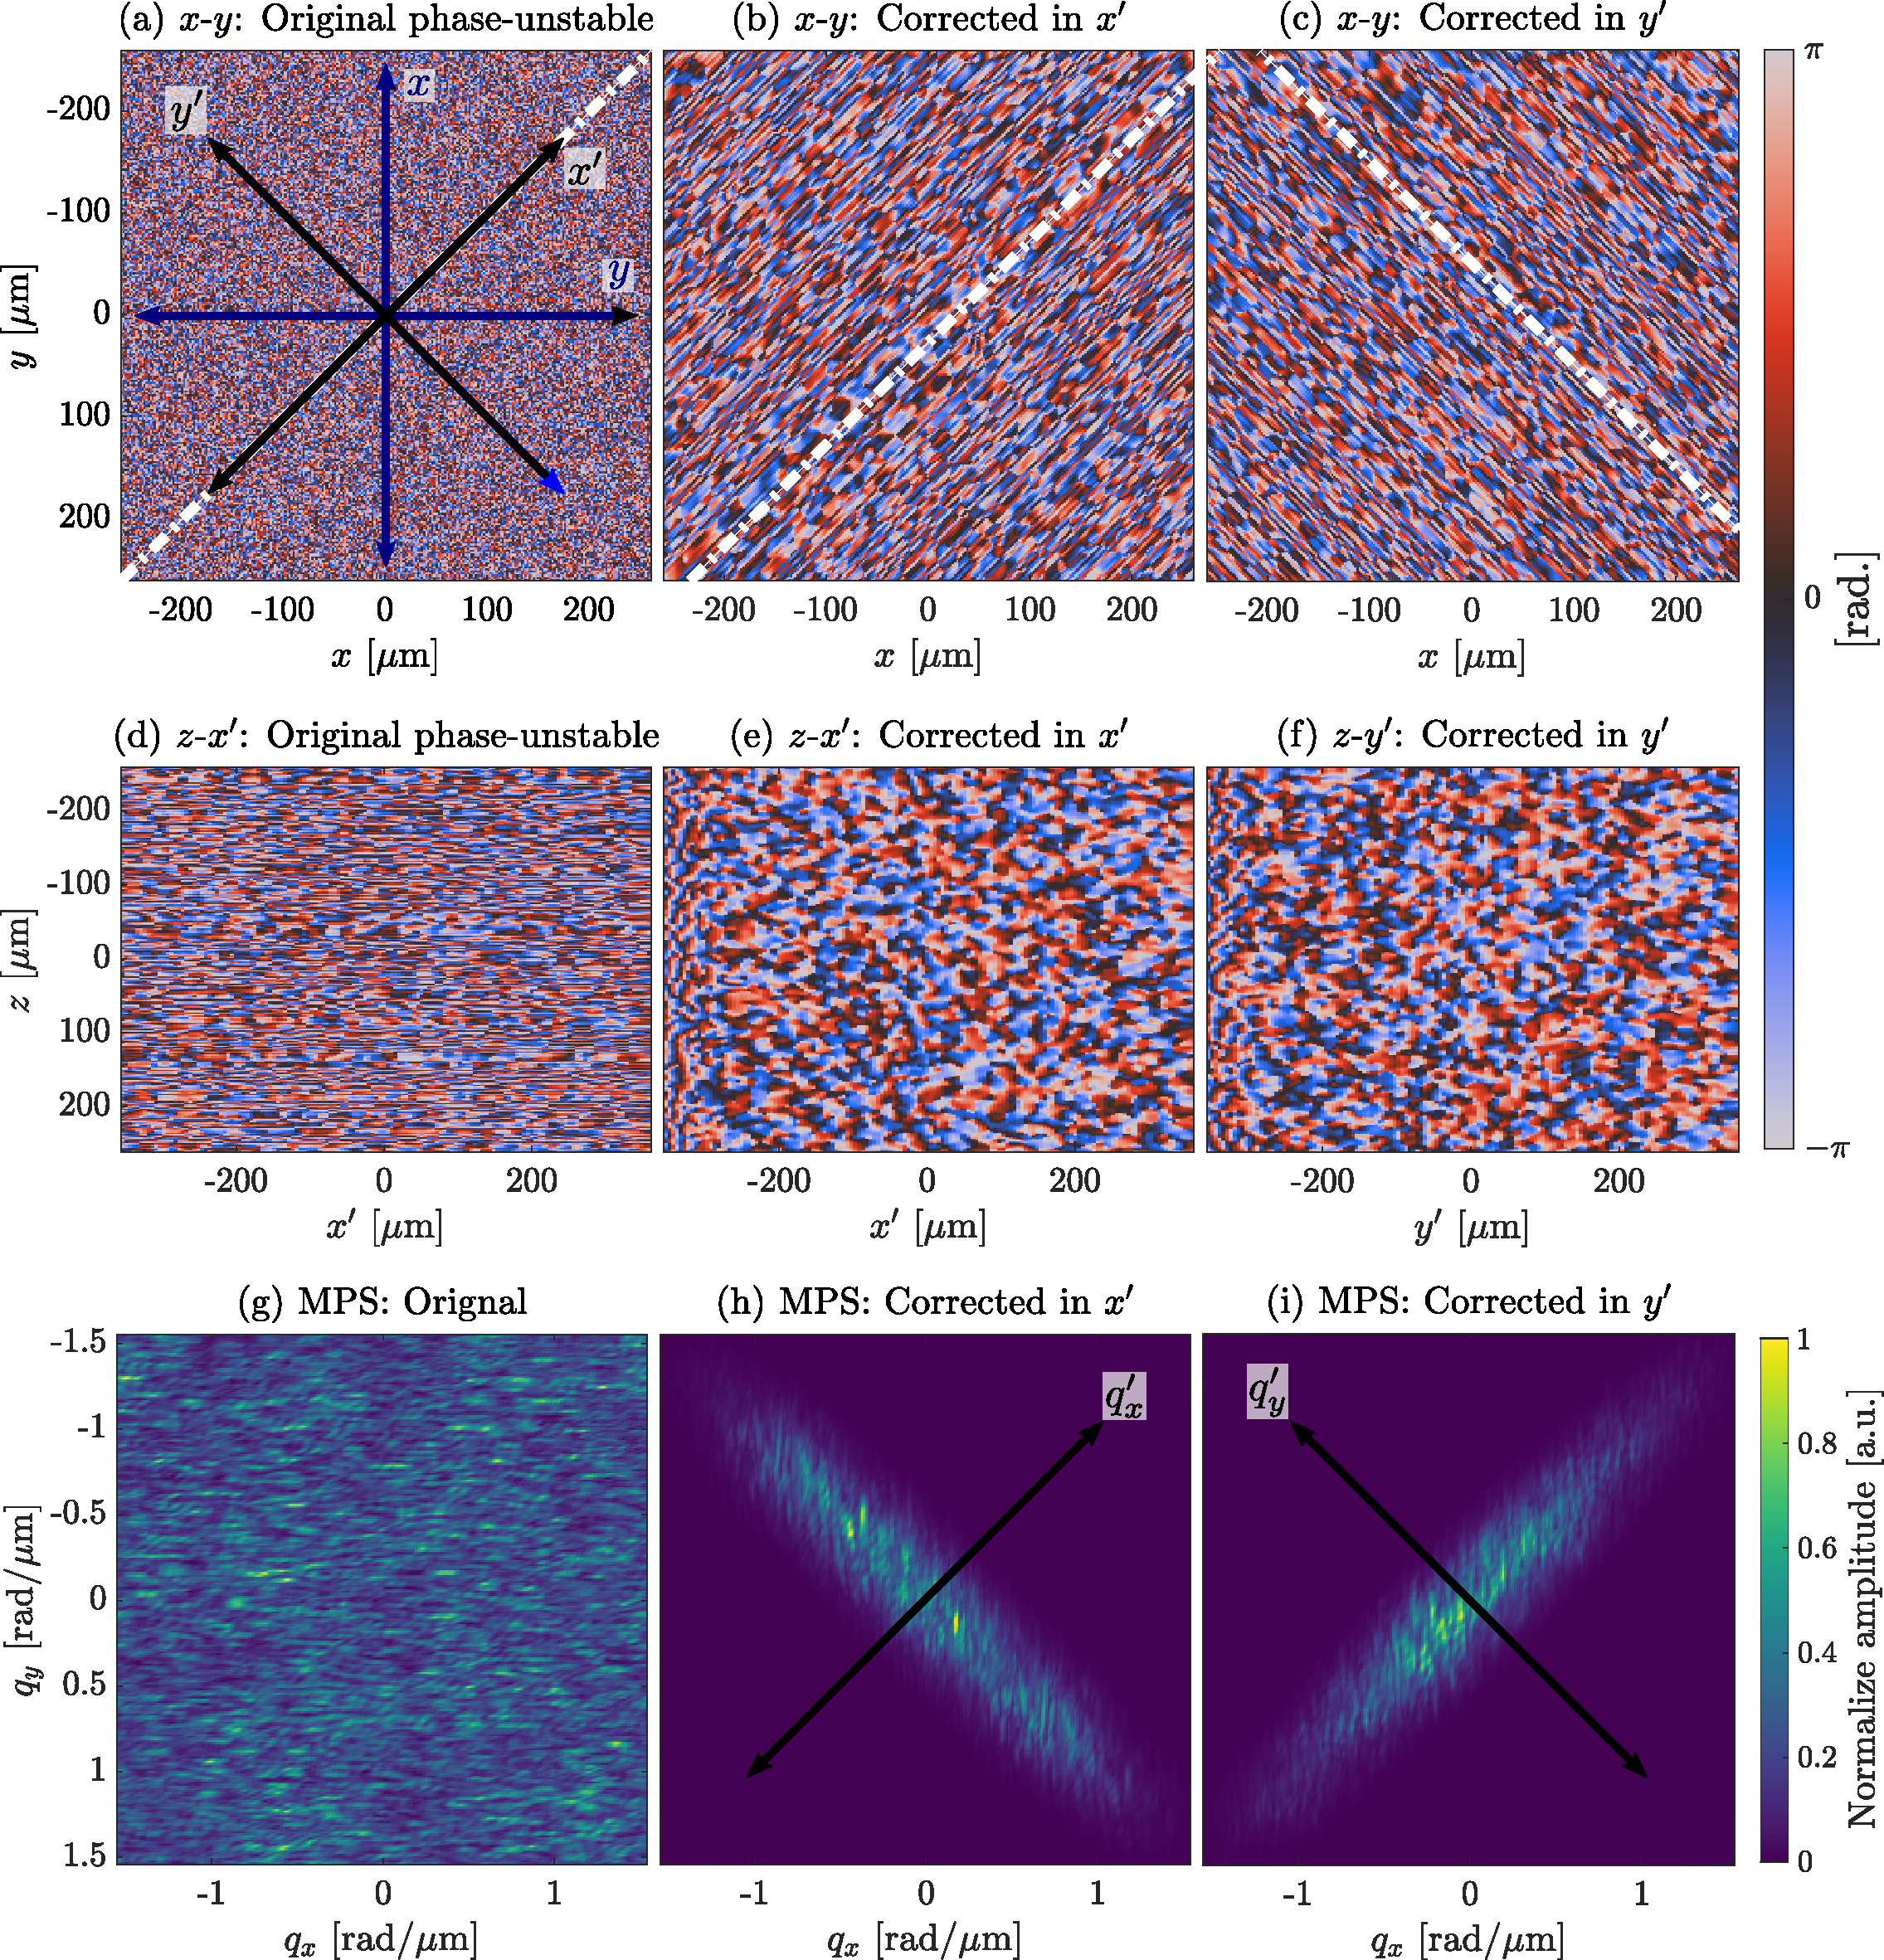
\includegraphics[width=\textwidth]{Figures/SHARP/SHARP45d_phase.pdf}
	\caption[Testing phase stabilization along oblique axes for a simulated OCT tomogram.]{Testing phase stabilization along oblique axes for a simulated OCT tomogram. \textit{En face} views of tomograms; (a) original, (b) corrected in $x'$ and (c) corrected in $y'$. Oblique cross-sections $z$-$x'$; (d) original and (e) corrected in $x'$. (f) Oblique cross-sections $z$-$y'$ corrected in $y'$. MPS of tomograms; (g) original, (h) corrected in $x'$ and (i) corrected in $y'$. Note that axes in the MPS maps are $q_x$, $q_y$ and not $q_{x'}$, $q_{y'}$.}
	\label{fig:SHARP45d_Phase}
\end{figure}

% When dofocus is the dominant aberration, independent results from SHARP-$xy$ and SHARP-$x'y'$ should be very similar given that the quadratic phase used to represent defocus can be fully described using either the main axes or the rotated ones. Therefore, a readily verification of SHARP-$x'y'$ in an experimental dataset could be performed using the OoF tomogram of the \textit{cucumis sativus} sample used in Section~\ref{sec:Test}, to complement the previous verification with the simulated dataset. Figure~\ref{fig:SHARP_EnfacesComp} shows an \textit{en face} plane of the original OoF tomogram in Fig.~\ref{fig:SHARP_EnfacesComp}(a), after SHARP-$xy$ in Fig.~\ref{fig:SHARP_EnfacesComp}(b) and after SHARP-$x'y'$ in Fig.~\ref{fig:SHARP_EnfacesComp}(d). Defocus of original image was successfully corrected with both procedures, showing its equivalence for defocus correction.

% Also, a experimental validion of  windows-based SHARP-$xy$ was also applied and show in Fig.~\ref{fig:SHARP_EnfacesComp}(c), obtaining that 

% \begin{figure}[htb!]
% 	\centering
% 	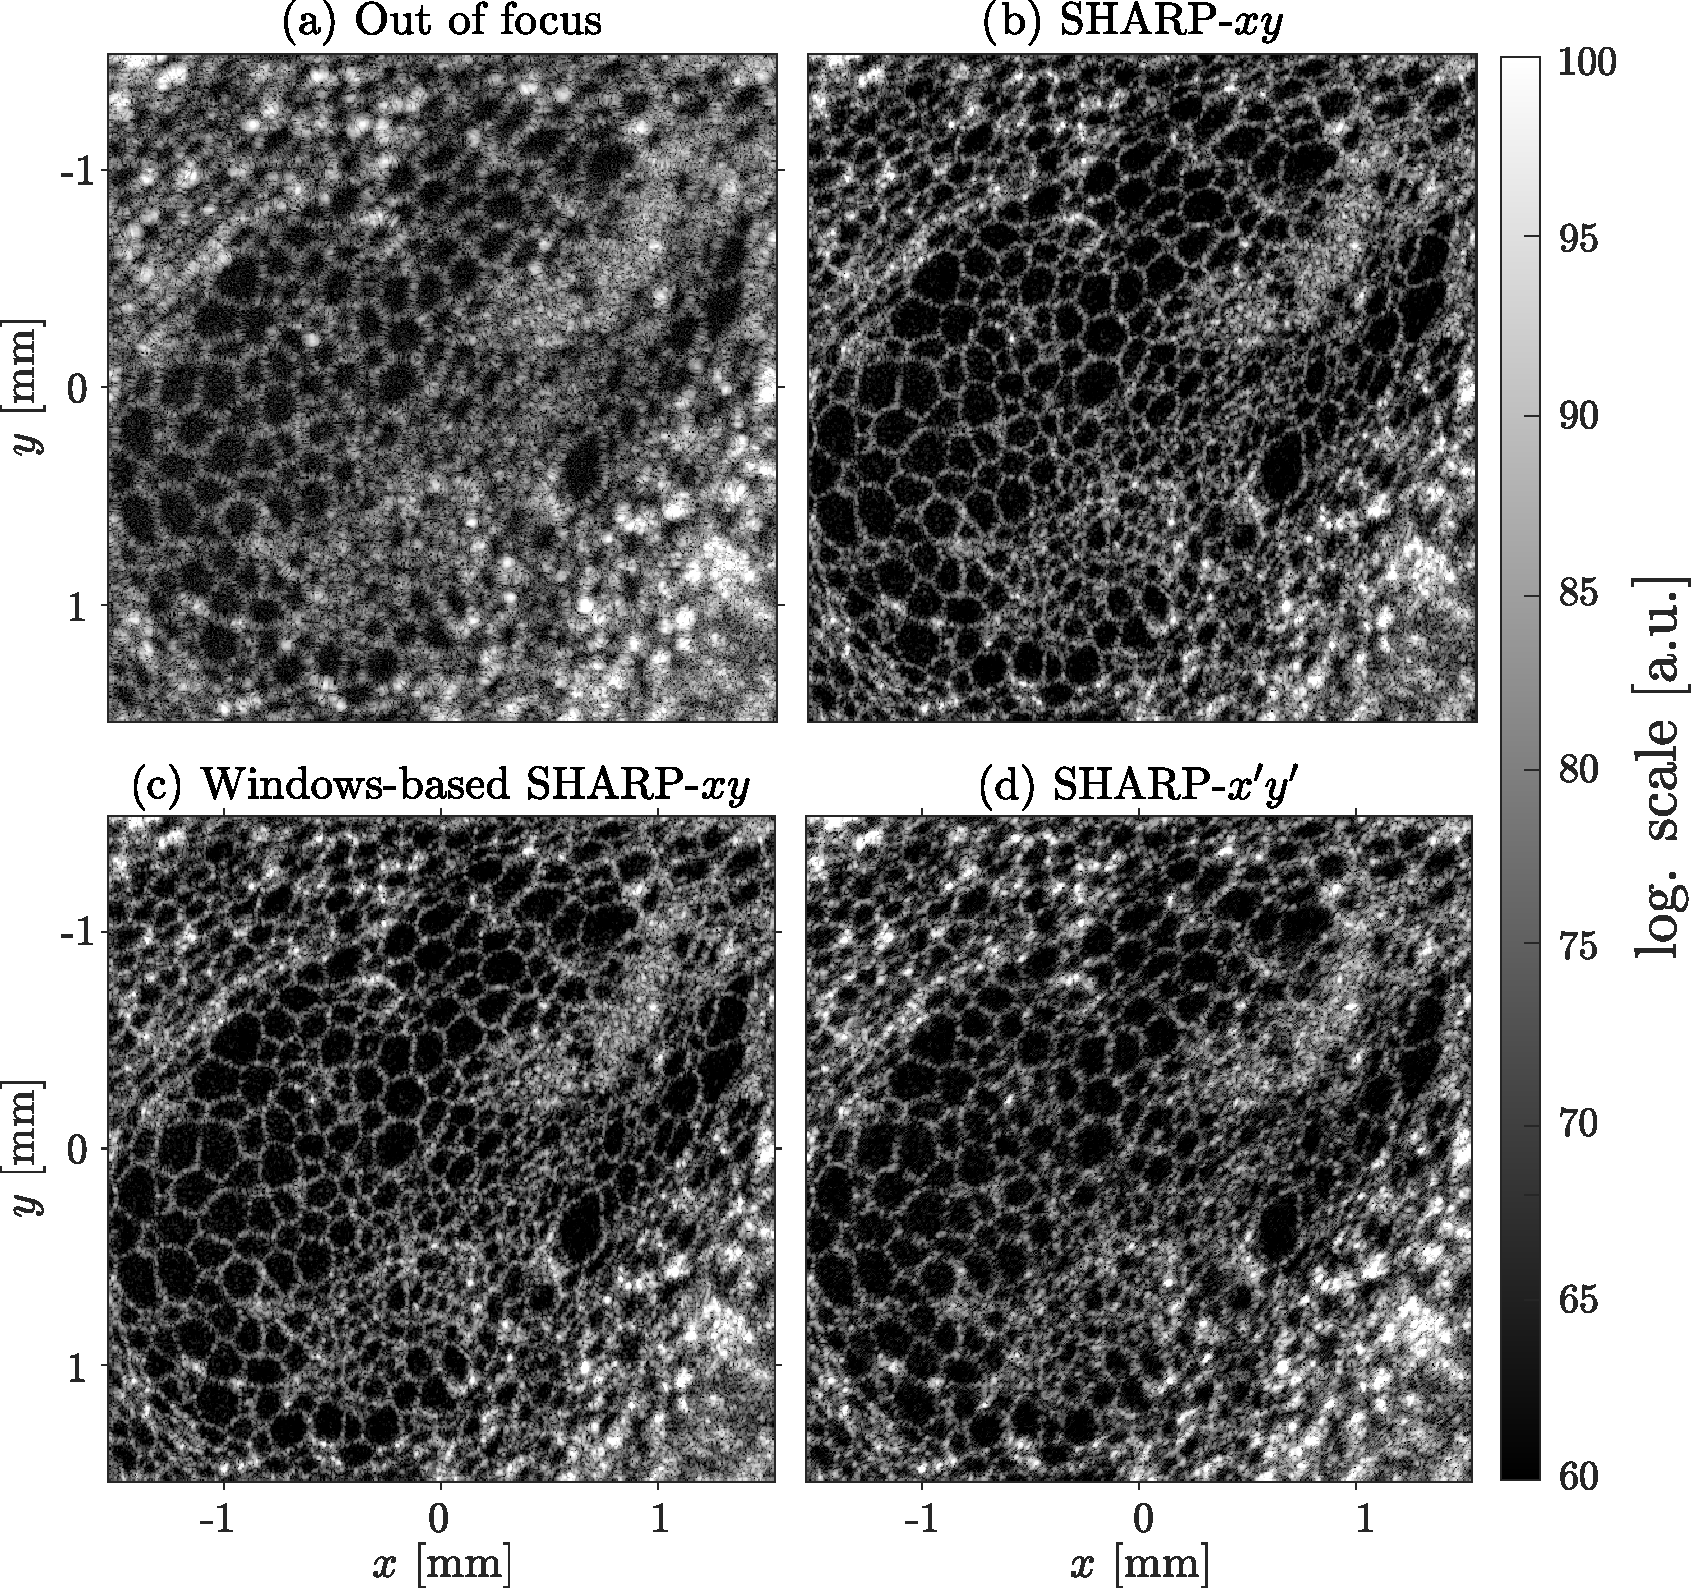
\includegraphics[width=.8\textwidth]{Figures/SHARP/SHARP_ExtensionsEnfaces.pdf}
% 	\caption[Testing phase stabilization along oblique axes for a simulated OCT tomogram.]{Testing phase stabilization along oblique axes for a simulated OCT tomogram. \text{En face} views of tomograms; (a) original in focus, (b) aberrated, (c) after SHARP-$xy$ and (d) SHARP-$x'y'$.}
% 	\label{fig:SHARP_EnfacesComp}
% \end{figure}

\FloatBarrier

\subsection{Computational aberration correction in polarization-sensitive OCT}

The operation of CAC techniques so far has been described for intensity images used for structural contrast, however, in functional extensions of OCT the effects of aberrations in the acquired complex signal is also transferred through the post-processing methods used for calculating additional useful information of the sample, such is the case of polarization-sensitive (PS-)OCT, which is used for the measurement of polarimetric properties of tissue~\cite{deBoer1997_Twodimensional, deBoer2017_Polarization}. PS-OCT has great clinical interest due to its sensitivity to fibrillar tissue and its organization, and is used in intravascular OCT~\cite{Villiger2018_Coronary}, retinal imaging~\cite{Elmaanaoui2011_Birefringence, Cense2009_Retinal}, anterior segment~\cite{Li2020_Vectorial}, among others applications. Adaptive optics (AO) has been integrated into PS-OCT systems for aberration-free retinal imaging with improved effective lateral resolution~\cite{Cense2009_Retinal}, however, it is known that AO does not extend the depth of field, whereas numerical alternative like ISAM or CAO are capable of extending the depth of field by correcting for the depth-dependent defocus. The phase stability requirement has hindered adoption of CAC technique in many systems oriented to PS-OCT that may not satisfy the phase stability requirement. Apart from the work of Davis \textit{et. al.} where they developed a vectorial description of ISAM for polarization-sensitive imaging~\cite{Davis2007_Nonparaxial, Davis2007_Polarimetric}, CAC techniques have not been demonstrated in PS-OCT, and thus it is unclear whether the processing performed in such techniques affects negatively the PS-OCT processing.

Given that SHARP can operate with phase-unstable systems, its operation can be extended to PS-OCT systems which often do not satisfy the phase stability requirement. In this section, a procedure to properly apply SHARP in PS-OCT taking into consideration the particularities of Stokes tomograms processing is presented. Because the theory and models used in PS-OCT are rather extensive and out of scope of this work, only the sufficient information required to understand the operation of SHARP in PS-OCT is provided here, and detailed information if required by the reader can be explored in addition bibliography~\cite{deBoer2017_Polarization, Villiger2013_Spectral}.

\subsubsection{Overview of Stokes processing}

In PS-OCT processing, briefly summarized in Figure~\ref{fig:PSOCTProc}, the polarimetric properties of the backscattered light by the sample are retrieved from a collection of several polarization-diverse measurements. More specifically, the sample is illuminated using two polarization states $p=\{p_1, p_2\}$ orthogonal in the Poincar\'e sphere and the backscattered signal is measured by a polarization-diverse receiver with two orthogonal polarization channels $c=\{c_1, c_2\}$, for a total of four tomographic complex measurements $S_{p,c}(x,y,z)$. In standard Stokes processing for PS-OCT, these four complex measurements forming two Jones vectors are converted into two Jones-Stokes vectors $\mathbf{\mathbb{S}} = [I, Q, U, V]^T$ composed of the four Stokes parameters from which polarimetric properties of the sample are calculated~\cite{deBoer2017_Polarization}, being $I$ the total intensity and $Q$, $U$ and $V$ quantities related to the degree of linear, oblique and circular polarization, when properly normalized. Polarimetric properties retrieved in Stokes processing are degree of polarization (DOP) and birefringence comprising phase retardation or retardance $\Delta n$ and optic-axis orientation $\psi$. 

%Polarization-diverse detection consist in placing a polarization-dependent beam splitter in the output of the interferometer to split the light into two orthogonal polarization states, typically horizontal and vertical states, and each one is detected by an independent detector. To generate the two illumination polarization states, advanced active elements are used like electro-optic modulator (OEM) to dynamically interchange the polarization state between pair of A-lines during the measurement, a method known as inter-A-line modulation, or passive elements like polarization delay units (PDU) that separates the light into two polarization states which are then delayed by a constant optical path length resulting in the two polarization states being depth-encoded in the acquired tomogram.

Because of the coherent nature of OCT signal, the Jones-Stokes vectors are affected by speckle which appears as strong noise in the subsequent calculation of polarimetric properties. For this reason, each Jones-Stokes parameter is spatially averaged, typically using a Gaussian kernel, to produce incoherent Stokes parameters $\mathbf{\bar{\mathbb{S}}}~=~[\bar{I}, \bar{Q}, \bar{U}, \bar{V}]^T$ with reduced speckle resulting in polarimetric properties with reduced noise. However, a resolution loss is associated to this spatial average, which in combination to aberrations have imposed a relatively coarse lateral resolution in PS-OCT imaging~\cite{Cense2009_Retinal}, making difficult to obtain highly-localized measurement of polarimetric properties of tissue which may be of great interest~\cite{Cense2009_Retinal, Li2020_Vectorial}.

\begin{figure}[htb!]
	\centering
	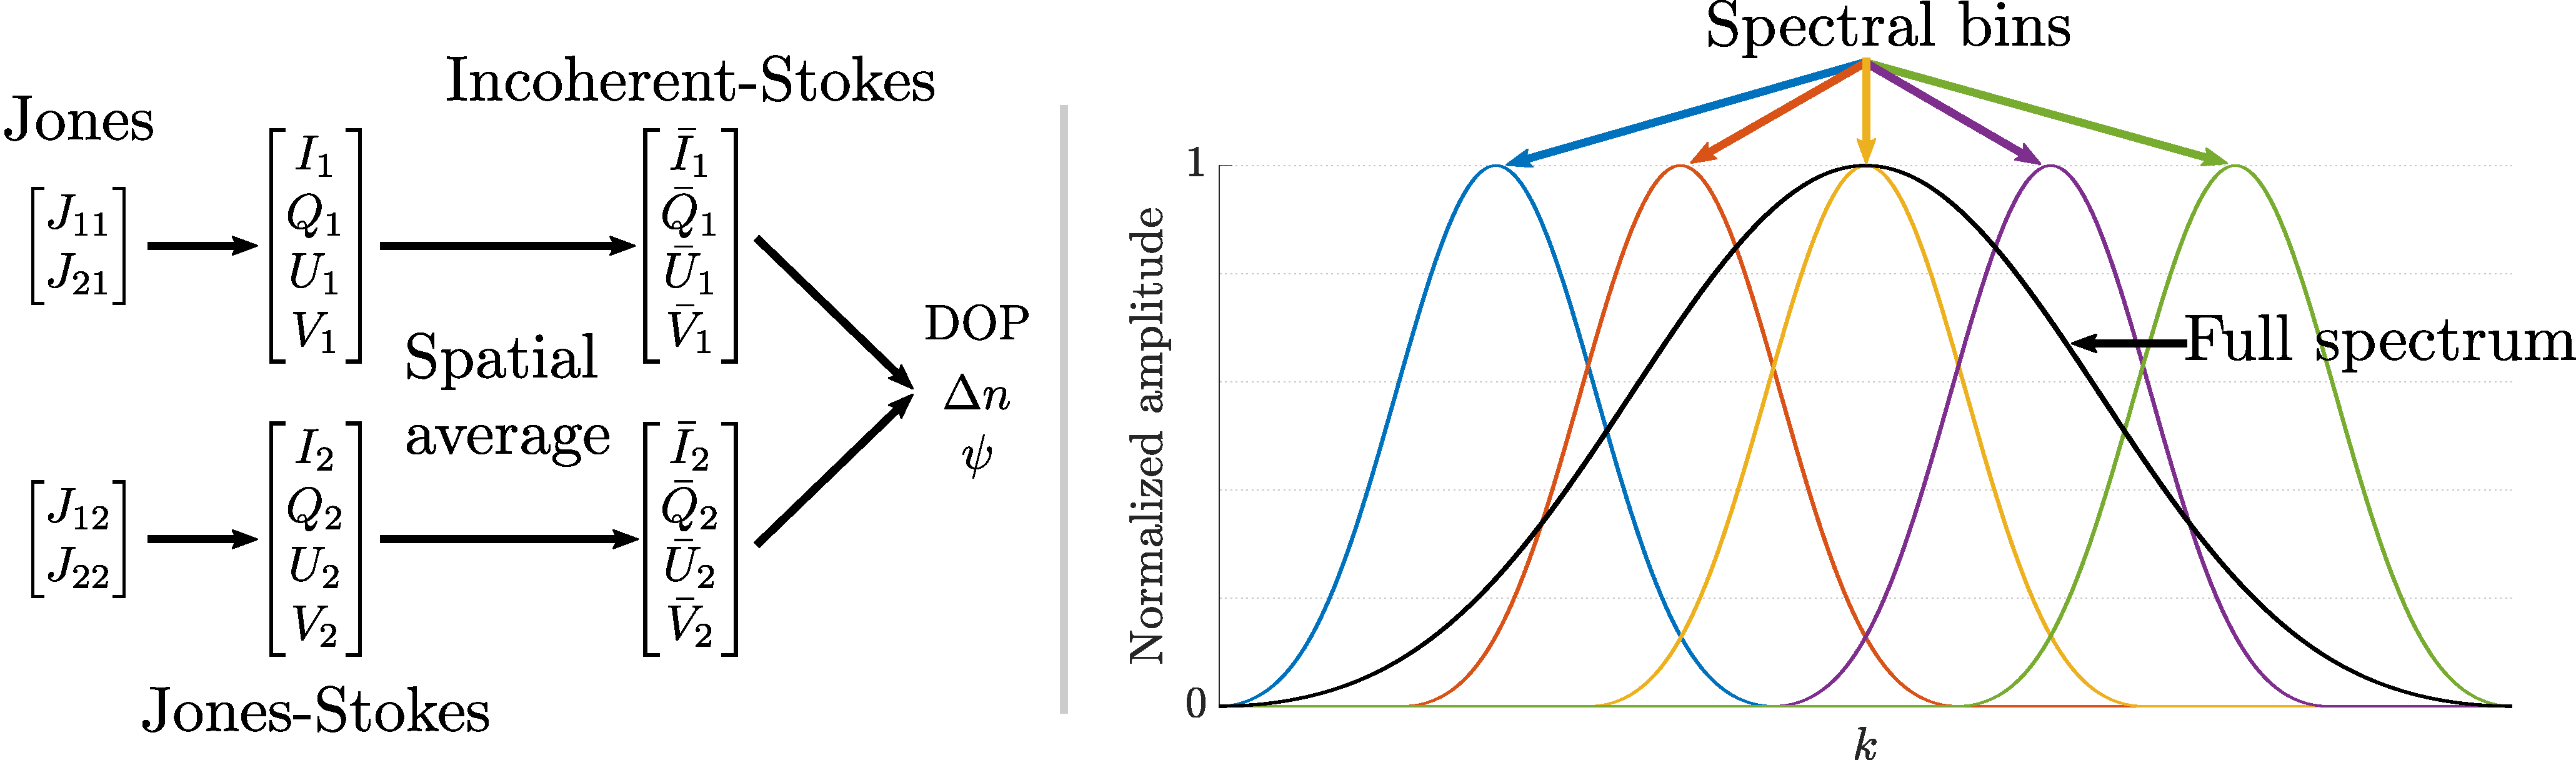
\includegraphics[width=\textwidth]{Figures/SHARP/PSOCT-Processing.pdf}
	\caption[Overwiew of Stokes processing for PS-OCT and spectral binning.]{Overwiew of Stokes proccesing for PS-OCT and spectral binning.}
	\label{fig:PSOCTProc}
\end{figure}

In certain PS-OCT systems, fiber-based components induce wavelength-dependent changes on the polarization state of light that prevent to obtain reliable information from the acquired signals $S_{p,c}(x,y,z)$ directly~\cite{deBoer2017_Polarization}. To overcome this, spectral binning processing has been proposed~\cite{Villiger2013_Spectral}, in which the acquired spectral signals $S_{p,c}(x,y;k)$ in $k$-space are splitted into several bins covering smaller portions of the bandwidth, as depicted in Fig.~\ref{fig:PSOCTProc}, such that wavelength-dependent effect of the system is made more constant within each spectral bin since they have a narrower bandwidth than the original spectrum. Then, PS-OCT processing is performed independently for each reduced-bandwidth tomogram, with additional steps based on vectorial analysis to align the estimated polarimetric properties into a single estimation comprising the information of the entire original spectrum~\cite{Villiger2013_Spectral}. There is an additional resolution loss in spectral binning processing, but this time in the axial direction only, because the bandwidth of each spectral bin is narrower than the original spectrum, resulting in a coarser axial resolution.

\subsubsection{Polarization-sensitive SHARP}

Given that aberration correction operates on the complex field, SHARP must be applied on the four complex tomograms $S_{p,c}$ prior to conversion to Stokes parameters which are intensity values. Particularities of the process are following explained, but first, it should be clarified that the goal here is to correct non-polarizing aberrations, which are different to polarization aberrations that include changes in the polarization state of light associated with ray paths through optical systems~\cite{Chipman1989_Polarization}.

The determination of the optimal weights for CAO from individual spectral bins tends to be ineffective since each spectral bin has a reduced axial resolution and different amount of signal-to-noise ratio. Therefore, the tomogram with the full spectral bandwidth of the system is employed to determine the optimal weights via optimization rather than finding the optimal weights for each spectral bin independently. The optimization procedure is performed only for a single polarization state $p$ and the image sharpness metric is calculated from the total intensity given by $|S_{p,c1}|^2 + |S_{p,c2}|^2$, assuming that aberrations are polarization-independent thus they are the same for both polarization states. Strictly speaking, polarizing media may induce undesired changes in wavefront that depend on the polarization state of light, but magnitude of these changes have generally a small contribution compared to wavefront aberrations, even more with the magnitude of polarizing effects of tissue.

Phase offsets and slopes required for phase stabilization are determined also in the full-bandwidth tomogram but for the two polarization states $p$ independently because phase noise is not necessarily the same. After determining phase noise correction (offsets and slopes) and the optimal weights for aberration correction using the full-bandwidth tomograms, these parameters are then applied to all spectral bins and input polarization states. To summarize, operation of SHARP in PS-OCT consists in determining the parameters for phase noise and aberration correction in the full-bandwidth tomograms and then using those to correct each spectral bin independently. This is possible since the filter applied in CAO is $k$-independent and since phase noise correction operates on each A-line globally and therefore it does not change across spectral bins. Aberration-corrected complex tomograms  $\tilde{S}_{p,c}$ for each spectral bin are then transformed into Stokes vectors followed by the subsequent steps in PS-OCT processing. The positive effect of CAO applied to the complex tomograms is translated into the Stokes parameters and ultimately into the polarimetric properties.

\section{Complex noise reduction: CTNode}\label{sec:CTNode}

High sensitivity of typically $\sim$100~dB is provided by OCT system, meaning that backscattered light as weak as $10^{-10}$ times the reference mirror reflection can still be detected~\cite{Choma2003_Sensitivity, deBoer2003_Improved}. Further improvements are possible with post-processing, and most used approach consists in averaging multiple frames to reduce noise, taking advantage of the high imaging speed provided by FDOCT that enables to acquire multiple repeated frames~\cite{Baumann2019_Signal, Szkulmowski2013_Averaging}. Averaging can be either incoherent, i.e. using the intensity signal, or coherent, i.e. using the complex signal, but it has been found that coherent averaging is more efficient in improving the SNR in phase stable data~\cite{Baumann2019_Signal}. Although frame averaging has been effective to increase SNR of OCT images for an improved visualization and diagnosis~\cite{Sakamoto2008_SpectralDomain}, it demands the acquisition of multiple frames which is unpractical in certain scenarios, specially in volumetric imaging given the large amount of data, the significant increase in acquisition time and the susceptibility to be negatively affected by motion artifacts. 

Analyzing and addressing noise in complex signal is advantageous for phase-dependent post-processing techniques~\cite{Uribe-Patarroyo2020_Noise}. In particular, in CAC there is an explicit interest in improving SNR because aberrations produce a significant reduction of signal collection, and as a consequence acquired images have a reduced dynamic range that is not expanded by aberration correction. The optimum amplitude filter integrated in SHARP is a straightforward tool to address noise and although its performance could be improved by means of oversampling, its effectiveness is limited specially when sampling approaches Nyquist.

In this section, a statistical approach for noise reduction is proposed as an alternative to current strategies, in which the 2D or volumetric information of the tomogram is exploited to reduce noise with no need of frames repetitions. The framework of this proposal is based on the previously developed technique \textbf{T}omographic \textbf{NO}n-local means \textbf{de}speckling (TNode) that suppresses speckle on the intensity while preserving resolution~\cite{Cuartas-Velez2018_Volumetric}, except that here the aim is to denoise the complex signal thus the new proposal is called \textbf{C}oherent \textbf{T}omographic \textbf{NO}n-local means \textbf{de}noising (CTNode). A description of CTNode is provided below.

\subsection{Non-local means}

Non-local means has been used widely in image processing in several fields~\cite{Deledalle2015_NLSAR,Lu2012_Nonlocal,Yu2016_Probabilitybased,Coupe2008_Optimized} as it outperforms traditional averaging in resolution preservation. The core idea behind non-local means is to perform a spatial average using an adaptive kernel defined explicit for each pixel of the image using the information of neighboring pixels~\cite{Cuartas-Velez2018_Volumetric}. To define the weights of the kernel used to filter a target pixel, a statistical metric is used to determine how similar are each neighboring pixel to the target pixel. Defining the acquired noisy tomogram as $S_N(\bm{r})$ with $\bm{r}$ being a 3D vector representing the three coordinates $\bm{r}=(x,y,z)$, the weighted estimation $\hat{S}(\bm{r})$ of the noiseles signal $S(\bm{r})$ is computed as
\begin{equation}\label{eq:NLM}
    \hat{S}(\mathbf{r}) = \frac{\sum_{\bm{r}'\in \bm{\nu}} w(\bm{r}, \bm{r}') S_N(\bm{r}')}{\sum_{\bm{r}'\in \bm{\nu}} w(\bm{r}, \bm{r}')}
\end{equation}
where $w(\bm{r}, \bm{r}')$ are the weights of target pixel $\bm{r}$ with respect to all neighbor pixels $\bm{r}'$ inside a search windows $\bm{\nu}$. The search windows $\bm{\nu}$ is a collection of pixels centered at $\bm{r}$ with sizes $(\nu_x, \nu_y, \nu_z)$ for a total size of $V=(2\nu_x+1)\times(2\nu_y+1)\times(2\nu_z+1)$ that defines the spatial extension of the filtering kernel. In order words, the search window controls how many pixels are included in the weighted average of target pixel. The following step is to find a proper definition of $w(\bm{r}, \bm{r}')$ based on statistical properties of noise in order to produce an appropriate filtering.

\subsection{Derivation of weights for noise reduction}

Noise in FDOCT is originated in the acquisition of the spectral fringes under an additive model, allowing to express the measured noisy signal in $k$-space as $s_n(x,y,k) = s(x,y,k) + n(x,y,k)$ where $s(x,y,k)$ is the true noiseless signal and $n(x,y,z)$ is the randomly distributed noise. After Fourier transform of the spectral fringes used to compute the depth-dependent signal $S_N(x,y,k)$, noise still follows an additive model since
\begin{align}
    \text{FT}_k\{s_n(x,y,k)\} &= \text{FT}_k\{s(x,y,k)\} + \text{FT}_k\{n(x,y,k)\} \nonumber\\
    S_N(\mathbf{r}) &= S(\mathbf{r}) + N(\mathbf{r}),
\end{align}
where $S(\mathbf{r})$ is the true noiseless depth-dependent signal and $N(\mathbf{r})$ the additive noise, setting $\mathbf{r} = (x,y,z)$ for simplicity as before. The task is therefore to cancel out the contribution of noise. It has been shown that noise in OCT follows a zero-mean complex Gaussian distribution with equal standard deviation $\sigma_N$ on both the real and imaginary parts~\cite{Makita2016_Noiseimmune, Uribe-Patarroyo2020_Noise}. Analyzing only the real part of the signal $R_N = \text{Re}\{S_N\}$ by now, the probability of measuring a realization $R_N$ given a true value $R = \text{Re}\{S\}$ and the standard deviation $\sigma_N$ of noise is~\cite{Deledalle2012_How}
\begin{equation}\label{eq:GaussianProb}
    \mathcal{P}(R_N|R, \sigma_N) = \frac{1}{\sqrt{2\pi}\sigma_N} \exp\left\{-\frac{(R_N-R) ^ 2} {2\sigma_N^2}\right\}
\end{equation}
and similarly for the imaginary part $I_N = \text{Im}\{S_N\}$.

To determine the similarity between a pair of values $R_N(\bm{r})$ and $R_N(\bm{r}')$, a similarity criterion is defined using the likelihood-ratio test (LRT),
\begin{equation}
    \mathcal{L}\{R_N(\bm{r}), R(\bm{r})\} = \frac{\mathcal{P}[R_N(\bm{r})|R(\bm{r},\bm{r}'), \sigma_N] \mathcal{P}[R_N(\bm{r}')|R(\bm{r},\bm{r}'), \sigma_N]} {\mathcal{P}[R_N(\bm{r})|R(\bm{r}), \sigma_N] \mathcal{P}[R_N(\bm{r}')|R(\bm{r}'), \sigma_N]}
\end{equation}
which evaluates the probability that the underlying noiseless parameters $R(\bm{r})$ and $R(\bm{r}')$ are different between them or equal to a common parameter $R(\bm{r}, \bm{r}')$. The standard deviation of noise is assumed equal in all probabilities given that $\sigma_N$ tends to be constant over the entire tomogram. More specifically, the numerator of the LRT is the probability of the two values $R_N(\bm{r})$ and $R_N(\bm{r}')$ being different realizations of the same distribution, in which case the similarly is high and the numerator tends to one, while the denominator is the probability of the two values $R_N(\bm{r})$ and $R_N(\bm{r}')$ being realizations of different distributions, in which case the similarity is small and the denominator tends to a large value. In consequence, the LRT tends to one when the two pixels being compared are likely similar and to zero when they are dissimilar.

In practice, the underlying parameters are in general unknown and the LRT cannot be computed directly, therefore it is replaced by the generalized likelihood ratio (GLR) $\mathcal{L}_G$~\cite{Cuartas-Velez2018_Volumetric} where the parameters are changed by their maximum likelihood estimates~\cite{Deledalle2012_How}, enabling to obtain a closed-form expression given by
\begin{equation}\label{eq:GLR}
    \mathcal{L}_G\left\{R_N(\bm{r}), R_N(\bm{r}')\right\} = \exp\left\{-\frac{[R_N(\bm{r}) - R_N(\bm{r}')]^2} {4\sigma_N^2}\right\}
\end{equation}
for the case of the Gaussian distribution of Eq.~\eqref{eq:GaussianProb}. The GLR in Eq,\eqref{eq:GLR} was derived using the real part of the signal, but the expression for the imaginary part is equivalent. The probability of the real and imaginary parts must be compounded in order to avoid corruptions in the phase due to dissimilar filtering. This compounding imposes the condition that two pixels are similar only when the real \textit{and} imaginary parts are similar. Hence, the GLR for the complex signal $\mathcal{L}_C$ is
\begin{align}\label{eq:GLR_total}
    \mathcal{L}_C\left\{S_N(\bm{r}), S_N(\bm{r}')\right\} &= \exp\left\{-\frac{[R_N(\bm{r}) - R_N(\bm{r}')]^2} {4\sigma_N^2}\right\} \exp\left\{-\frac{[I_N(\bm{r}) - I_N(\bm{r}')]^2} {4\sigma_N^2}\right\} \nonumber\\
    &=  \exp\left\{-\frac{[R_N(\bm{r}) - R_N(\bm{r}')]^2 + [I_N(\bm{r}) - I_N(\bm{r}')]^2} {4\sigma_N^2}\right\} \nonumber\\
    &= \exp\left\{-\frac{|S_N(\bm{r}) - S_N(\bm{r}')|^2} {4\sigma_N^2}\right\},
\end{align}
where the property of complex numbers $|\mathcal{Z}|^2 = \text{Re}\left\{\mathcal{Z}\right\}^2 + \text{Im}\left\{\mathcal{Z}\right\}^2$ was employed. $\mathcal{L}_C$ depends only in the two observed values $S_N(\bm{r})$, $S_N(\bm{r}')$ and the standard variation of noise that can be estimated experimentally. 

The GLR is a point-wise estimation but comparing patches of pixels around the two pixels of interest could yield a more robust estimation. Similarity between patches $\mathcal{L}_{P}$ is calculated by computing the point-wise similarity between corresponding pixels of the patches and then compounding the logarithmic probabilities as
\begin{equation}
    \mathcal{L}_{P}\left\{S_N(\bm{r}), S(\bm{r}')\right\} = \sum_{\bm{\tau}\in\bm{p}}\log\{\mathcal{L}_C[S_N(\bm{r}+\bm{\tau}), S_N(\bm{r}'+\bm{\tau})]\}
\end{equation}
where $\bm{p}$ is a collection of 3D shifts such that $\bm{r}+\bm{\tau}$ and $\bm{r}'+\bm{\tau}$ span the pixels in the patches around $\bm{r}$ and $\bm{r'}$, respectively, which are called similarity windows having sizes $(p_x, p_y, p_z)$ and total size $P=(2p_x+1)\times(2p_y+1)\times(2p_z+1)$.

Finally, the expression for the weights in Eq.~\eqref{eq:NLM} is 
\begin{equation}
    w(\bm{r}, \bm{r}') = \exp\left[\frac{\mathcal{L}_{P}\left\{S_N(\bm{r}), S_N(\bm{r}')\right\}}{h}\right]
\end{equation}
where an additional parameter $h>0$ is introduce to modify the distribution of weights and control the overall filtering. Additionally, because the weight of the self-similarity $w(\bm{r}, \bm{r}')$ is significantly larger than any other weight, it is replaced by the maximum similarity found in the patch to obtain a better performance~\cite{Cuartas-Velez2018_Volumetric}.

To summarize, to estimate the noiseless value of each pixel, CTNode performs a non-local means around a search window centered in the target pixel, using weights calculated based on the similarity between pixels inside a similarity window, as is depicted for two patches in Figure~\ref{fig:CTNodeScheme} in a 2D arrangement, although 3D similarity and search windows can be used, depending on the information available. 

\begin{figure}[htb!]
	\centering
	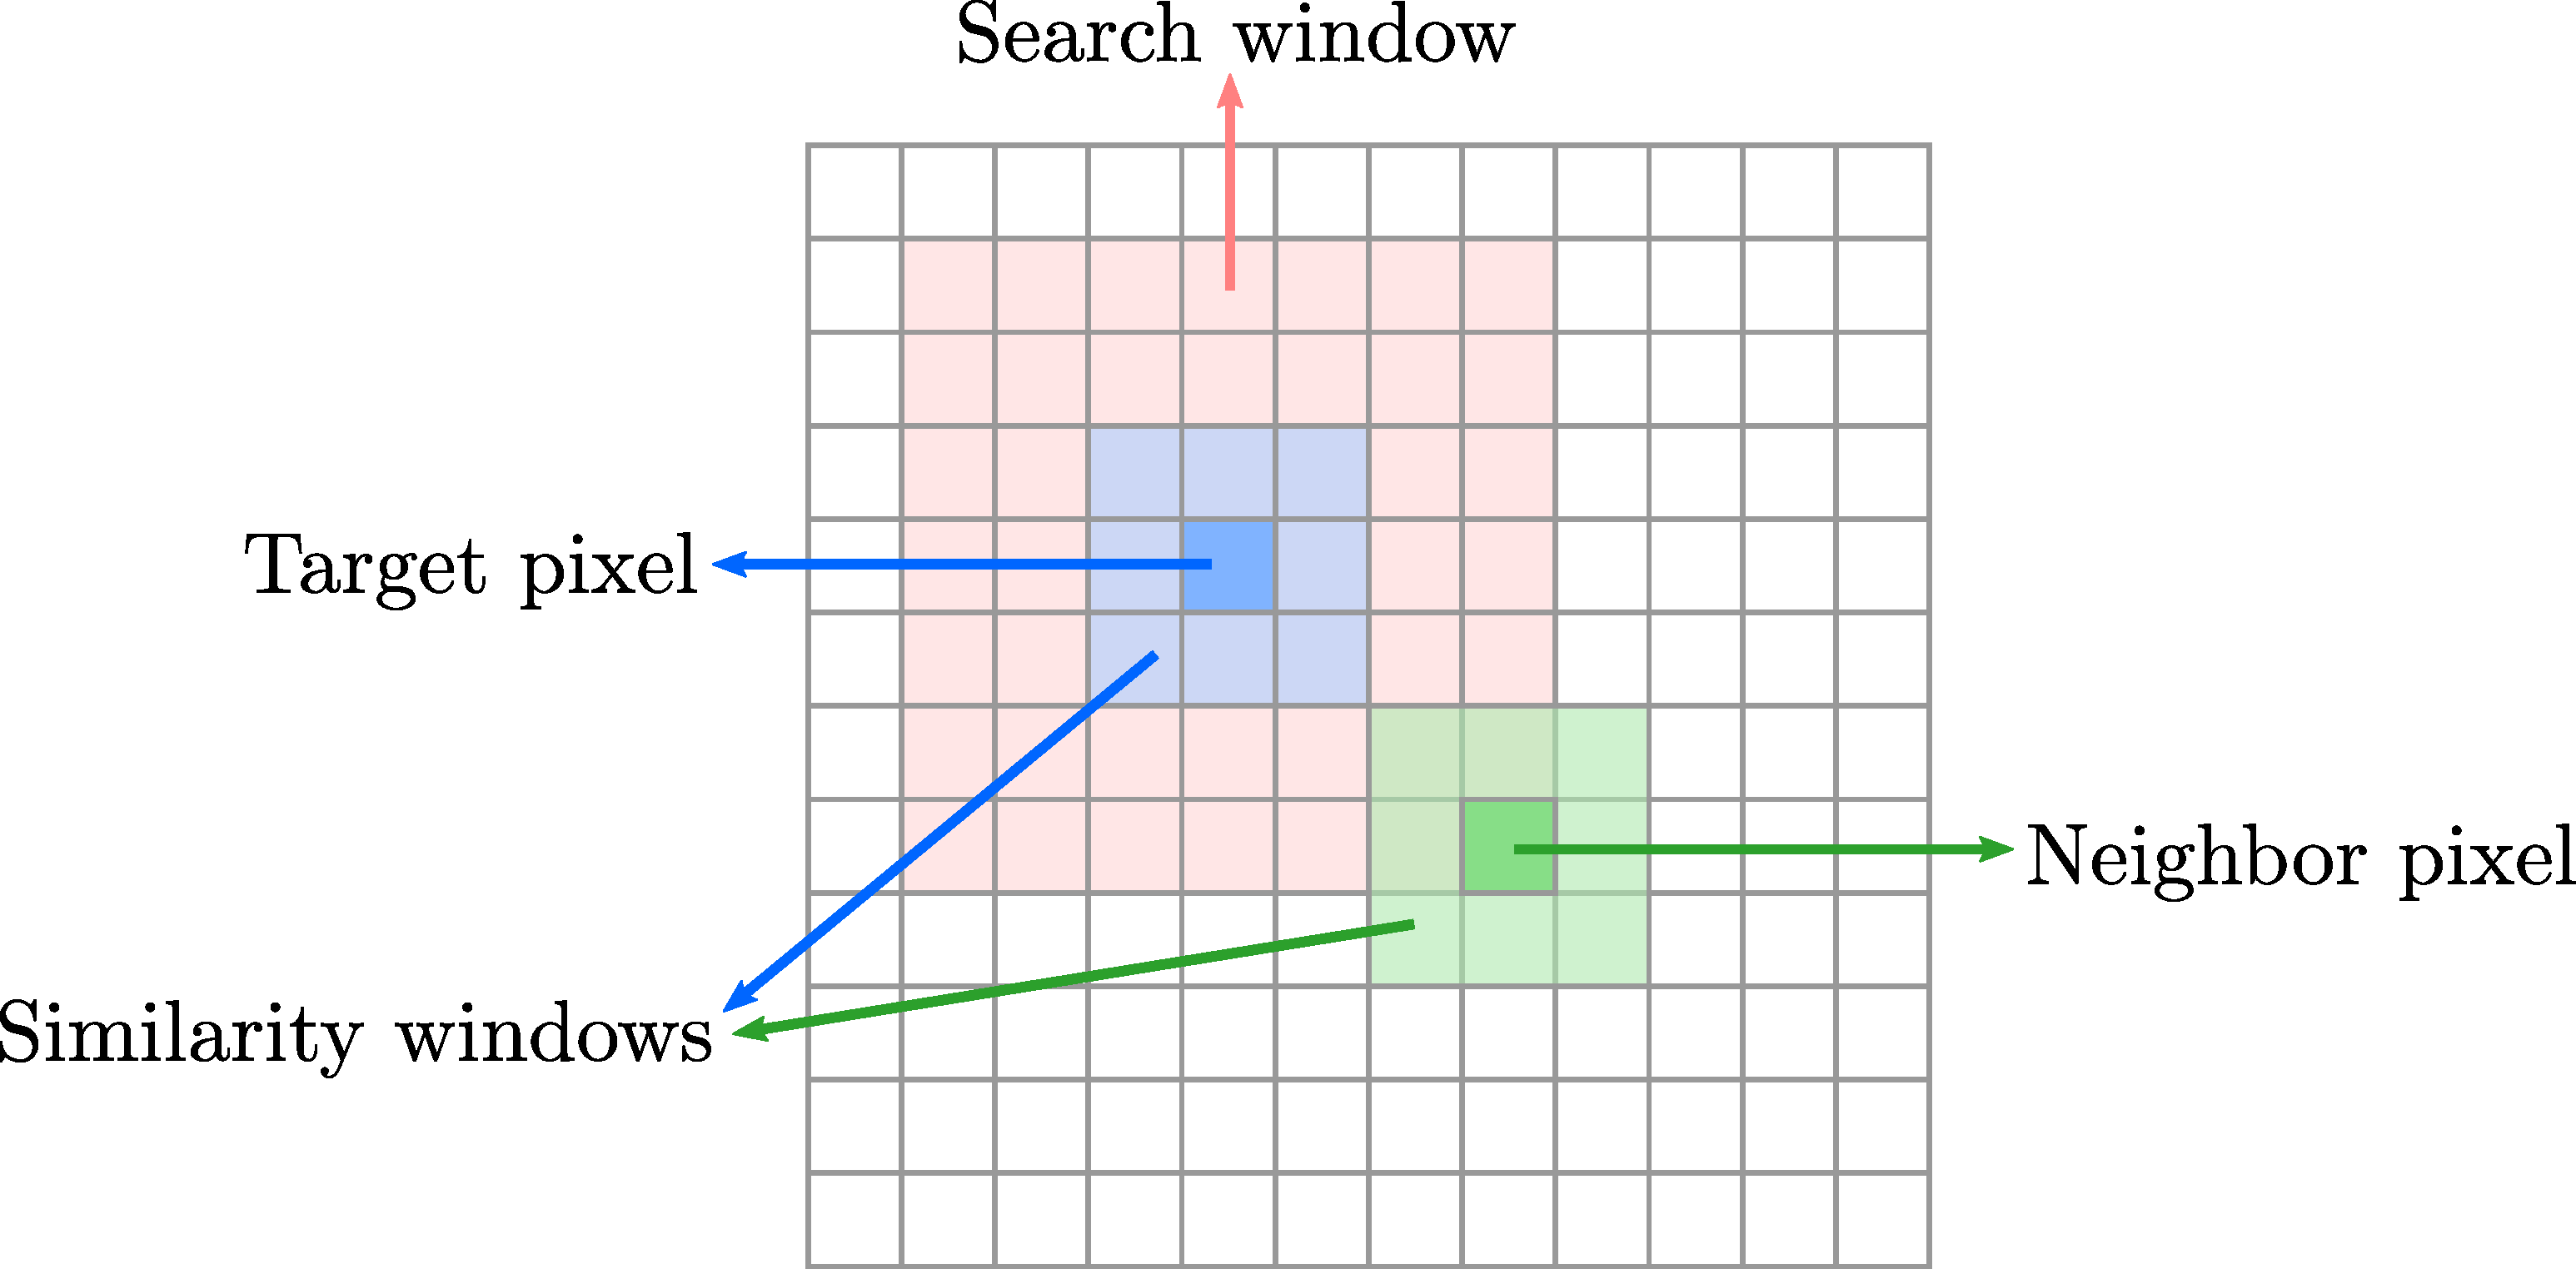
\includegraphics[width=.8\textwidth]{Figures/SHARP/CTNodeScheme.pdf}
	\caption[Illustration of the operation of non-local means.]{Illustration of the operation of non-local means using search window of size 7$\times$7 and similarity windows of size 3$\times$3.}
	\label{fig:CTNodeScheme}
\end{figure}

The purpose of CTNode in the context of this work is to complement SHARP to increase dynamic range of aberration-corrected images. Actually, reduction of complex noise could benefit subsequent operation of SHARP improving the procedure of optimizing image quality in CAO steps in regions with low SNR. Furthermore, there is a wide variety of applications yet to explore where CTNode could also be beneficial, in particular in phase-dependent or complex signal-based techniques like angiography~\cite{Makita2016_Noiseimmune}, flowmetry~\cite{Uribe-Patarroyo2014_Quantitative} and elastography~\cite{Wang2007_Phasesensitive} in which sensitivity is greatly influenced by noise level thus pre-processing the complex signal with CTNode could boots subsequent performance of these techniques, with no need of acquiring multiple repetitions frames as demanded in traditional averaging.

\subsection{Evaluation of CTNode in simulated OCT signal}

To evaluate CTNode, it is desirable to have a noise-free reference but it is in principle impossible to achieve experimentally, therefore, the noise-free simulated OCT tomogram used previously was employed for this purpose. Figure~\ref{fig:CTNode_Sim_int} shows a selected B-scan from the original tomogram in Fig.~\ref{fig:CTNode_Sim_int}(a), showing the cross-section of the bright-intensity cylindrical objects, immersed in the low-intensity nearly homogeneous medium that constitute the tomogram. Synthetic zero-mean Gaussian noise was added to the real and imaginary parts of the noiseless simulated tomogram with a constant variance $\sigma_N^2$ over the entire tomogram, as illustrated with the noisy B-scan of Fig.~\ref{fig:CTNode_Sim_int}(b). There is a signal decay over depth in the original tomogram emulating light absorption, although it may not be obvious in Fig.~\ref{fig:CTNode_Sim_int}(a). This signal decay causes a variation of SNR despite $\sigma_N$ being constant, as can be appreciated in the logarithmic SNR map shown in Fig.~\ref{fig:CTNode_Sim_int}(c), where a threshold was used to display only values greater than $-3$~dB, corresponding to 0.5 in linear scale, which means that the signal level is half the noise variance, hence signal is masked by noise. A limit for the SNR of the minimum detectable signal is 0~dB (1 in linear scale) meaning that the signal level is equal to noise variance.

\begin{figure}[htb!]
	\centering
	\includegraphics[width=\textwidth]{Figures/SHARP/CTNode_Sim_int.pdf}
	\caption[Evaluating performance of CTNode in a simulated OCT tomogram.]{Evaluating performance of CTNode in a simulated OCT tomogram. Intensity B-scan planes: (a) Original noise-free (b) noisy with zero-mean Gaussian noise, (d) after CTNode, after (e) coherent and (f) incoherent averaging. (c) Logarithmic SNR for B-scan in (b) threshold to show only values $>-3$~dB.}
	\label{fig:CTNode_Sim_int}
\end{figure}

Then, CTNode was applied to the noisy tomogram. It was found that the use of large search and similarity windows yields strong noise reduction but at the cost of degrading resolution because the filtering kernel is large and prone to smear information. Conversely, resolution is better preserved using small windows but filtering efficiency is reduced. Furthermore, a large value of $h$ is desired for an efficient noise reduction but it causes a strong filtering of high SNR pixels which are expected to be slightly filtered since effect of noise is not significant. These observations are expected from the general operation of non-local means algorithm and in particular from the operation of TNode for speckle suppression~\cite{Cuartas-Velez2018_Volumetric}. Parameters were iteratively tuned by visual inspection of results seeking for an optimal trade-off between the thee competing aspects: efficient noise reduction, resolution preservation and avoidance of corruption of pixels with high SNR, resulting in a search window of 15$\times$15$\times$15, a similarity window of 3$\times$3$\times$3 and a filtering parameter $h=0.10$. Processing time was about 8~seconds per B-scan of size 160$\times$256~px$^2$, in a workstation computer running on an Intel core i7-8700 processor @~3.2GHz, using a GPU-based implementation in MATLAB 2019a running on a 6~GB GPU NVIDIA P4000.

For comparison, images using coherent and incoherent frames averaging were also computed. The set of repetition frames was created by replicating the noiseless B-scan, then adding synthetic noise to each repetition with the same variance and finally computing the arithmetic mean of the complex signal for coherent averaging and of the intensity signal for incoherence averaging. It is known that coherent averaging of $N$ frames produces a reduction of noise variance by a factor of $1/N$ whereas incoherent averaging only of $1/\sqrt{N}$, however, coherent averaging also reduces signal level resulting in a less SNR improvement than expected, although it is still higher than improvement achieved by incoherent averaging~\cite{Baumann2019_Signal}. For this test, $N$ was set to 12, a value at which coherent averaging performed similar to CTNode. 

Fig.~\ref{fig:CTNode_Sim_int}(d)-(e) shows the noisy B-scan after CTNode, coherent and incoherent averaging, respectively. There is not any signal degradation after CTNode suggesting that its application to the tomogram did not produce any detrimental effect in signal quality, and indeed there is a clear overall reduction of noise level as supposed, compared to noisy B-scan. For the following analysis, two regimes can be identified, one where SNR is below 0~dB and other where SNR is above 0~dB. For $\text{SNR}>0$, CTNode and coherent averaging recovered the underlying signal at an acceptable level, allowing to visually distinguish the speckle pattern from the noise, and in particular the upper dark band can be distinguished from the object information. For incoherent averaging, the speckle pattern is also visually perceptible but the contrast is greatly reduced because in this approach the noise floor level is not reduced, only the noise variance, contrary to coherent average approach where both the noise mean and variance are reduced~\cite{Baumann2019_Signal}. In all cases, the bight intensity structures appear unchanged, as is expected given that noise reduction is less significant when SNR is high. For this reason, noise reduction in intended to improve contrast in regions with SNR approaching to zero, whereas in regions with high SNR it is unlikely necessary because contribution of noise is unimportant. 

For $\text{SNR}<0$~dB, it can be observed that despite the noise reduction, underlying signal information is lost in all filtering approaches, since in this regime the mean intensity signal is below the noise variance and therefore underlying true signal cannot be distinguishable from noise. In fact, it is possible to increase negative SNRs values using coherent average and for this case it was achieved at $N=100$ which is a relatively large and possibly unpractical amount.

The relevance of complex noise reduction is not only evident in intensity images in terms of contrast improvement but also in phase information that is very susceptible to noise. Figure~\ref{fig:CTNode_Sim_Phase} shows phase images of the B-scan plane used for Fig.~\ref{fig:CTNode_Sim_int}, of the original and noisy tomogram in Figs.~\ref{fig:CTNode_Sim_Phase}(a) and (b). Speckle pattern is directly visualized in noiseless phase B-scan, whereas noisy phase shows regions dominated by noise, and even in the high SNR regions noise is perceptible, making difficult the visualization of speckle pattern. Phase B-scans after CTNode and coherent averaging are shown in Fig.~\ref{fig:CTNode_Sim_Phase}(c) and (d), respectively, and both exhibit a reduction of noise in high and low SNR regimes, recovering the speckle pattern lost in low SNR regions and improving visualization of high SNR regions. 

% \begin{figure}[htb!]
% 	\centering
% 	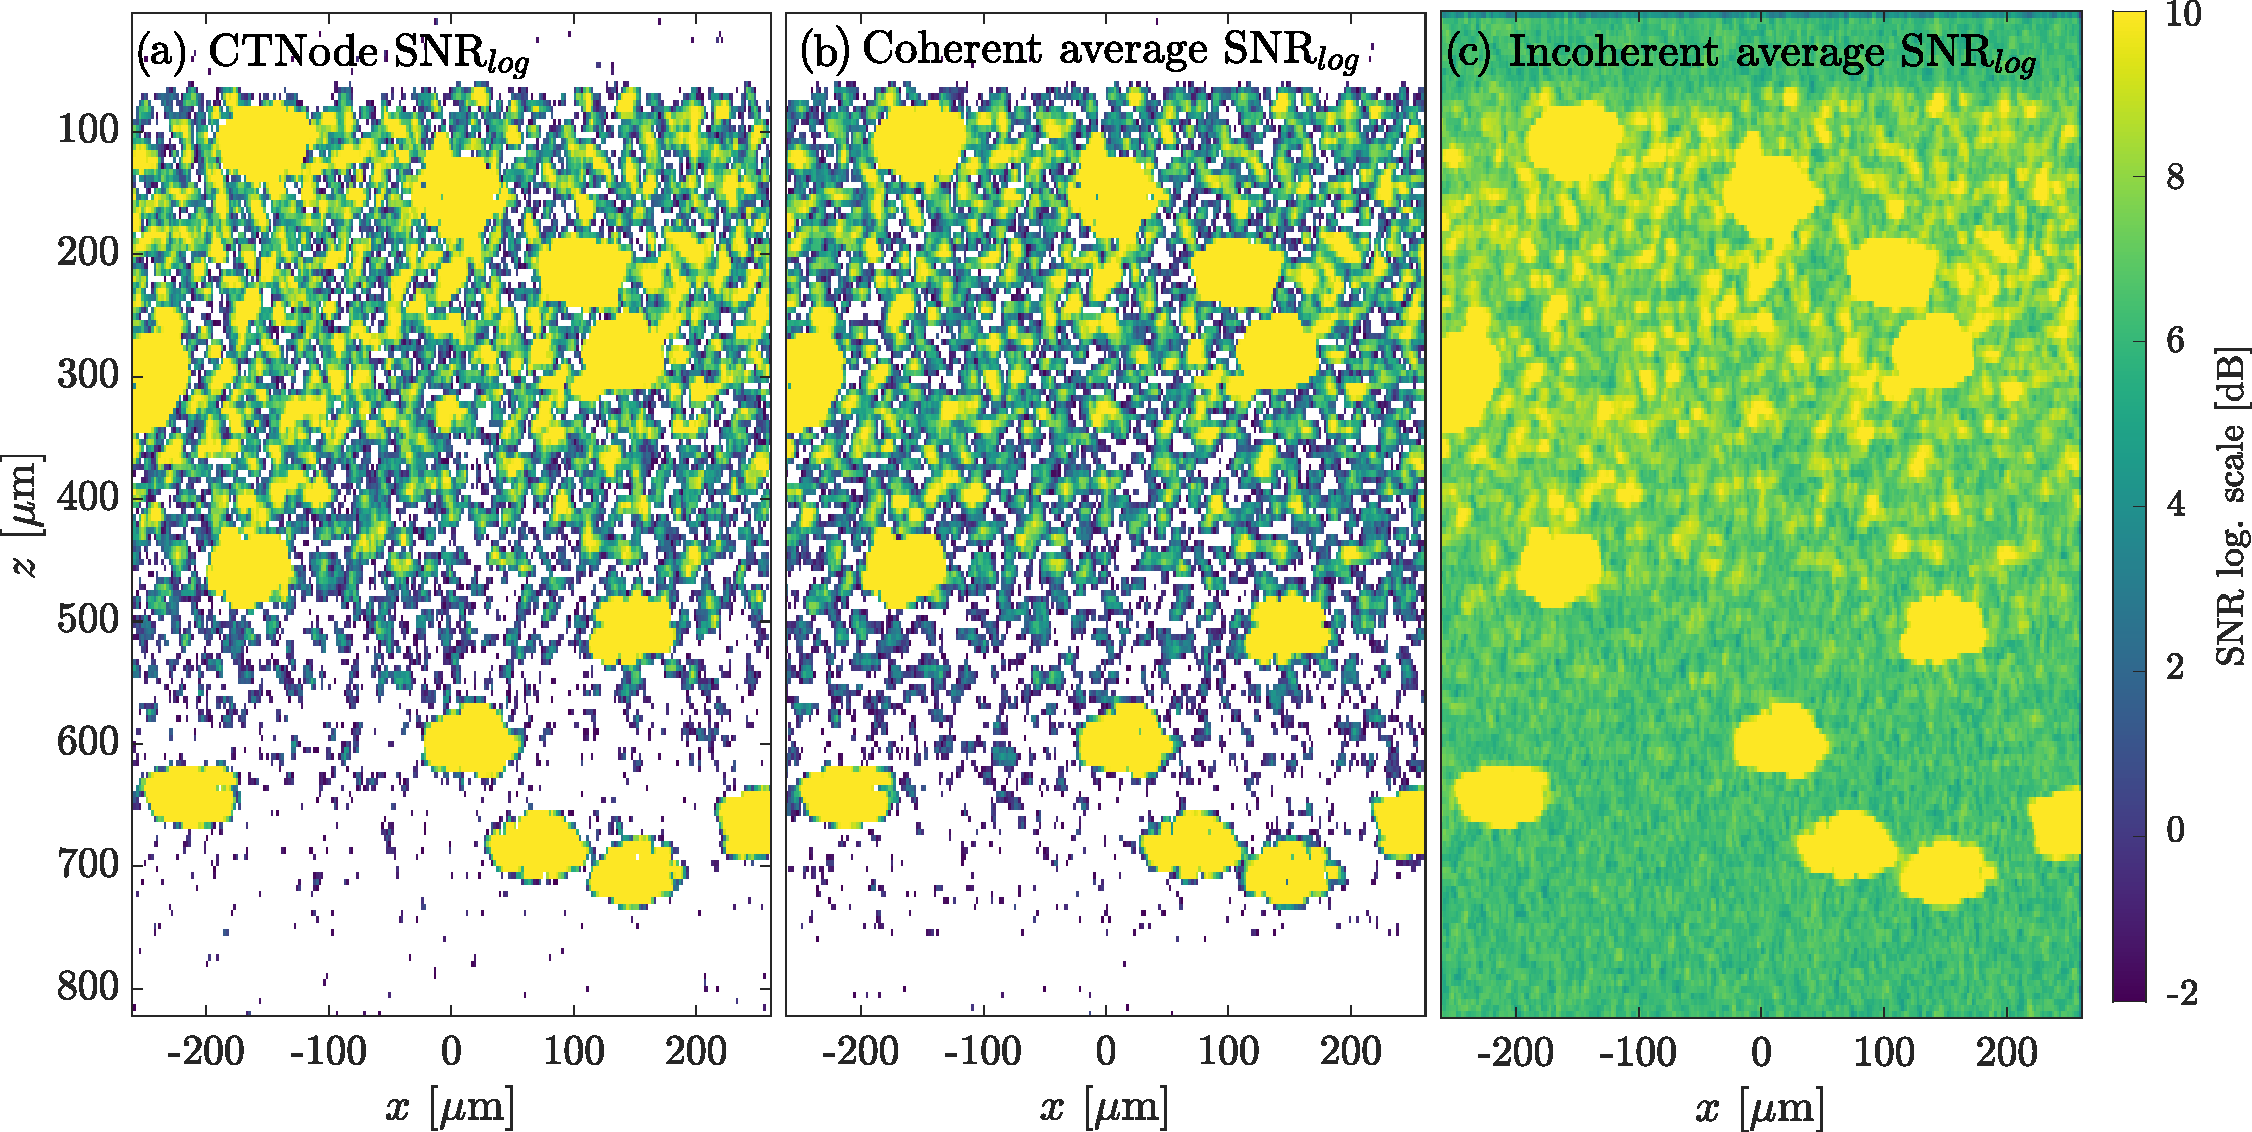
\includegraphics[width=\textwidth]{Figures/SHARP/CTNode_Sim_SNR.pdf}
% 	\caption[.]{.}
% 	\label{fig:CTNode_Sim_SNR}
% \end{figure}

\begin{figure}[htb!]
	\centering
	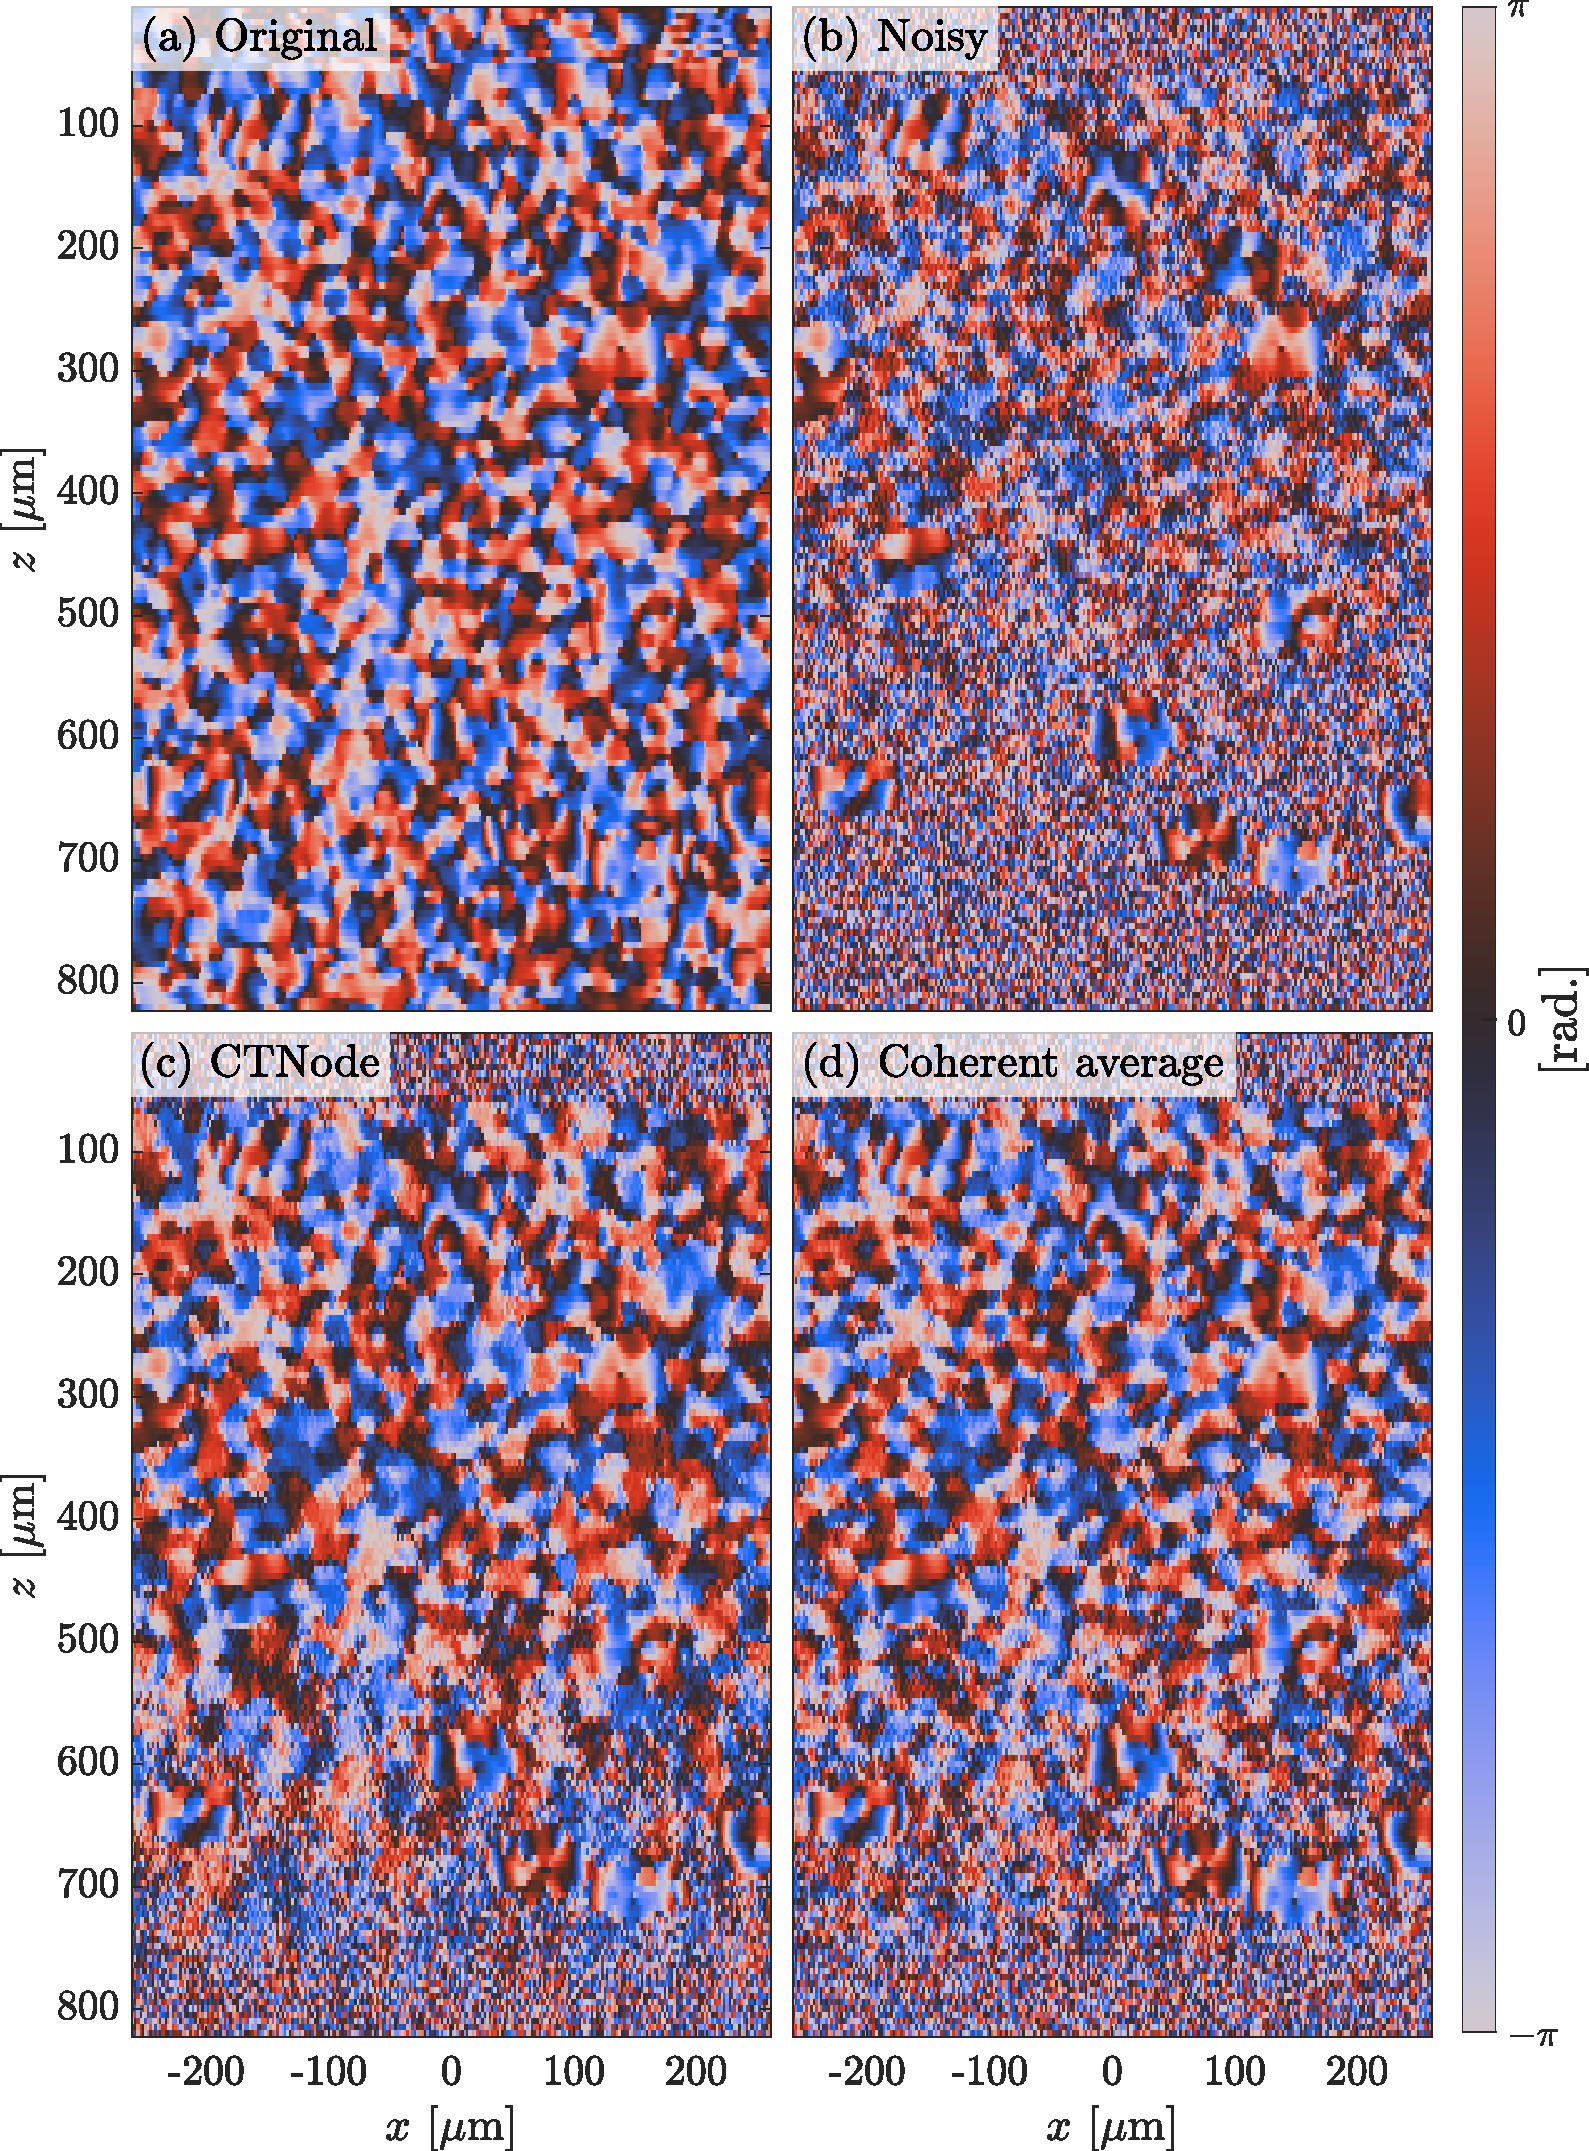
\includegraphics[width=.7\textwidth]{Figures/SHARP/CTNode_Sim_Phase.pdf}
	\caption[Evaluating reduction of Gaussian noise in phase information with CTNode in a simulated OCT tomogram.]{Evaluating reduction of Gaussian noise in phase information with CTNode in a simulated OCT tomogram. B-scan phase images: (a) Original noise-free, (b) noisy with zero-mean Gaussian noise and then filtered (c) with CTNode and (d) with coherent wavering.}
	\label{fig:CTNode_Sim_Phase}
\end{figure}

Although with current implementation of CTNode it appears to be unfeasible to filter pixels with negative SNRs to recover the underlying signal properly, it is clear that CTNode outperforms coherent averaging in the sense that it required a single repetition to obtain a similar result of averaging $12$ repetitions, given that CTNode (and non-local means in general) efficiently exploits the available information. It is expectable that extension of CTNode to operate with multiple frame repetitions, like it is possible with TNode currently, could boost its operation even more compared to arithmetic frame averaging. Anyhow, the possibility to efficiently reduce complex noise with a single acquisition is attractive for phase-dependent techniques where multiple repetition of frames is not practical given its specific acquisition scenarios~\cite{Uribe-Patarroyo2020_Noise}.
